\documentclass[11pt,a4paper]{report}
\usepackage[utf8]{inputenc}
\usepackage[T1]{fontenc}
\usepackage[spanish,es-noshorthands,es-tabla]{babel}
\usepackage{lmodern}
\usepackage{microtype}
\usepackage[a4paper,margin=2.2cm,headheight=14pt]{geometry}
\usepackage{graphicx}
\usepackage{float}
\usepackage{rotating}
\usepackage{xcolor}
\usepackage{booktabs}
\usepackage{amssymb}
\usepackage{tabularx}
\usepackage{longtable}
\usepackage{array}
\usepackage{titlesec}
\usepackage{fancyhdr}
\usepackage{enumitem}
\usepackage{listings}
\usepackage{caption}
\usepackage[most]{tcolorbox}
\usepackage[hidelinks,bookmarksnumbered]{hyperref}

\definecolor{marca}{HTML}{8B1E3F}
\definecolor{tinta}{HTML}{1F2933}
\definecolor{suave}{HTML}{F7F2F4}
\definecolor{verbget}{HTML}{1F6F43}
\definecolor{verbpost}{HTML}{1D4E89}
\definecolor{verbpatch}{HTML}{8A5A00}
\definecolor{verbdelete}{HTML}{9B1C1C}

\titleformat{\chapter}[display]{\normalfont\bfseries\color{marca}}{\large\MakeUppercase{\chaptertitlename}\ \thechapter}{4pt}{\Huge}
\titlespacing*{\chapter}{0pt}{-10pt}{16pt}
\titleformat{\section}{\normalfont\Large\bfseries\color{tinta}}{\thesection}{0.8em}{}
\titleformat{\subsection}{\normalfont\large\bfseries\color{marca}}{\thesubsection}{0.8em}{}

\pagestyle{fancy}
\fancyhf{}
\fancyhead[L]{\small\color{gray}xChanger --- Modelos de Requisitos y Arquitectura}
\fancyhead[R]{\small\color{gray}v1.0}
\fancyfoot[C]{\small\thepage}

\captionsetup{font=small,labelfont=bf}
\setlength{\parskip}{0.45em}
\setlength{\parindent}{0pt}

\newcommand{\verbo}[2]{\colorbox{#1}{\textcolor{white}{\ttfamily\bfseries\small #2}}}
\newtcolorbox{apiendpoint}[2]{enhanced,breakable,colback=white,colframe=marca!45,colbacktitle=suave,
  coltitle=tinta,fonttitle=\small,title={#1\hfill\textnormal{\footnotesize Acceso: #2}},
  boxrule=0.5pt,arc=1.5pt,left=5pt,right=5pt,top=4pt,bottom=4pt,before skip=7pt,after skip=7pt,fontupper=\small}

% PlantUML en listings (con caracteres españoles y guillemets)
\lstdefinelanguage{plantuml}{
  morekeywords={@startuml,@enduml,actor,participant,database,usecase,rectangle,package,class,enum,component,interface,node,note,end,alt,else,opt,loop,par,group,autonumber,title,left,right,top,bottom,of,as,state,skinparam,hide,include},
  sensitive=true, morecomment=[l]{'}, morestring=[b]"}
\lstset{basicstyle=\ttfamily\scriptsize,keywordstyle=\color{marca}\bfseries,commentstyle=\color{gray},
  stringstyle=\color{verbpost},breaklines=true,columns=fullflexible,frame=single,rulecolor=\color{gray!40},
  backgroundcolor=\color{suave},extendedchars=true,
  literate={á}{{\'a}}1 {é}{{\'e}}1 {í}{{\'i}}1 {ó}{{\'o}}1 {ú}{{\'u}}1 {ñ}{{\~n}}1
           {Á}{{\'A}}1 {É}{{\'E}}1 {Í}{{\'I}}1 {Ó}{{\'O}}1 {Ú}{{\'U}}1 {Ñ}{{\~N}}1 {ü}{{\"u}}1
           {«}{{\guillemotleft}}1 {»}{{\guillemotright}}1 {—}{{---}}1 {–}{{--}}1 {×}{{$\times$}}1
           {¿}{{?`}}1 {¡}{{!`}}1 {§}{{\S}}1 {→}{{$\rightarrow$}}1 {↔}{{$\leftrightarrow$}}1}

\begin{document}

\begin{titlepage}
\centering
\vspace*{3cm}
{\color{marca}\rule{\linewidth}{1pt}}\\[0.6cm]
{\Huge\bfseries xChanger\\[0.3cm]}
{\LARGE Modelos de Requisitos y Arquitectura\\[0.3cm]}
{\large Casos de uso, dominio, acciones, componentes y especificación de la API}\\[0.4cm]
{\color{marca}\rule{\linewidth}{1pt}}\\[2cm]
\begin{tabular}{@{}ll@{}}
\toprule
Proyecto & xChangerMejorado \\
Notación & UML 2.5 (diagramas generados con PlantUML), OCL 2.4 para restricciones \\
Documentos base & Requisitos v1.0; Arquitectura v1.0; Escalado v1.0 \\
Alcance de la API & Core: 80 endpoints de \texttt{/api/v1} \\
Fecha & Noviembre de 2026 \\
Versión & 1.0 \\
\bottomrule
\end{tabular}
\vfill
{\small Este documento complementa la Especificación de Requisitos: no repite los requisitos, los modela. Los identificadores RF-, RA-, RNF-, CA- remiten a Requisitos v1.0; ADR-16+, EP-, RF-TGB- y RF-MFA- al documento de Escalado.}
\end{titlepage}

\tableofcontents

%════════════════════════════════════════════════════════════════════
\chapter{Introducción}

\section{Propósito y alcance}
Este documento reúne los modelos que el equipo necesita para construir y mantener xChanger: qué hace el sistema para cada actor y por cada interfaz, qué información maneja, cómo se comporta como caja negra en los flujos críticos, cómo se descompone en componentes y cómo colaboran estos, y el contrato completo de la API del core.

El sistema modelado es la plataforma xChanger tras el escalado: el \emph{core} (monolito modular Express + Prisma + Socket.io), el frontend Astro, y dos microservicios satélite, el bot de Telegram y el mfa-service. Los modelos de requisitos tratan la plataforma como una unidad; los de arquitectura la abren.

\section{Convenciones de notación}
\begin{itemize}[leftmargin=*,itemsep=1pt]
\item \textbf{Casos de uso.} El rectángulo es el sujeto (el sistema). Los actores primarios están a la izquierda y los secundarios (estereotipo \guillemotleft sistema\guillemotright) a la derecha. Las asociaciones actor–caso de uso no tienen dirección. \guillemotleft include\guillemotright{} apunta del caso base al incluido; \guillemotleft extend\guillemotright{} apunta del caso extensor al base e indica su condición entre llaves.
\item \textbf{Clases.} Modelo conceptual: sin claves foráneas ni detalles de persistencia. Composición (rombo relleno) cuando la parte no existe sin el todo; asociación navegable cuando solo interesa un sentido. Las restricciones que el diagrama no puede expresar se escriben en OCL.
\item \textbf{Secuencia.} Los diagramas de sistema (DSS) muestran \texttt{:xChanger} como una sola línea de vida. Los internos (DSI) usan instancias anónimas de componentes (\texttt{:Nombre}). Los mensajes asíncronos usan punta abierta; los fragmentos \texttt{alt}, \texttt{opt}, \texttt{loop}, \texttt{par} y \texttt{group} siguen UML 2.5.
\item \textbf{Componentes.} Interfaz proporcionada: piruleta unida al componente. Interfaz requerida: dependencia \guillemotleft use\guillemotright{} hacia la interfaz. \guillemotleft delegate\guillemotright{} conecta un subcomponente con la interfaz que expone su contenedor.
\end{itemize}
Las fuentes PlantUML de todos los diagramas están en el Apéndice~\ref{ap:fuentes}.

%════════════════════════════════════════════════════════════════════
\chapter{Modelos de requisitos}

\section{Modelo de casos de uso}

\subsection{Actores}
\begin{center}\small
\begin{tabularx}{\linewidth}{@{}p{3.6cm}p{2.6cm}p{2.3cm}X@{}}
\toprule
Actor & Tipo & Interfaz & Descripción \\
\midrule
Visitante & Primario & Web & Persona sin sesión: se registra, consulta el catálogo e inicia sesión.\\
Usuario registrado & Primario & Web & Cualquier persona con cuenta, antes de autenticarse.\\
Estudiante & Primario & Web, Telegram & Usuario base: expediente, ofertas, chat, tickets, notificaciones y seguridad de su cuenta.\\
Embajador & Primario & Web & Especialización de Estudiante con ámbito (carrera, curso): administra estructura, tickets, bloqueos y auditoría.\\
Propietario & Primario & Web & Especialización de Embajador con ámbito total: carreras, embajadores y ámbitos.\\
Usuario de Telegram no vinculado & Primario & Telegram & Persona que habla con el bot sin identidad vinculada.\\
telegram-bot & Primario (sistema) & API de servicios & Microservicio adaptador de canal; actúa con credencial de servicio y, en nombre del usuario, con token de canal.\\
mfa-service & Secundario (sistema) & API de servicios & Custodio de los factores XOTP; el core lo invoca para enrolar y verificar, y él consulta el JWKS del core.\\
Servidor SMTP & Secundario (sistema) & — & Entrega los OTP y las notificaciones por correo.\\
App autenticadora & Externo (sin interacción) & — & Genera los códigos a partir del QR; no se comunica con el sistema.\\
Orquestador & Primario (sistema) & API de servicios & Docker o monitorización: consulta la salud.\\
\bottomrule
\end{tabularx}
\end{center}
La generalización Estudiante $\leftarrow$ Embajador $\leftarrow$ Propietario hace que cada actor herede los casos de uso de su ancestro, de acuerdo con la matriz de roles (Tabla 6 de Requisitos). El rol Bloqueado no es un actor: es un estado del Estudiante que le impide iniciar cualquier caso de uso.

\subsection{Interfaz web: visitante y acceso}
\begin{figure}[H]\centering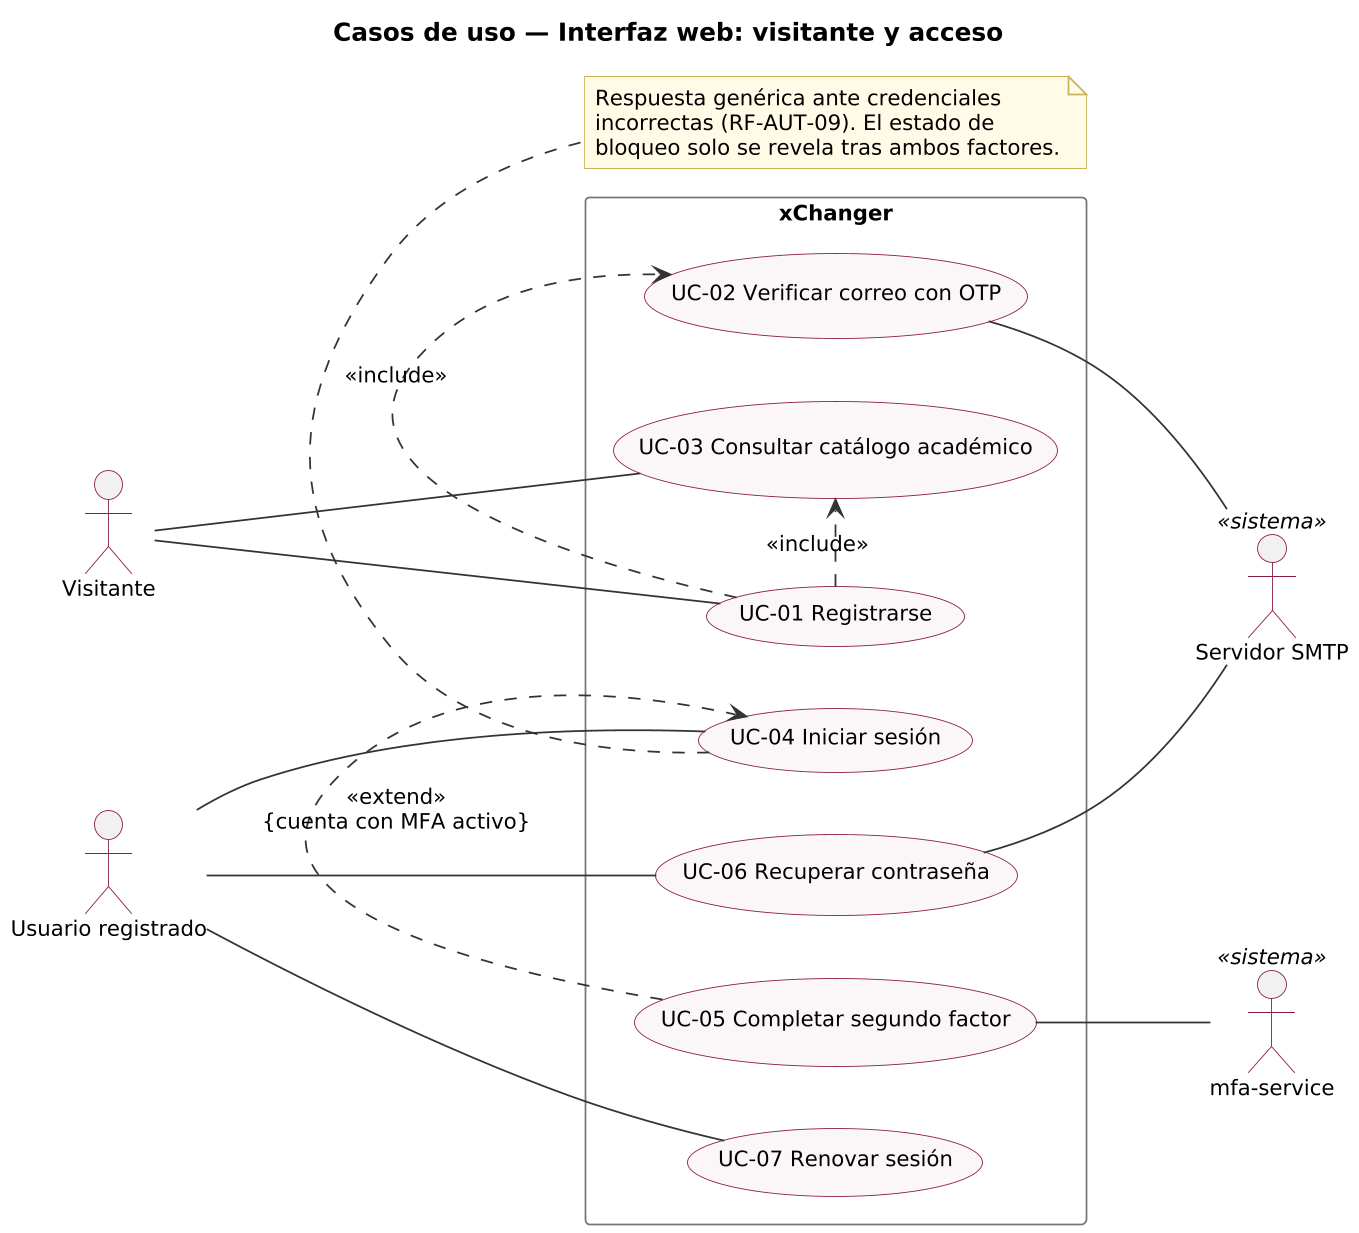
\includegraphics[width=0.75\linewidth,height=0.80\textheight,keepaspectratio]{img/uc01-web-visitante.png}\caption{Casos de uso de acceso desde la web.}\label{fig:uc01-web-visitante}\end{figure}

\subsection{Interfaz web: estudiante}
\begin{figure}[H]\centering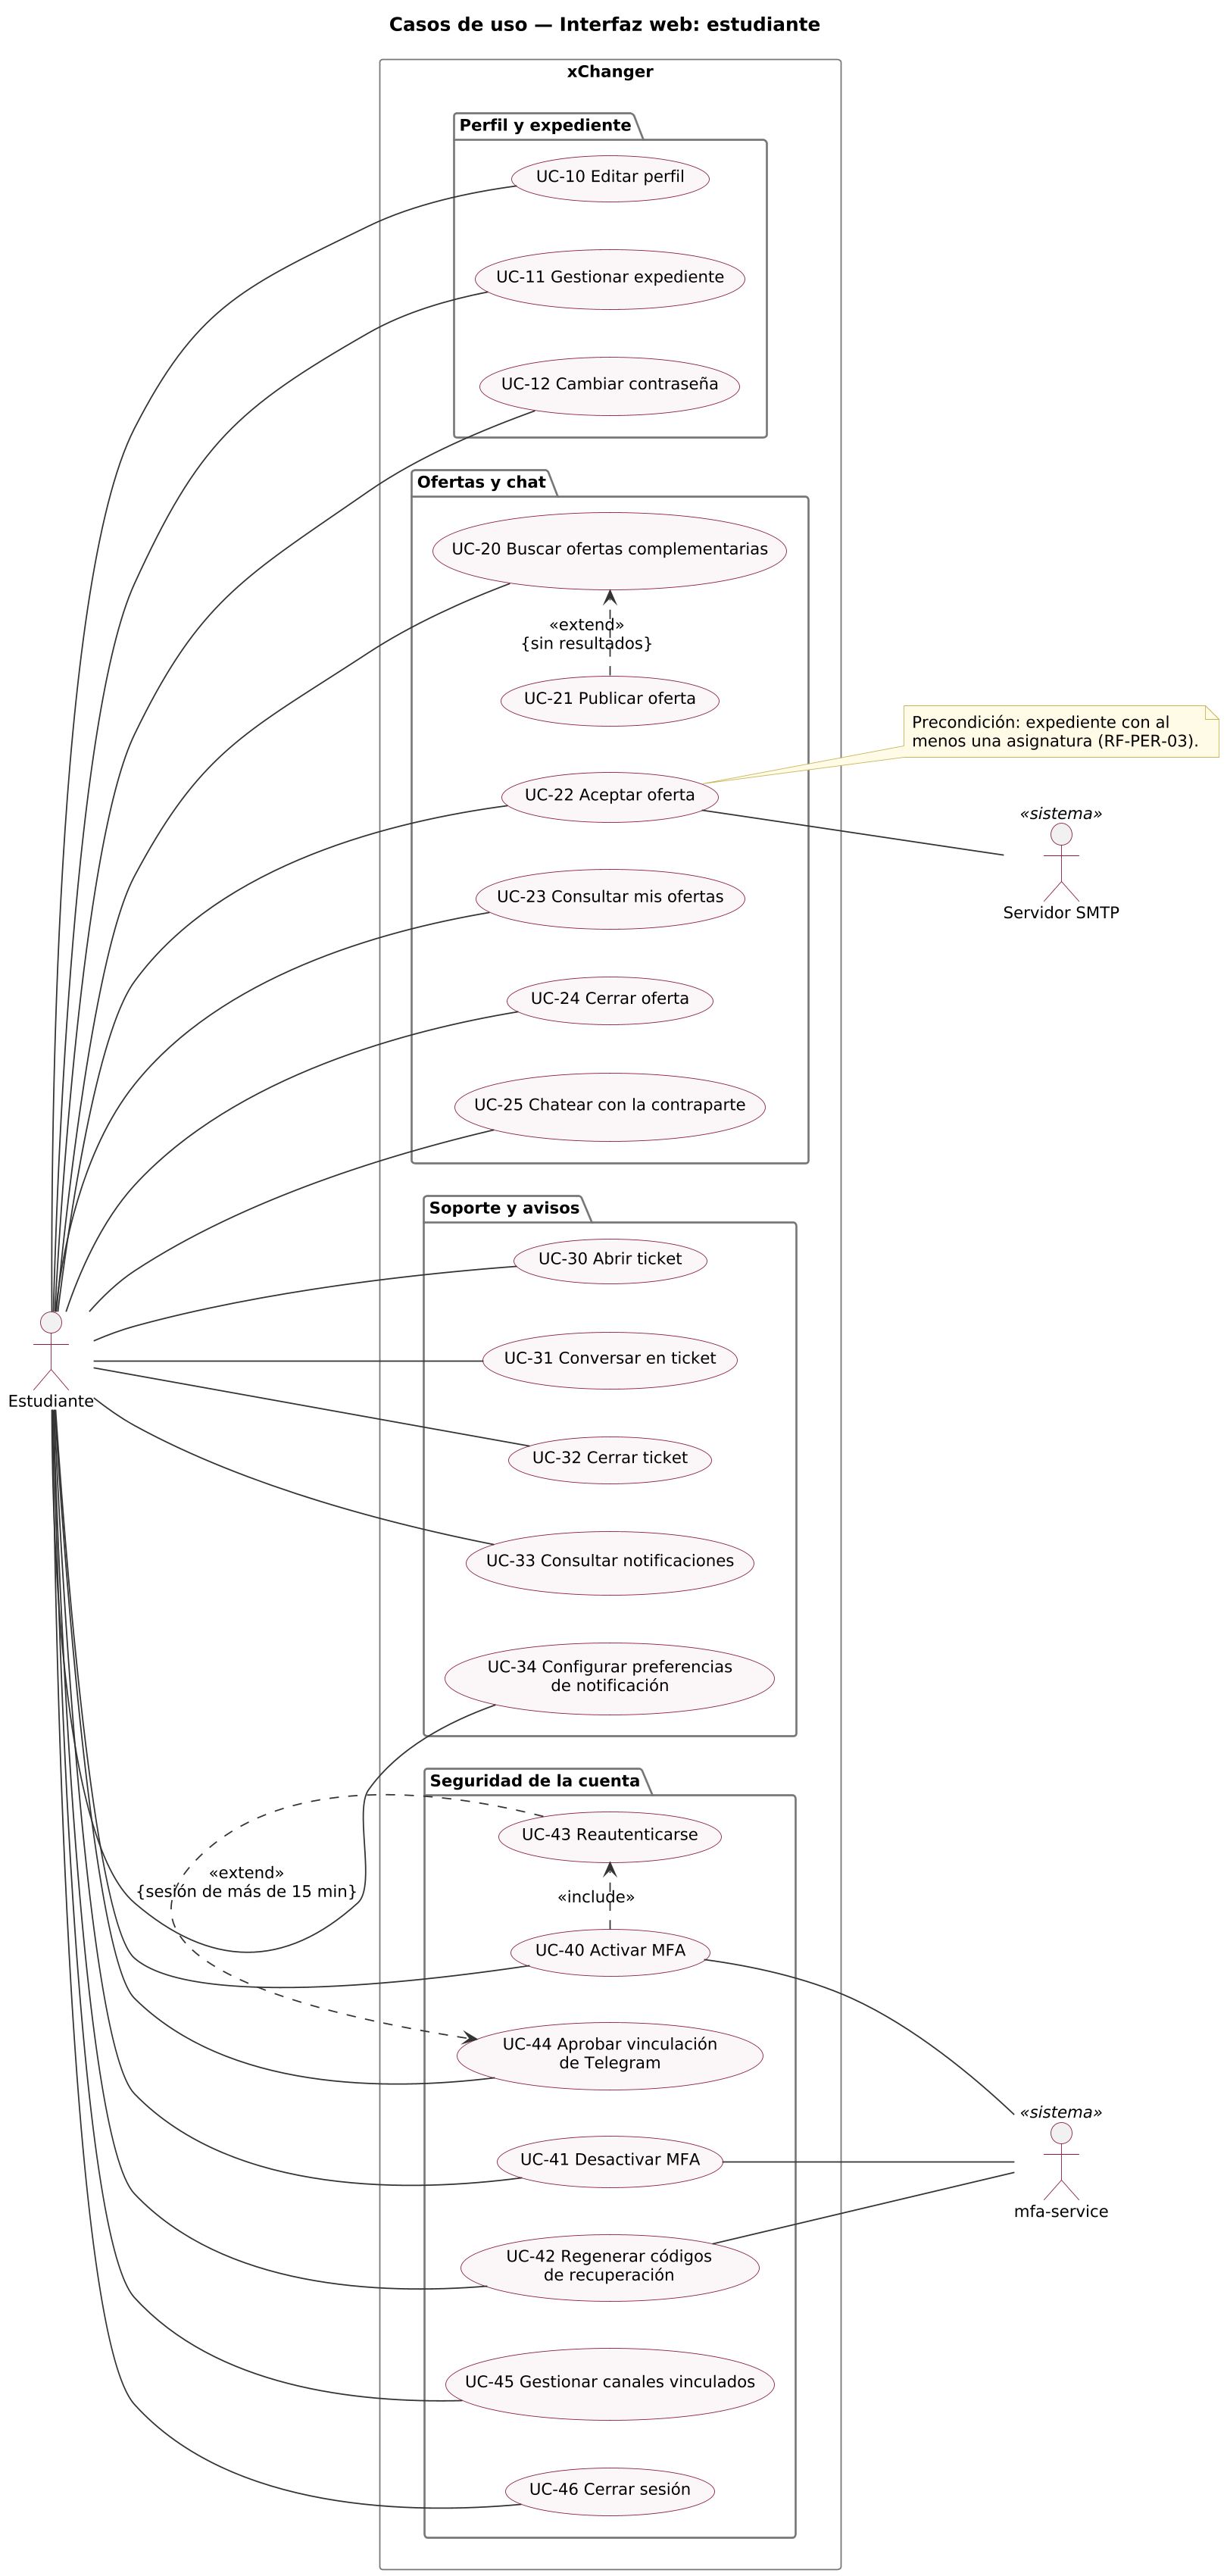
\includegraphics[width=0.68\linewidth,height=0.80\textheight,keepaspectratio]{img/uc02-web-estudiante.png}\caption{Casos de uso del estudiante en la web.}\label{fig:uc02-web-estudiante}\end{figure}

\subsection{Interfaz web: administración}
\begin{figure}[H]\centering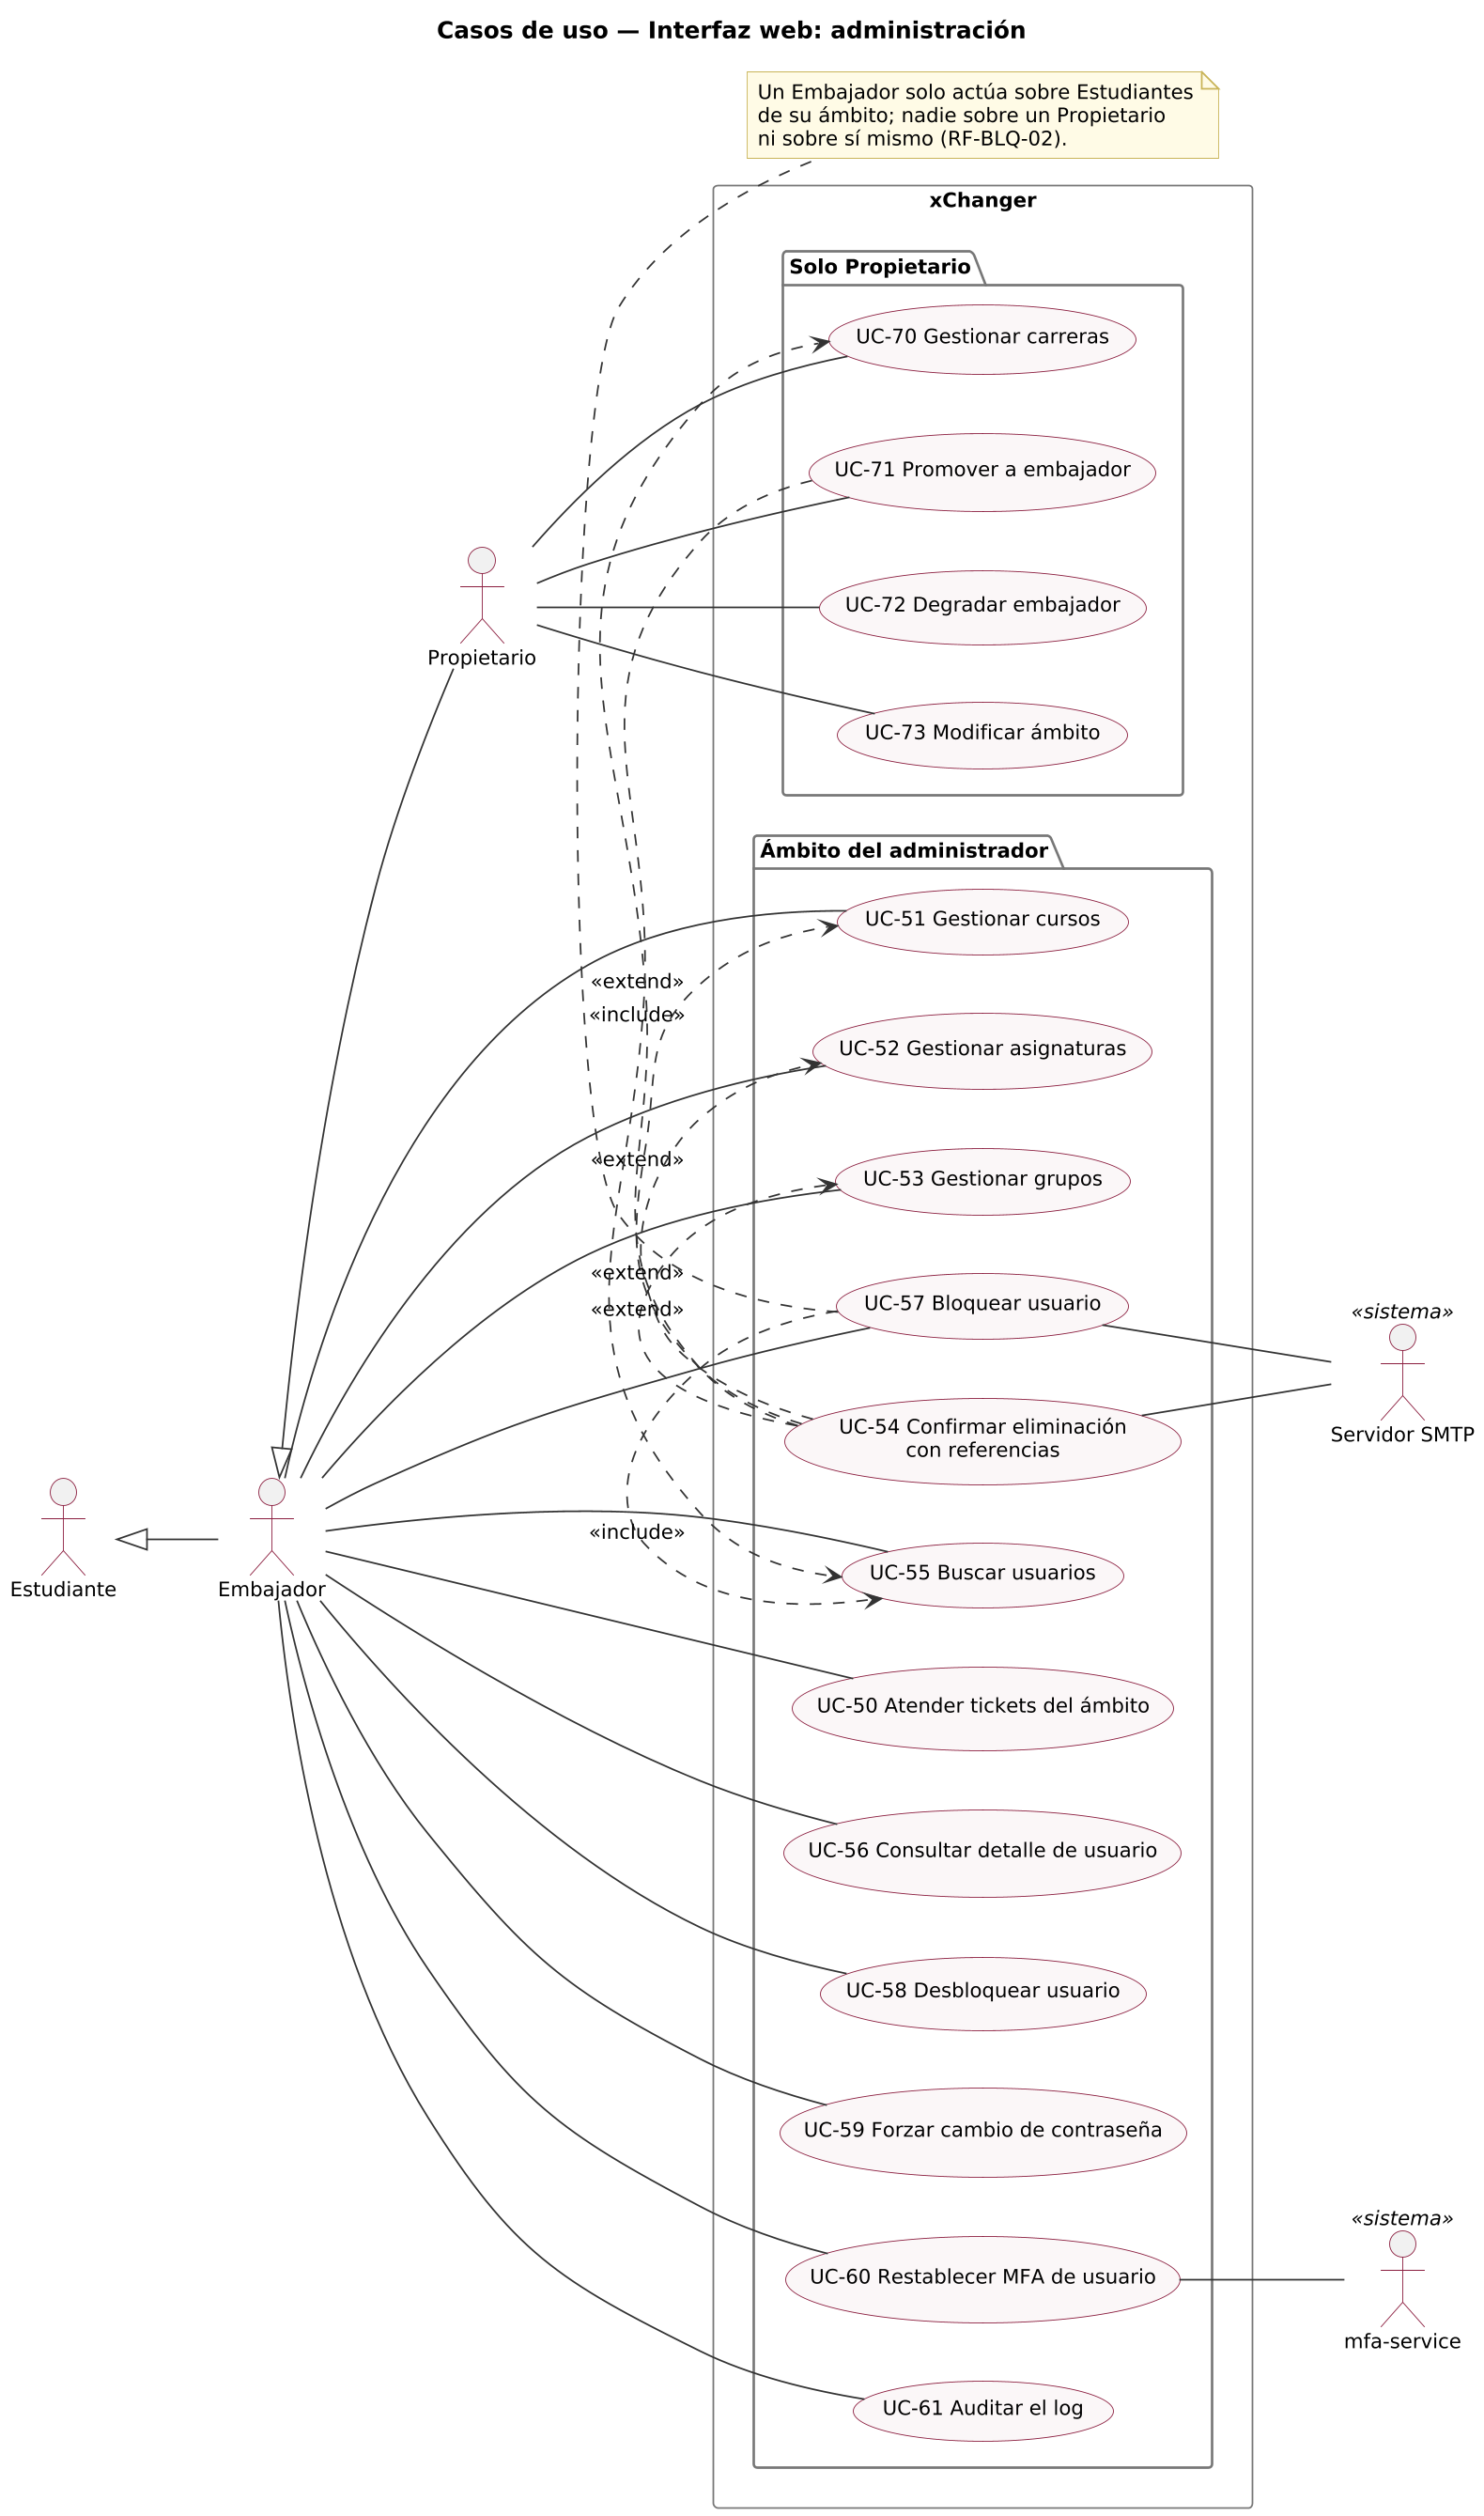
\includegraphics[width=0.70\linewidth,height=0.80\textheight,keepaspectratio]{img/uc03-web-administracion.png}\caption{Casos de uso de administración. Un Propietario hereda todos los del Embajador.}\label{fig:uc03-web-administracion}\end{figure}

\subsection{Interfaz Telegram}
\begin{figure}[H]\centering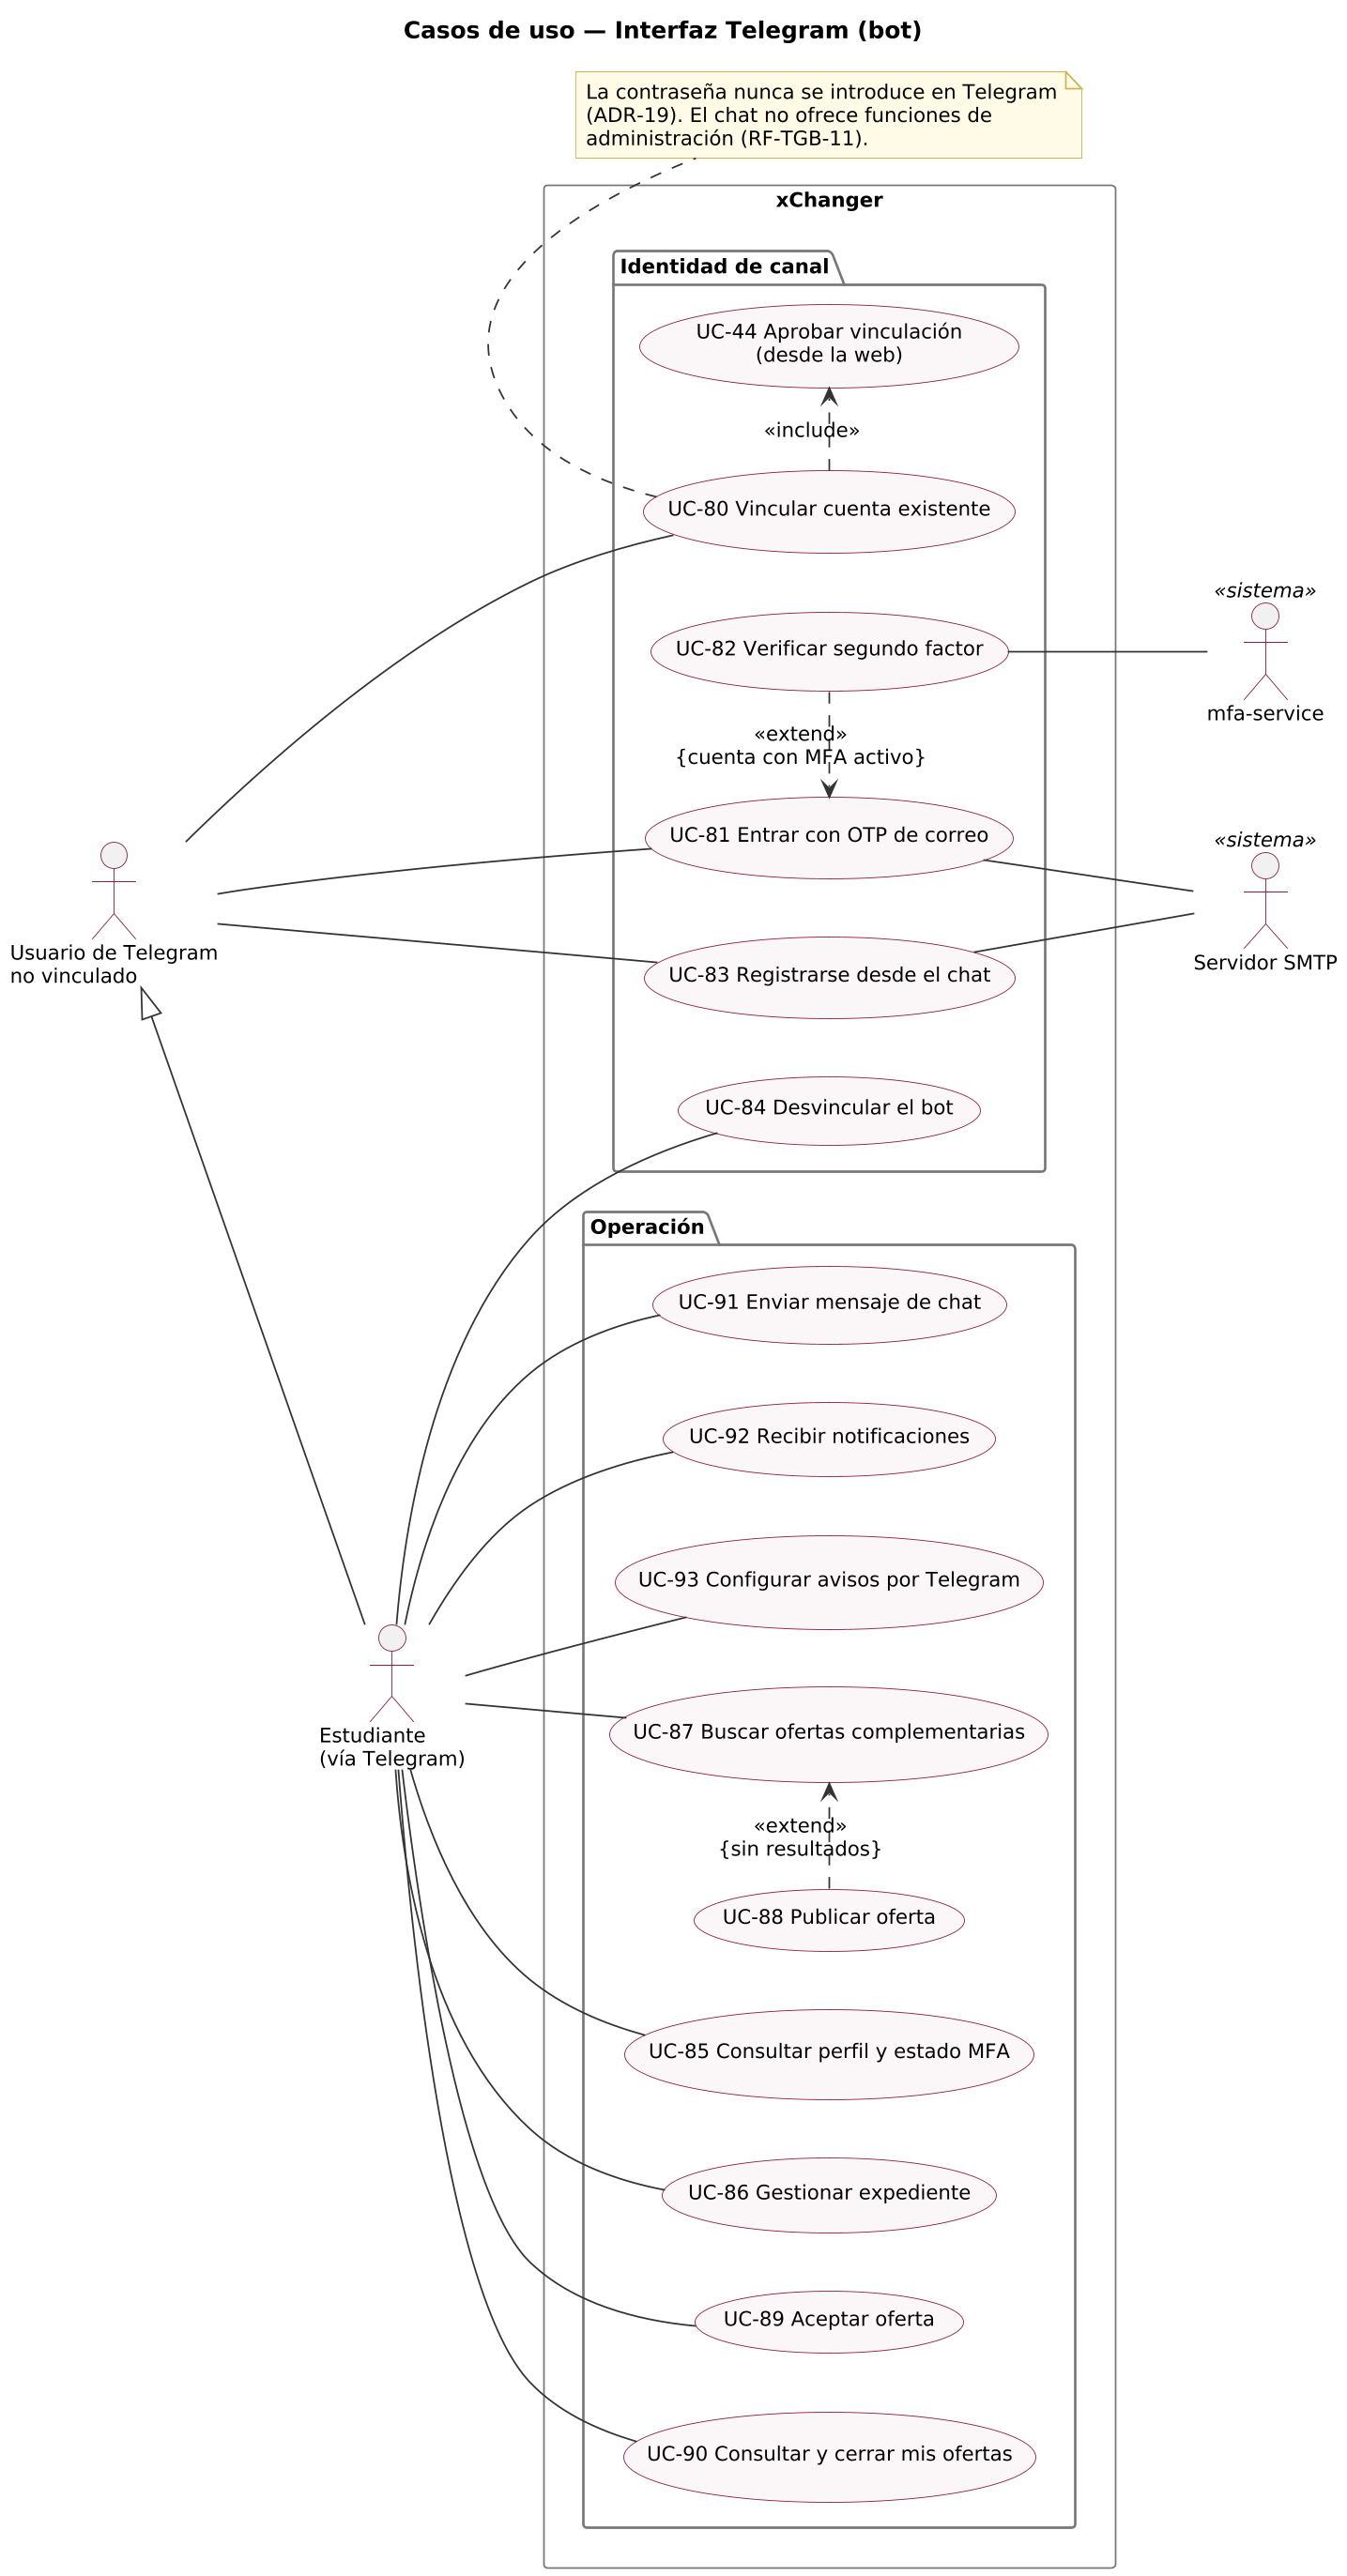
\includegraphics[width=0.62\linewidth,height=0.80\textheight,keepaspectratio]{img/uc04-telegram.png}\caption{Casos de uso por el bot de Telegram. UC-44 se realiza en la web, por eso aparece incluido.}\label{fig:uc04-telegram}\end{figure}

\subsection{Interfaz de servicios (máquina a máquina)}
\begin{figure}[H]\centering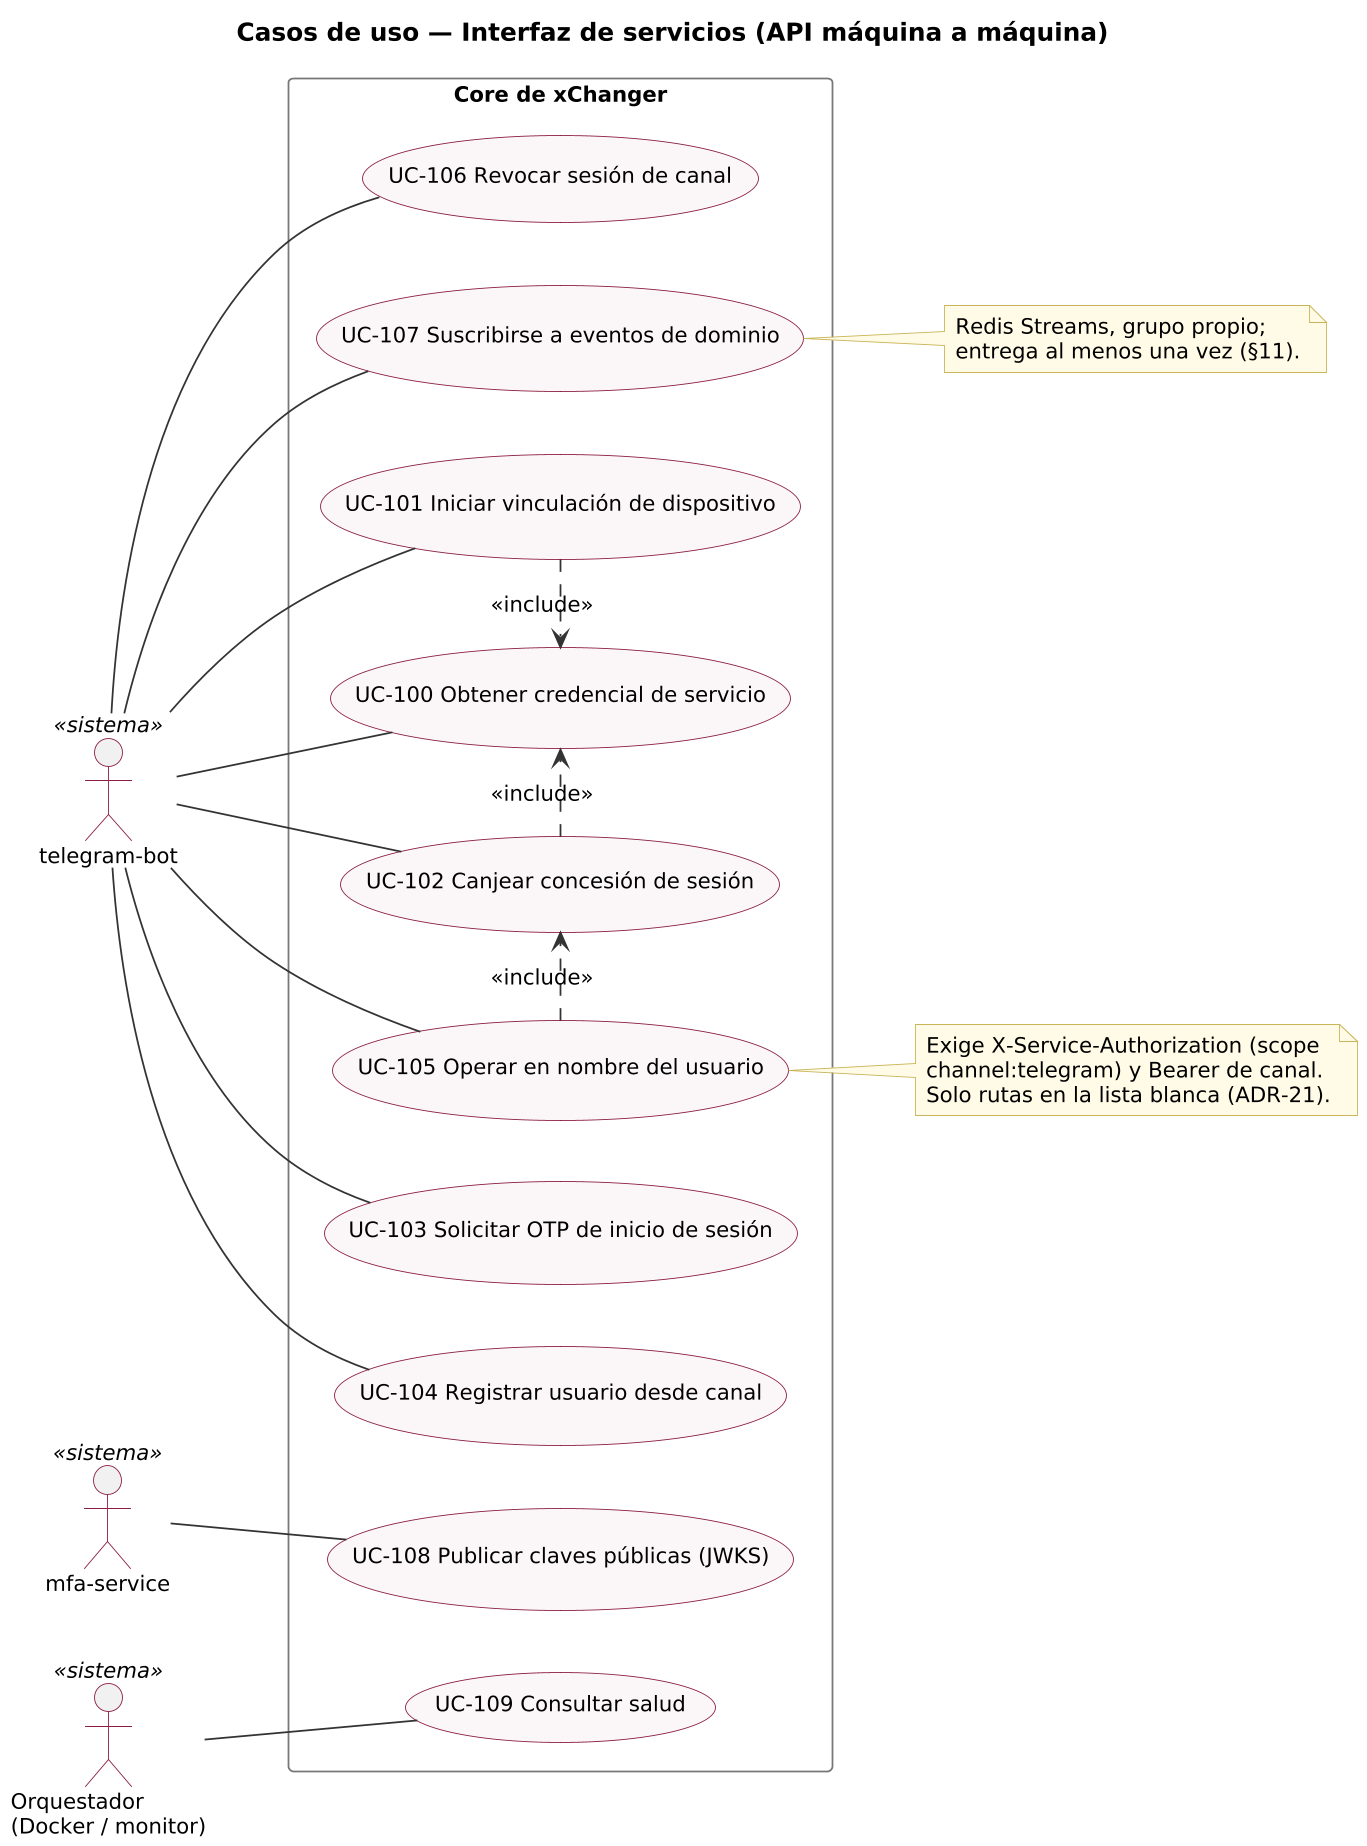
\includegraphics[width=0.75\linewidth,height=0.80\textheight,keepaspectratio]{img/uc05-api-servicios.png}\caption{Casos de uso de la API de servicios. El sujeto es el core.}\label{fig:uc05-api-servicios}\end{figure}

\subsection{Catálogo de casos de uso}
\begin{center}\small
\begin{longtable}{@{}lp{6.0cm}p{3.2cm}p{1.7cm}p{3.0cm}@{}}
\toprule
ID & Caso de uso & Actor primario & Interfaz & Trazabilidad \\
\midrule
\endhead
UC-01 & Registrarse & Visitante & Web & RF-AUT-01..04\\
UC-02 & Verificar correo con OTP & Visitante & Web & RF-AUT-05..08\\
UC-03 & Consultar catálogo académico & Visitante & Web & RF-ACA-08\\
UC-04 & Iniciar sesión & Usuario registrado & Web & RF-AUT-09..11; EP-C-19\\
UC-05 & Completar segundo factor & Usuario registrado & Web & RF-MFA-04..06; EP-C-24\\
UC-06 & Recuperar contraseña & Usuario registrado & Web & RF-AUT-14, 15\\
UC-07 & Renovar sesión & Usuario registrado & Web & RF-AUT-12\\
UC-10 & Editar perfil & Estudiante & Web & RF-PER-01\\
UC-11 & Gestionar expediente & Estudiante & Web & RF-PER-02..04\\
UC-12 & Cambiar contraseña & Estudiante & Web & RF-AUT-16\\
UC-20 & Buscar ofertas complementarias & Estudiante & Web & RF-OFE-04, 05\\
UC-21 & Publicar oferta & Estudiante & Web & RF-OFE-01..03, 06, 07\\
UC-22 & Aceptar oferta & Estudiante & Web & RF-OFE-08, 09\\
UC-23 & Consultar mis ofertas & Estudiante & Web & RF-OFE-11, 12\\
UC-24 & Cerrar oferta & Estudiante & Web & RF-OFE-10\\
UC-25 & Chatear con la contraparte & Estudiante & Web & RF-CHT-01..08\\
UC-30 & Abrir ticket & Estudiante & Web & RF-TIC-01\\
UC-31 & Conversar en ticket & Estudiante & Web & RF-TIC-02, RF-CHT-02\\
UC-32 & Cerrar ticket & Estudiante & Web & RF-TIC-07\\
UC-33 & Consultar notificaciones & Estudiante & Web & RF-NOT-03..05\\
UC-34 & Configurar preferencias de notificación & Estudiante & Web & EP-C-17, 18\\
UC-40 & Activar MFA & Estudiante & Web & RF-MFA-01..03\\
UC-41 & Desactivar MFA & Estudiante & Web & RF-MFA-07\\
UC-42 & Regenerar códigos de recuperación & Estudiante & Web & RF-MFA-08\\
UC-43 & Reautenticarse & Estudiante & Web & EP-C-27\\
UC-44 & Aprobar vinculación de Telegram & Estudiante & Web & RF-TGB-01; EP-C-04, 05\\
UC-45 & Gestionar canales vinculados & Estudiante & Web & RF-TGB-09; EP-C-10, 11\\
UC-46 & Cerrar sesión & Estudiante & Web & RF-AUT-13\\
UC-50 & Atender tickets del ámbito & Embajador & Web & RF-TIC-03..08\\
UC-51 & Gestionar cursos & Embajador & Web & RF-ACA-03, 09\\
UC-52 & Gestionar asignaturas & Embajador & Web & RF-ACA-03, 09\\
UC-53 & Gestionar grupos & Embajador & Web & RF-ACA-03, 09\\
UC-54 & Confirmar eliminación con referencias & Embajador & Web & RF-ACA-04..06\\
UC-55 & Buscar usuarios & Embajador & Web & RF-ADM-09\\
UC-56 & Consultar detalle de usuario & Embajador & Web & RF-ADM-10\\
UC-57 & Bloquear usuario & Embajador & Web & RF-BLQ-01..04\\
UC-58 & Desbloquear usuario & Embajador & Web & RF-BLQ-06\\
UC-59 & Forzar cambio de contraseña & Embajador & Web & RF-ADM-10\\
UC-60 & Restablecer MFA de usuario & Embajador & Web & RF-MFA-09\\
UC-61 & Auditar el log & Embajador & Web & RF-LOG-04, 05\\
UC-70 & Gestionar carreras & Propietario & Web & RF-ACA-02\\
UC-71 & Promover a embajador & Propietario & Web & RF-ADM-05\\
UC-72 & Degradar embajador & Propietario & Web & RF-ADM-06\\
UC-73 & Modificar ámbito & Propietario & Web & RF-ADM-07\\
UC-80 & Vincular cuenta existente & Usuario de Telegram & Telegram & RF-TGB-01\\
UC-81 & Entrar con OTP de correo & Usuario de Telegram & Telegram & RF-TGB-02\\
UC-82 & Verificar segundo factor & Usuario de Telegram & Telegram & RF-TGB-02, RF-MFA-04\\
UC-83 & Registrarse desde el chat & Usuario de Telegram & Telegram & RF-TGB-03\\
UC-84 & Desvincular el bot & Estudiante & Telegram & RF-TGB-09\\
UC-85 & Consultar perfil y estado MFA & Estudiante & Telegram & EP-R-04, EP-C-20\\
UC-86 & Gestionar expediente & Estudiante & Telegram & RF-TGB-04\\
UC-87 & Buscar ofertas complementarias & Estudiante & Telegram & RF-TGB-05\\
UC-88 & Publicar oferta & Estudiante & Telegram & RF-TGB-05\\
UC-89 & Aceptar oferta & Estudiante & Telegram & RF-TGB-05\\
UC-90 & Consultar y cerrar mis ofertas & Estudiante & Telegram & RF-TGB-06\\
UC-91 & Enviar mensaje de chat & Estudiante & Telegram & RF-TGB-07\\
UC-92 & Recibir notificaciones & Estudiante & Telegram & RF-TGB-08\\
UC-93 & Configurar avisos por Telegram & Estudiante & Telegram & EP-C-18\\
UC-100 & Obtener credencial de servicio & telegram-bot & Servicios & ADR-20; EP-C-01\\
UC-101 & Iniciar vinculación de dispositivo & telegram-bot & Servicios & EP-C-03\\
UC-102 & Canjear concesión de sesión & telegram-bot & Servicios & EP-C-06\\
UC-103 & Solicitar OTP de inicio de sesión & telegram-bot & Servicios & EP-C-07\\
UC-104 & Registrar usuario desde canal & telegram-bot & Servicios & EP-C-08\\
UC-105 & Operar en nombre del usuario & telegram-bot & Servicios & ADR-17, 21\\
UC-106 & Revocar sesión de canal & telegram-bot & Servicios & EP-C-09\\
UC-107 & Suscribirse a eventos de dominio & telegram-bot & Servicios & \S{}11\\
UC-108 & Publicar claves públicas (JWKS) & mfa-service & Servicios & EP-C-02\\
UC-109 & Consultar salud & Orquestador & Servicios & RNF-10; EP-C-30\\
\bottomrule
\end{longtable}
\end{center}

\section{Modelo de dominio}
El modelo se divide en tres vistas que comparten las clases \texttt{Usuario}, \texttt{Carrera} y \texttt{Curso}. Los atributos usan tipos conceptuales (\texttt{Email}, \texttt{Hash}, \texttt{FechaHora}); los identificadores se omiten porque toda clase tiene identidad propia.

\begin{figure}[H]\centering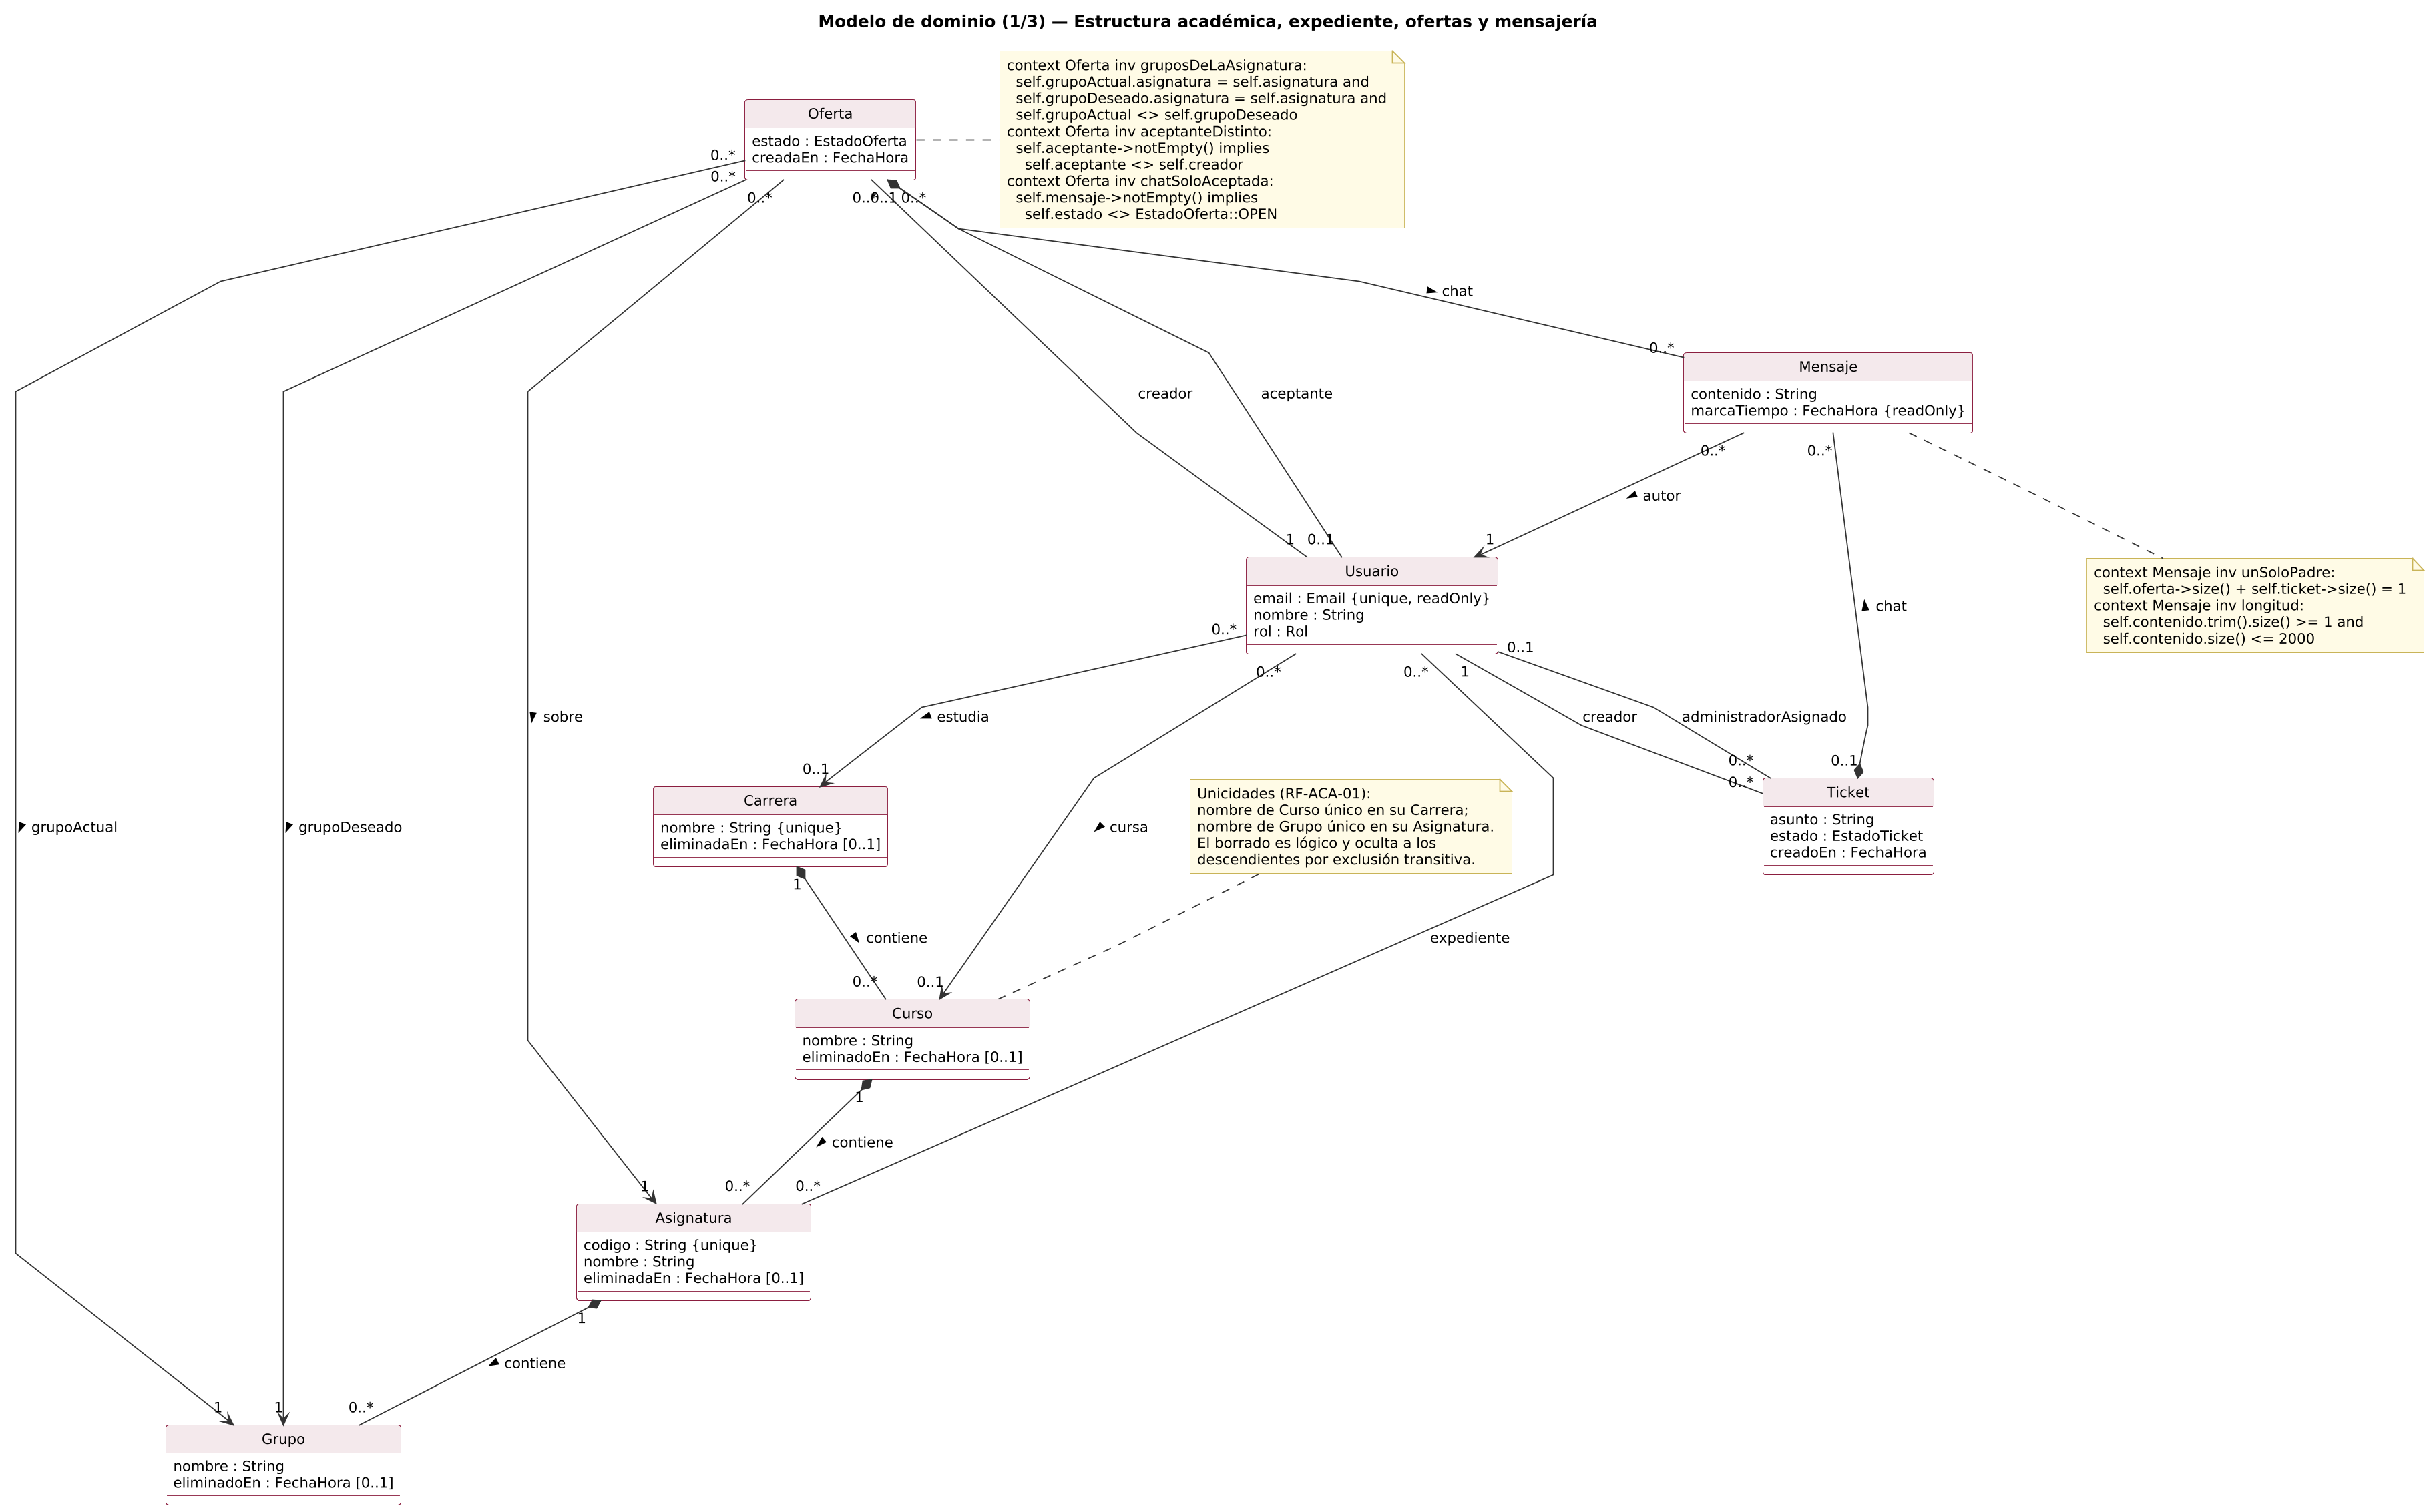
\includegraphics[width=\linewidth,height=0.80\textheight,keepaspectratio]{img/dom01-academico-ofertas.png}\caption{Estructura académica (composición estricta Carrera $\blacklozenge$ Curso $\blacklozenge$ Asignatura $\blacklozenge$ Grupo), expediente, ofertas y mensajería.}\label{fig:dom01-academico-ofertas}\end{figure}

\paragraph{Decisiones de modelado.}
\begin{itemize}[leftmargin=*,itemsep=1pt]
\item La jerarquía académica es \textbf{composición}: un grupo no existe fuera de su asignatura. El borrado es lógico, pero conceptualmente el ciclo de vida de las partes depende del todo (RF-ACA-04).
\item \texttt{Mensaje} es compartido por \texttt{Oferta} y \texttt{Ticket}; UML no puede expresar gráficamente que exactamente uno de los dos sea el todo, así que se declara con OCL (\texttt{unSoloPadre}).
\item El expediente es una asociación muchos a muchos sin atributos propios relevantes, por lo que no se eleva a clase.
\item \texttt{Oferta} se asocia dos veces con \texttt{Grupo} con roles distintos; la pertenencia de ambos a la asignatura de la oferta es una restricción OCL.
\end{itemize}

\begin{figure}[H]\centering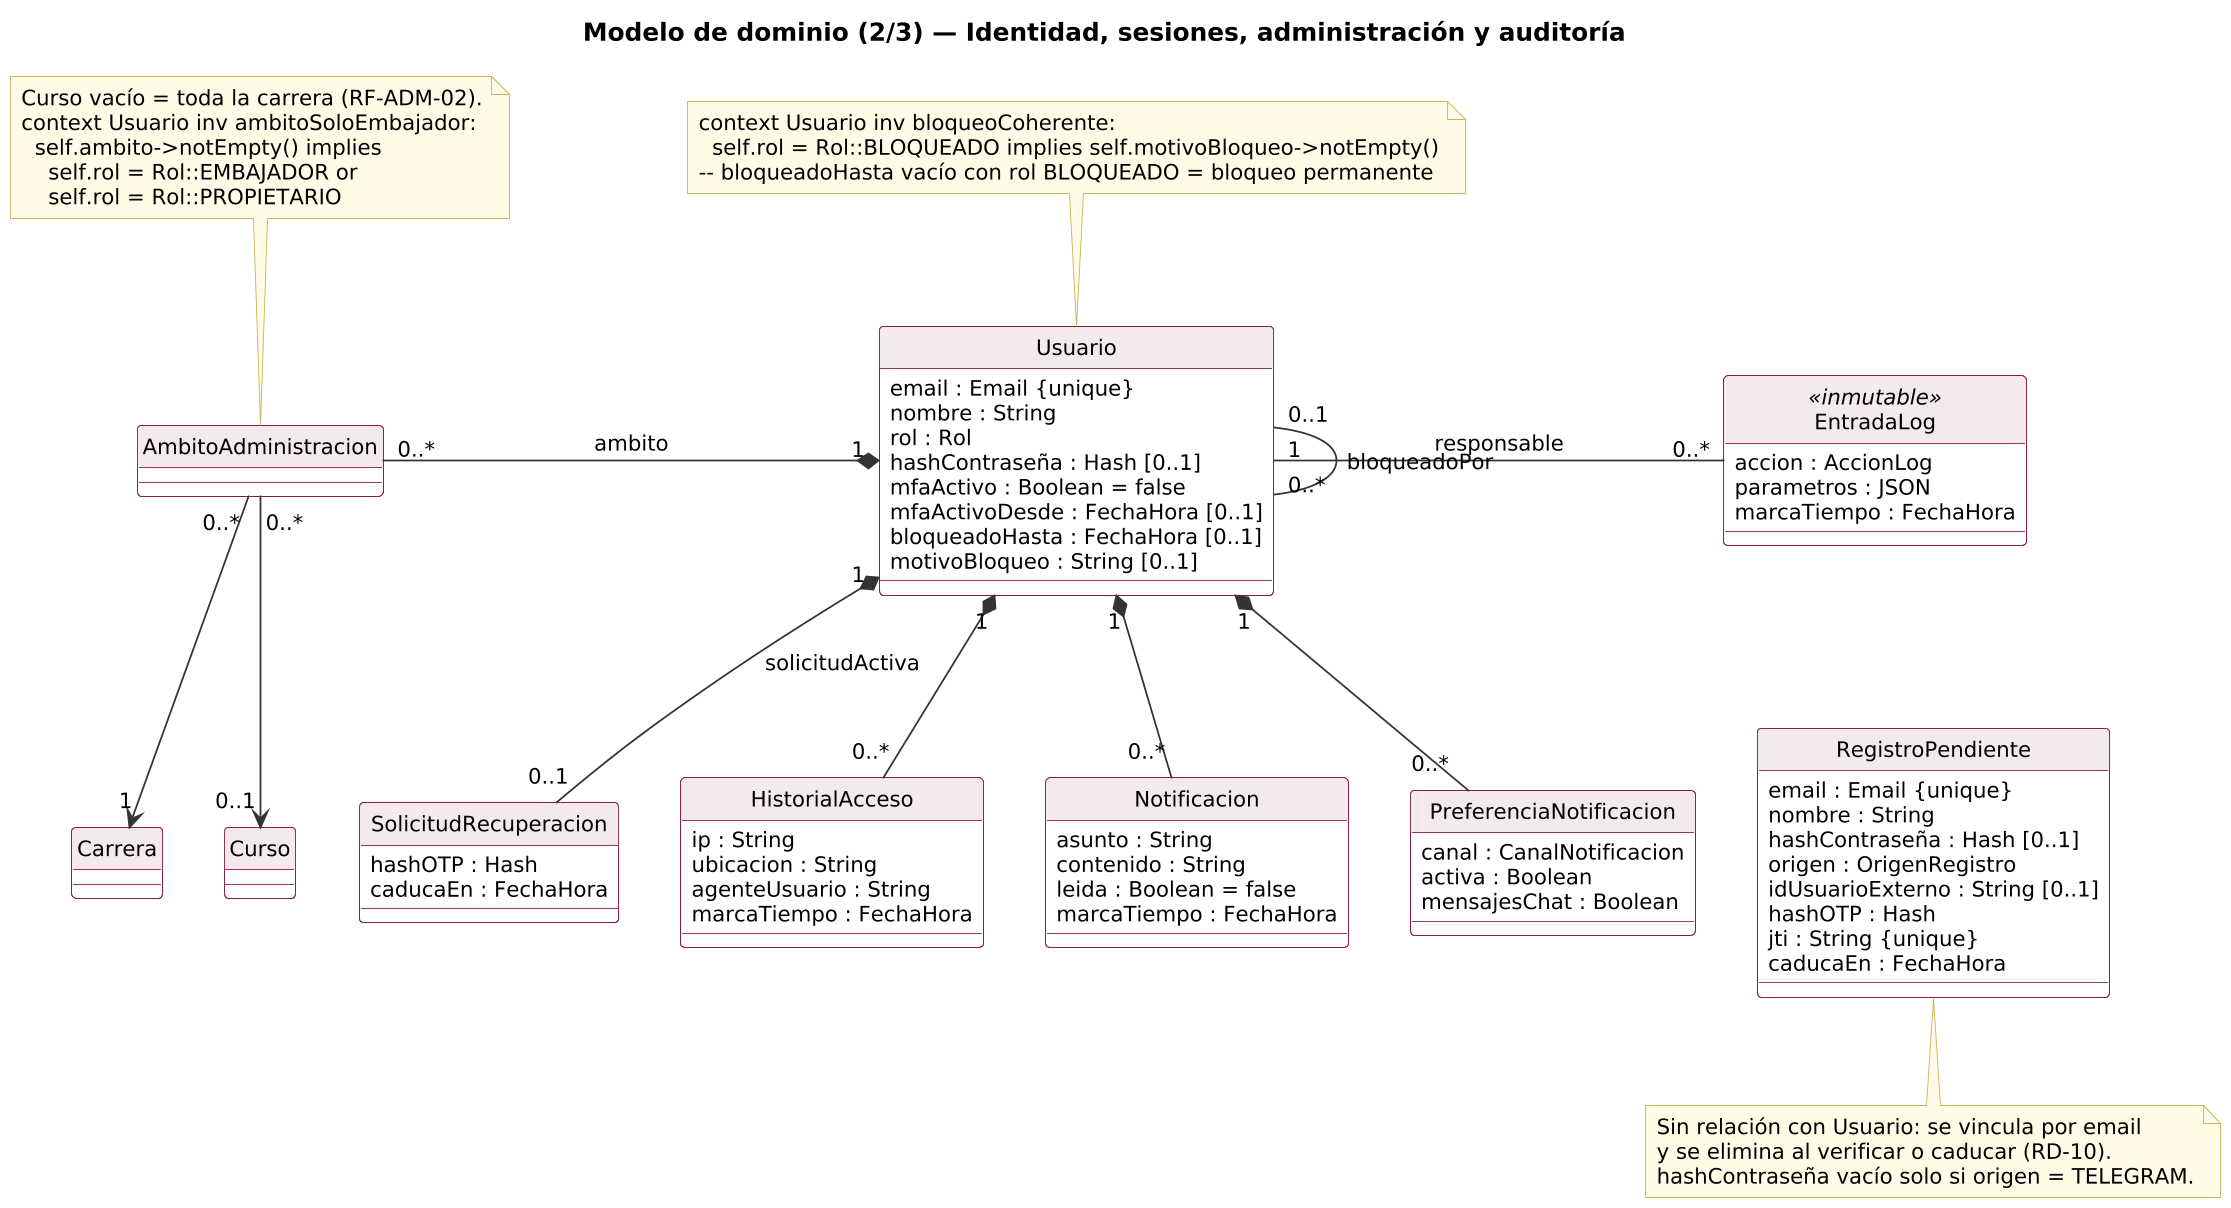
\includegraphics[width=\linewidth,height=0.80\textheight,keepaspectratio]{img/dom02-identidad-seguridad.png}\caption{Identidad, ámbito de administración, notificaciones y auditoría.}\label{fig:dom02-identidad-seguridad}\end{figure}
\begin{figure}[H]\centering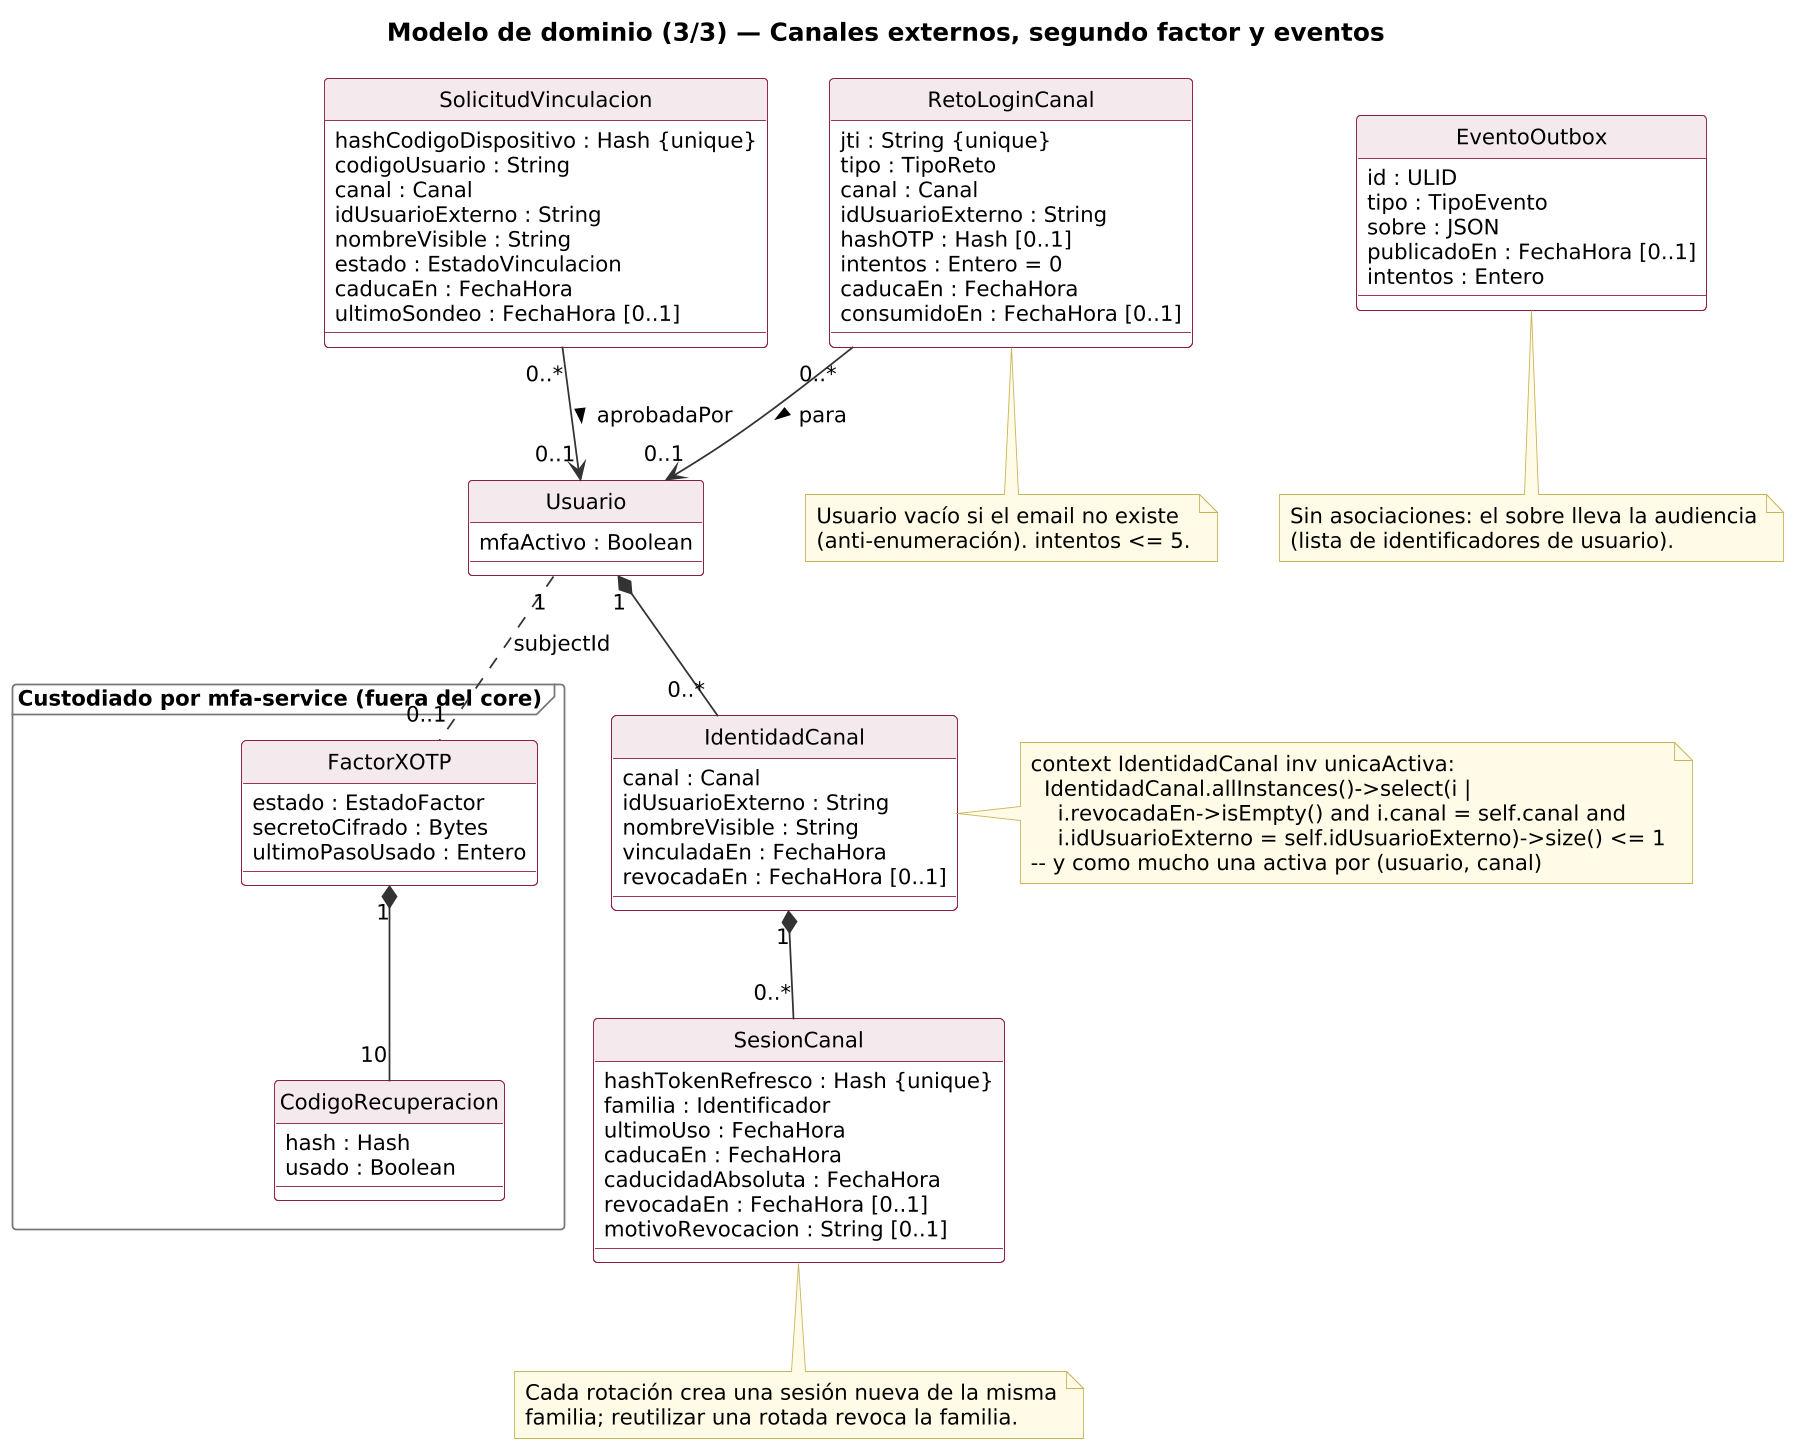
\includegraphics[width=0.92\linewidth,height=0.80\textheight,keepaspectratio]{img/dom03-canales-eventos.png}\caption{Canales externos, retos, eventos y el factor XOTP custodiado por el mfa-service.}\label{fig:dom03-canales-eventos}\end{figure}

\paragraph{Frontera de datos.} El paquete \emph{Custodiado por mfa-service} se muestra por completitud, pero sus clases no pertenecen al sistema de información del core (principio \emph{cada servicio es dueño de sus datos}). El core solo conoce el estado \texttt{mfaActivo} del usuario (ADR-28) y se relaciona con el factor mediante una dependencia por identificador (\texttt{subjectId}).

\begin{figure}[H]\centering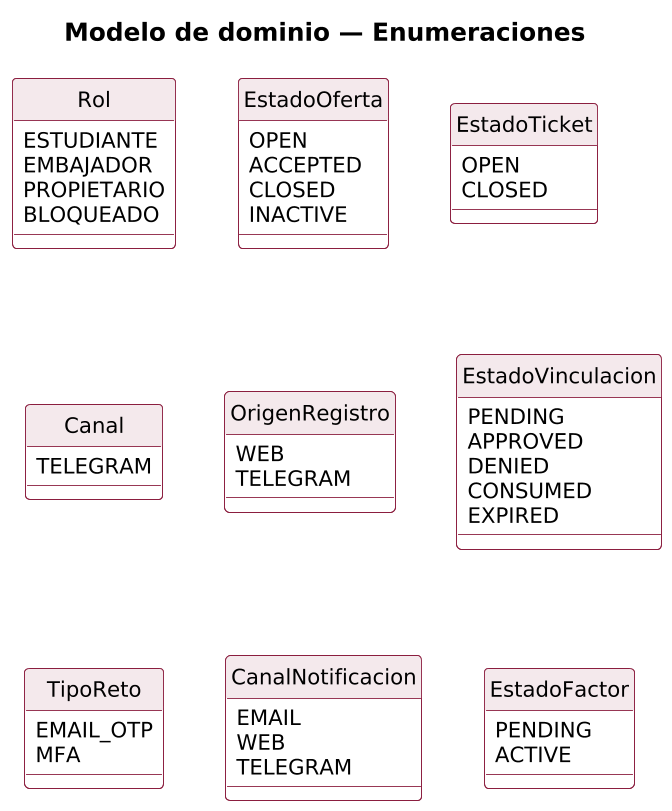
\includegraphics[width=0.45\linewidth,height=0.80\textheight,keepaspectratio]{img/dom04-enumeraciones.png}\caption{Enumeraciones del dominio.}\label{fig:dom04-enumeraciones}\end{figure}
\begin{figure}[H]\centering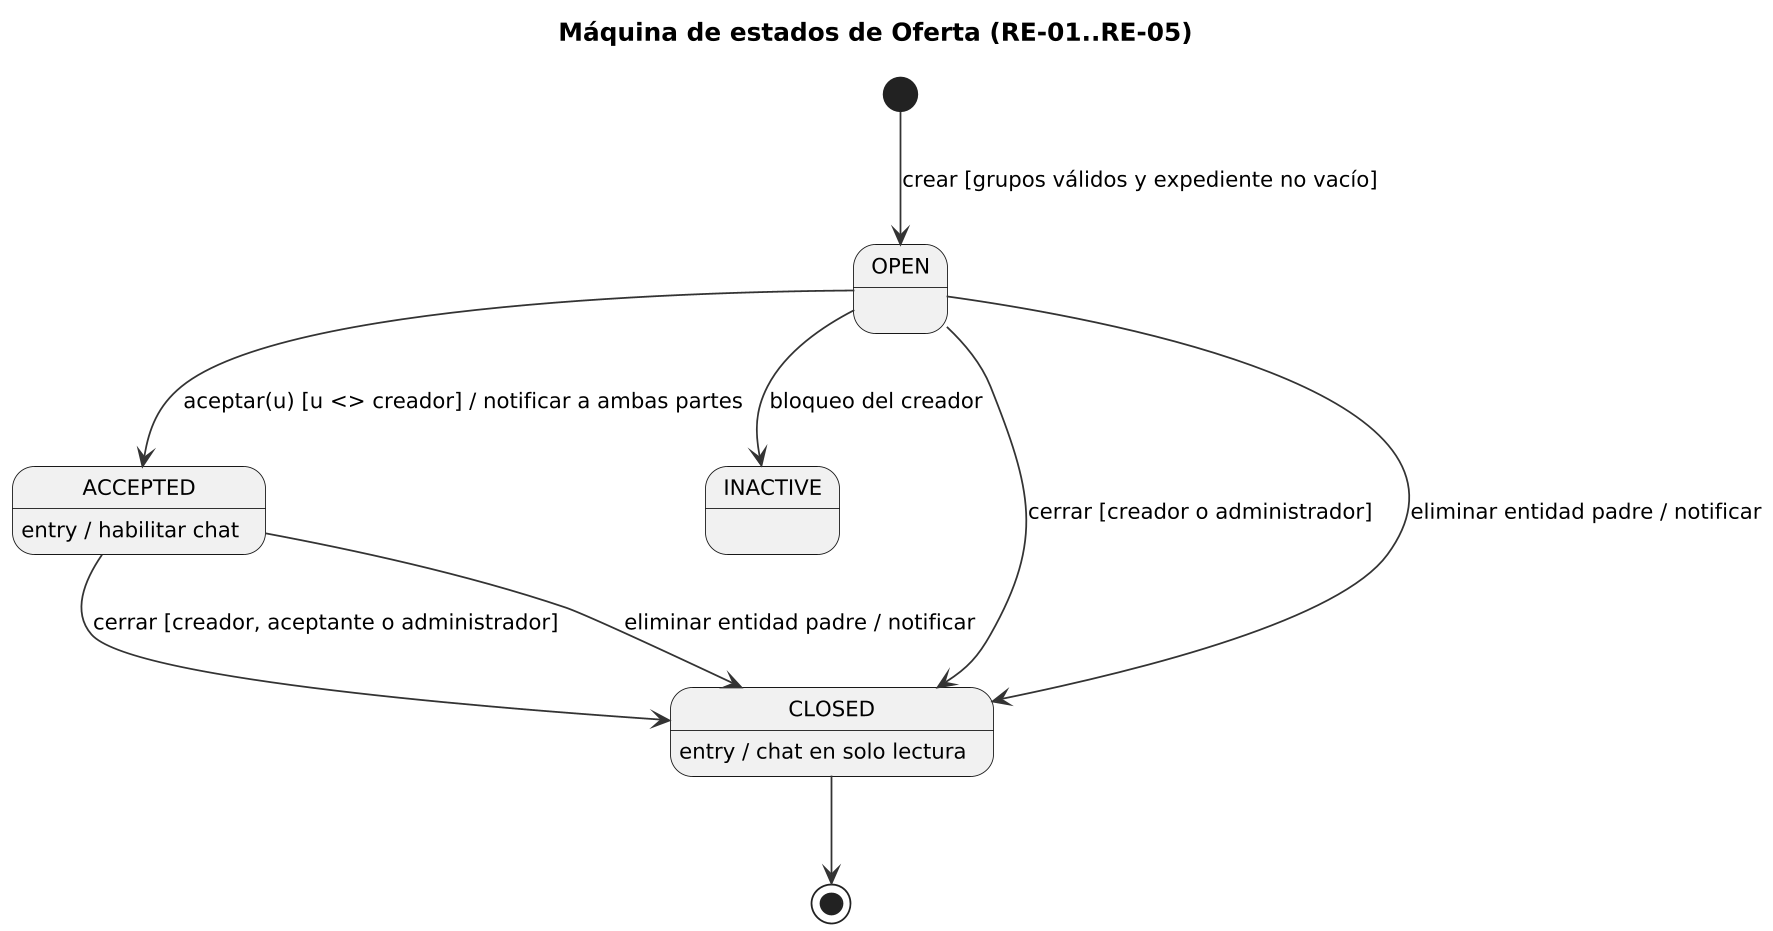
\includegraphics[width=0.85\linewidth,height=0.80\textheight,keepaspectratio]{img/st01-oferta.png}\caption{Máquina de estados del ciclo de vida de una oferta.}\label{fig:st01-oferta}\end{figure}

\section{Modelo de acciones (diagramas de secuencia del sistema)}
Cada diagrama trata xChanger como caja negra y muestra solo los mensajes que cruzan su frontera. Se han elegido los flujos con mayor riesgo funcional o de seguridad.

\begin{figure}[H]\centering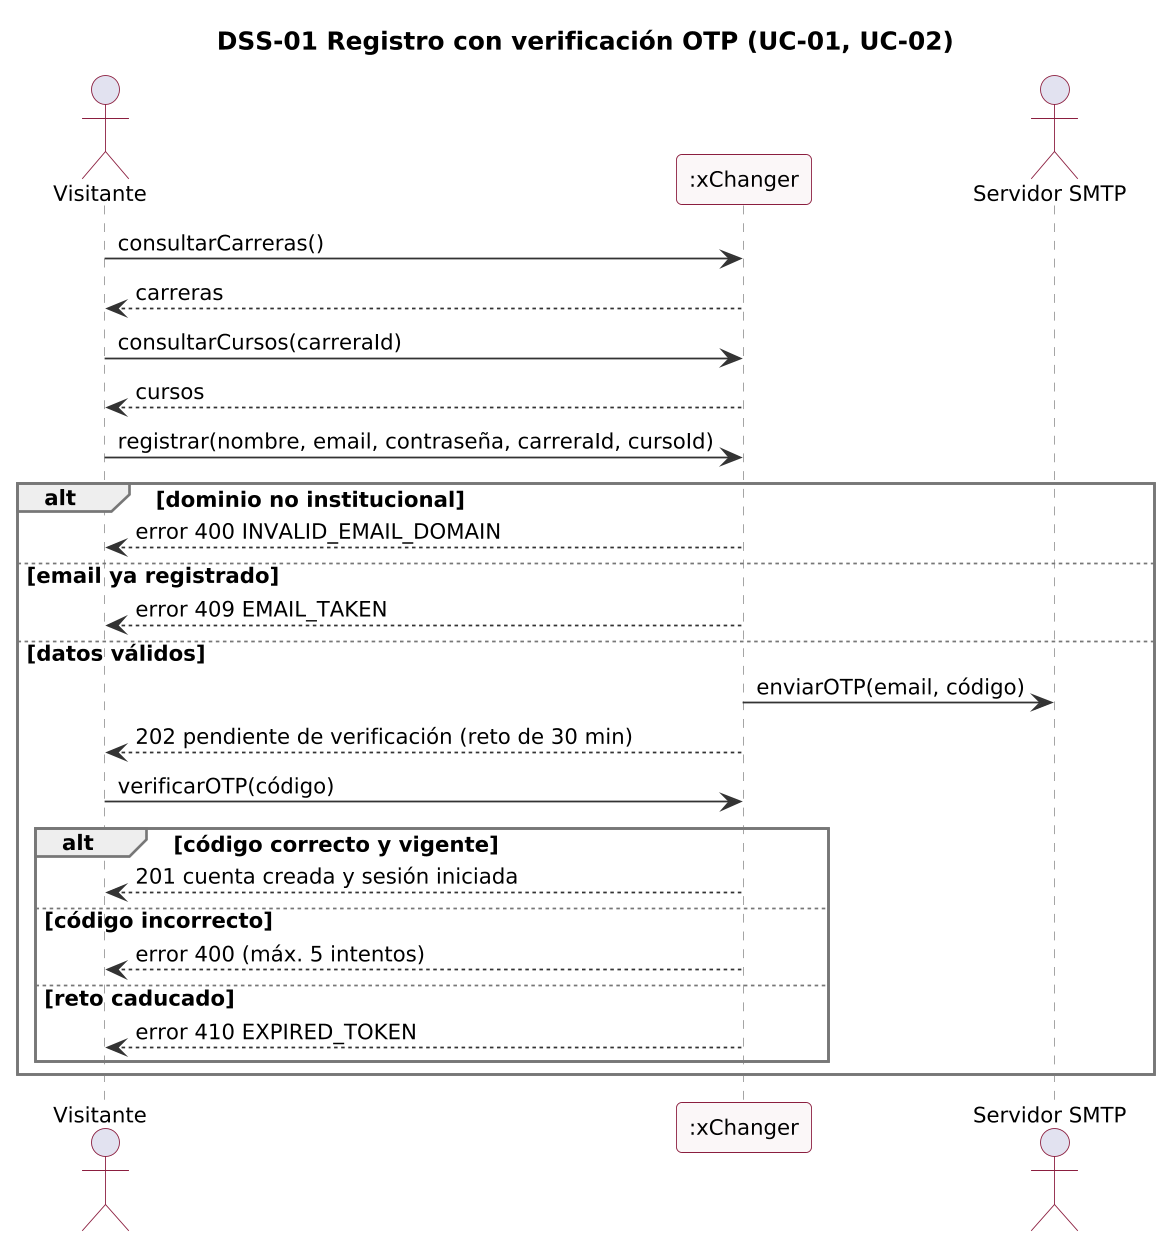
\includegraphics[width=0.72\linewidth,height=0.80\textheight,keepaspectratio]{img/ssd01-registro.png}\caption{DSS-01: registro con verificación OTP.}\label{fig:ssd01-registro}\end{figure}
\begin{figure}[H]\centering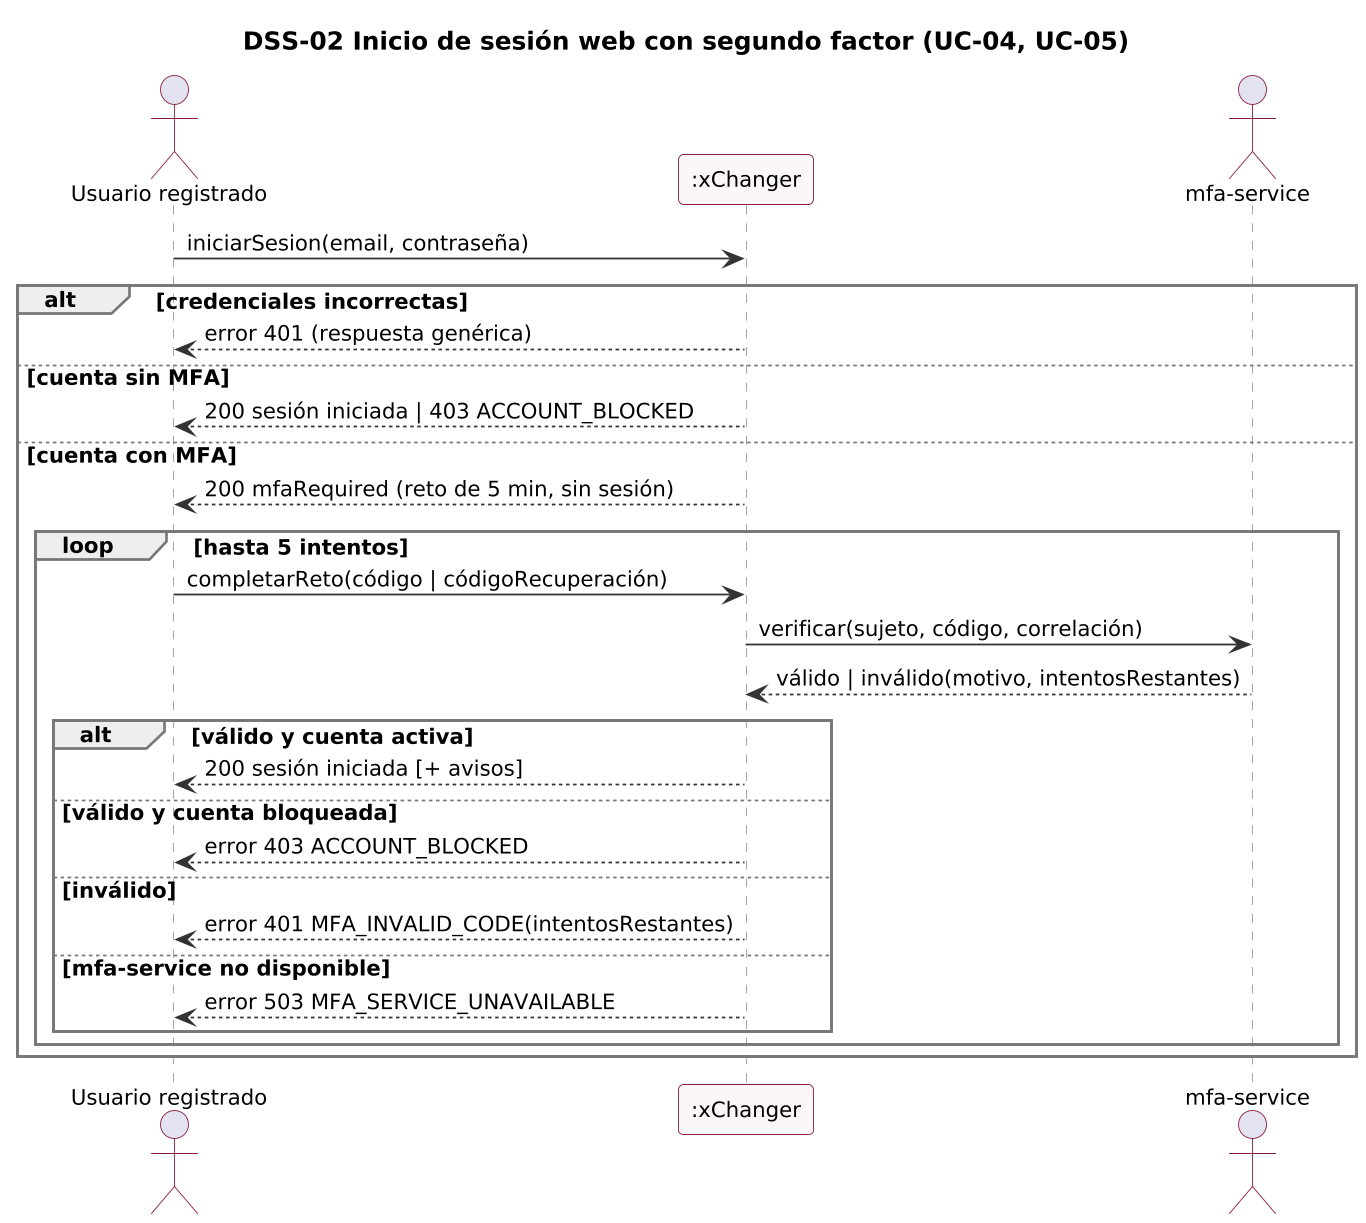
\includegraphics[width=0.80\linewidth,height=0.80\textheight,keepaspectratio]{img/ssd02-login-mfa.png}\caption{DSS-02: inicio de sesión con segundo factor.}\label{fig:ssd02-login-mfa}\end{figure}
\begin{figure}[H]\centering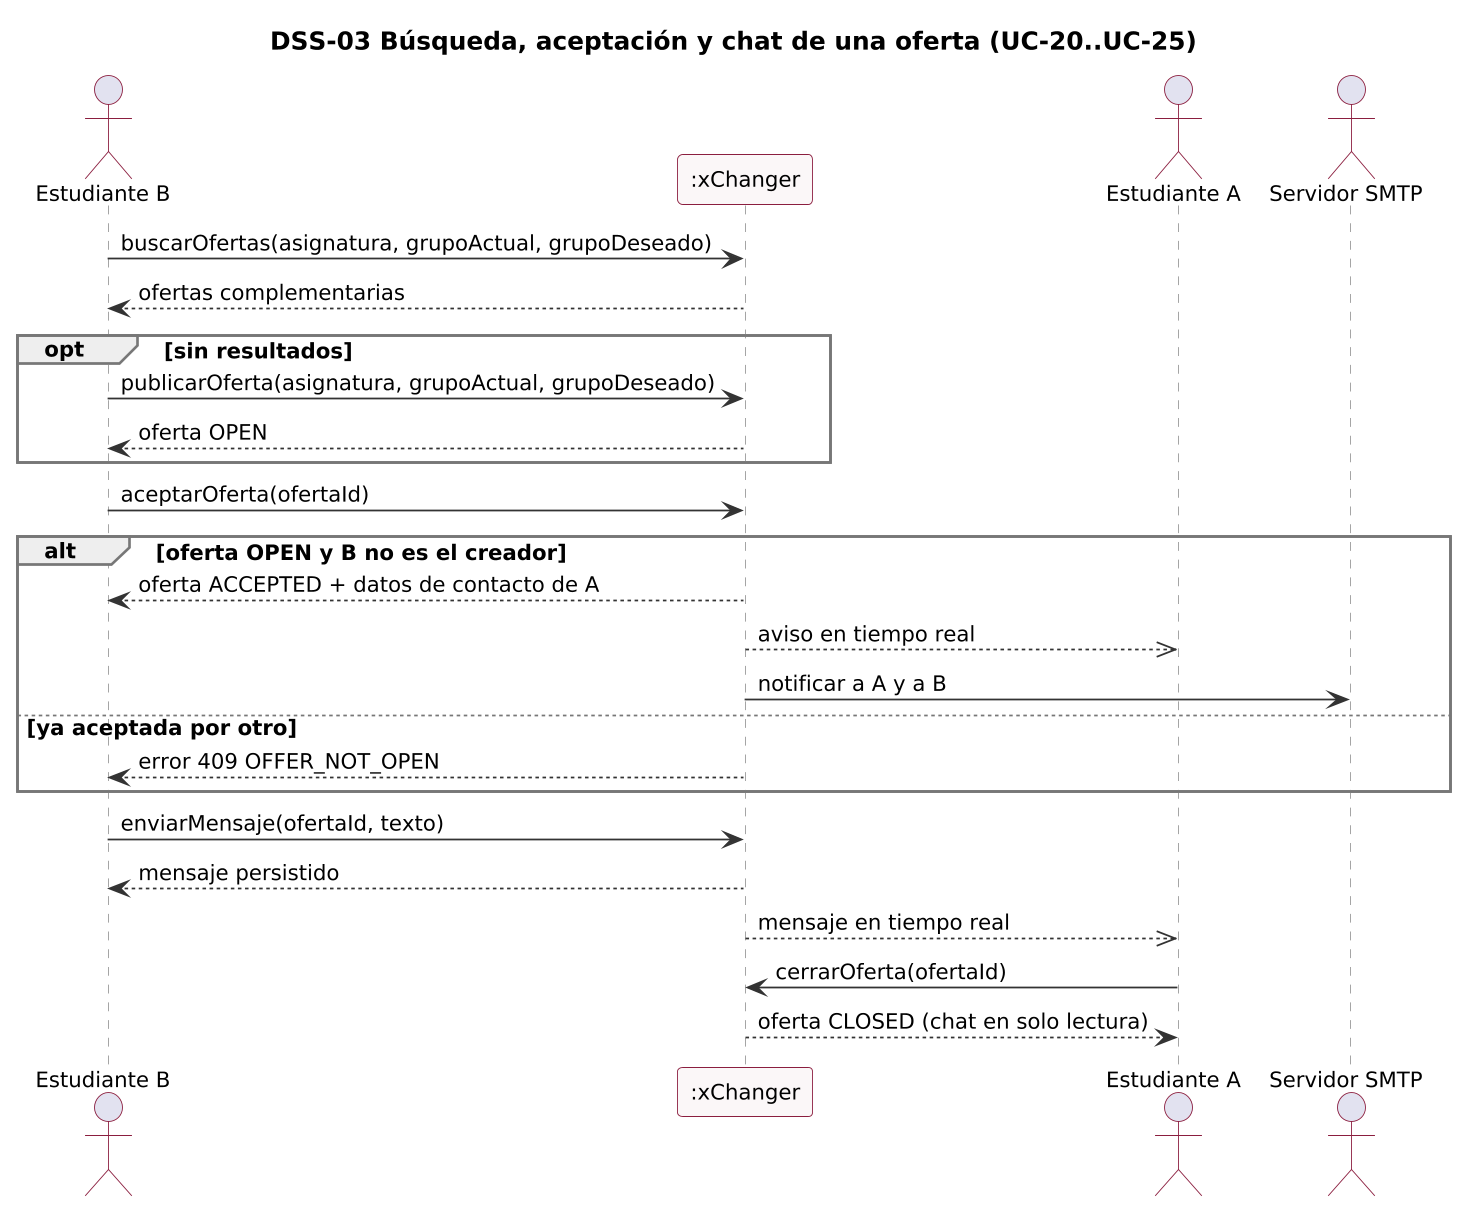
\includegraphics[width=0.82\linewidth,height=0.80\textheight,keepaspectratio]{img/ssd03-intercambio.png}\caption{DSS-03: búsqueda, aceptación y chat de una oferta.}\label{fig:ssd03-intercambio}\end{figure}
\begin{figure}[H]\centering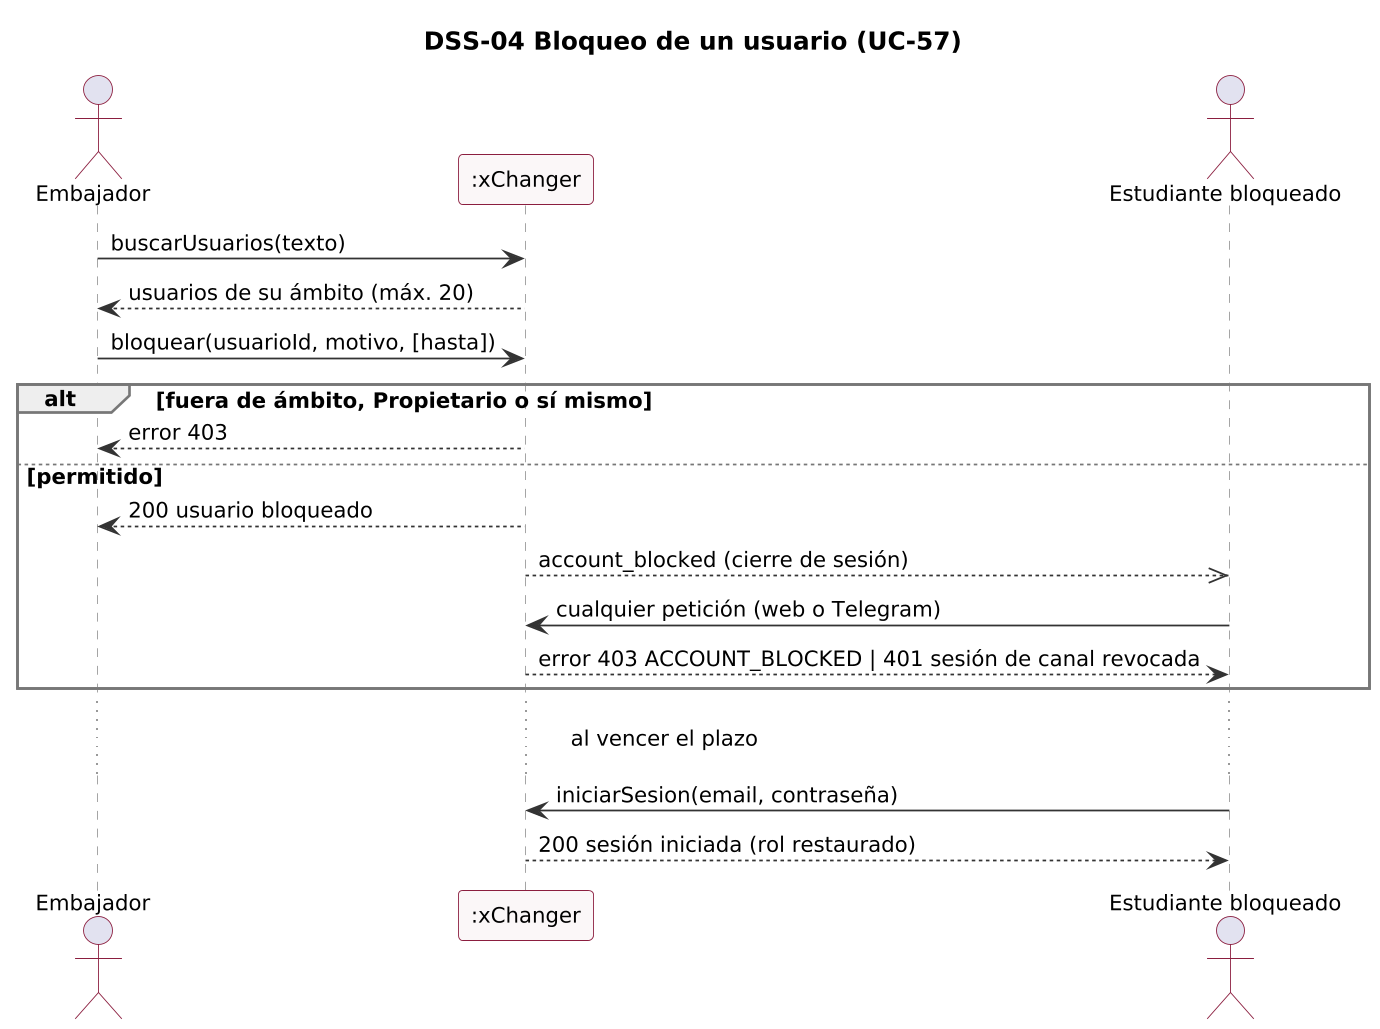
\includegraphics[width=0.80\linewidth,height=0.80\textheight,keepaspectratio]{img/ssd04-bloqueo.png}\caption{DSS-04: bloqueo de un usuario y su efecto inmediato.}\label{fig:ssd04-bloqueo}\end{figure}
\begin{figure}[H]\centering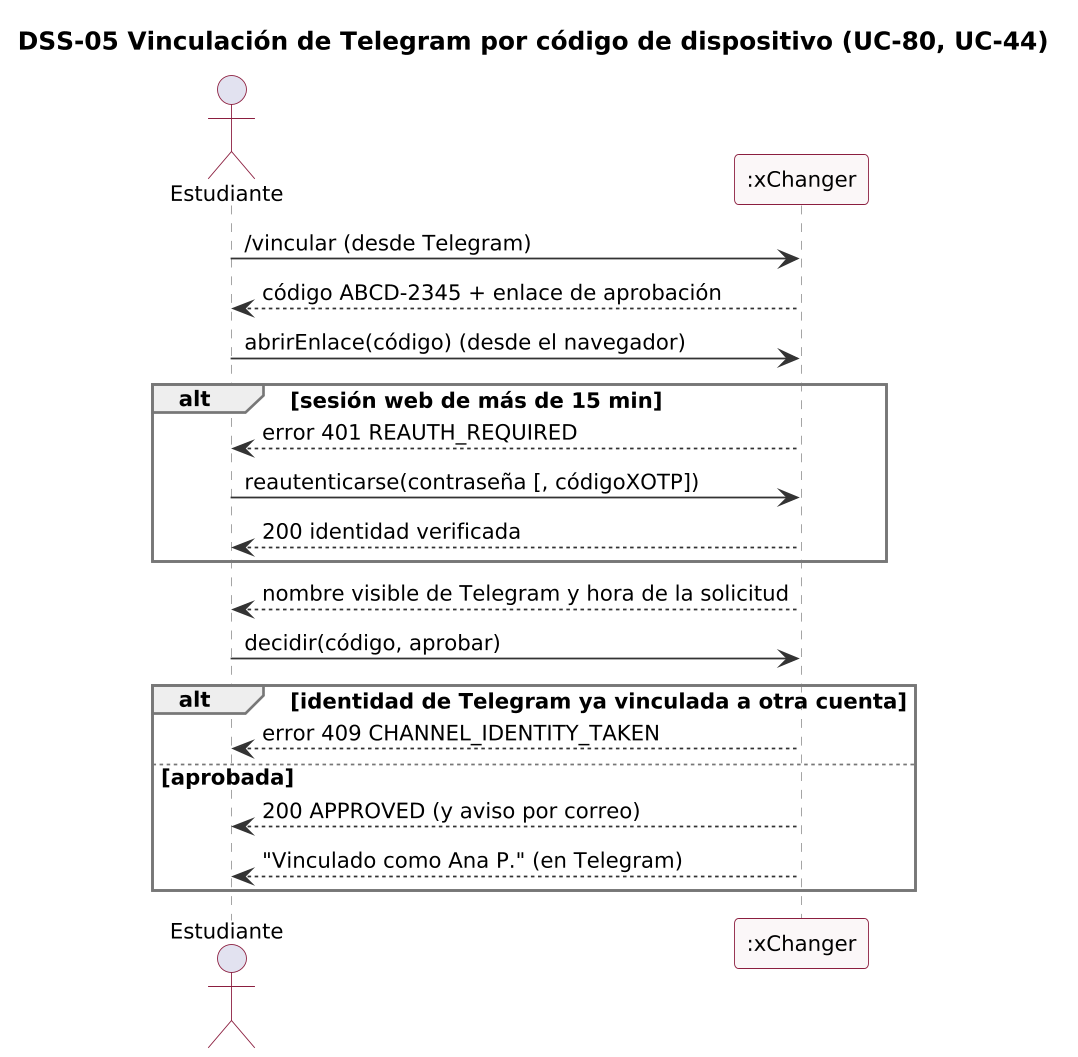
\includegraphics[width=0.70\linewidth,height=0.80\textheight,keepaspectratio]{img/ssd05-vinculacion.png}\caption{DSS-05: vinculación de Telegram por código de dispositivo.}\label{fig:ssd05-vinculacion}\end{figure}
\begin{figure}[H]\centering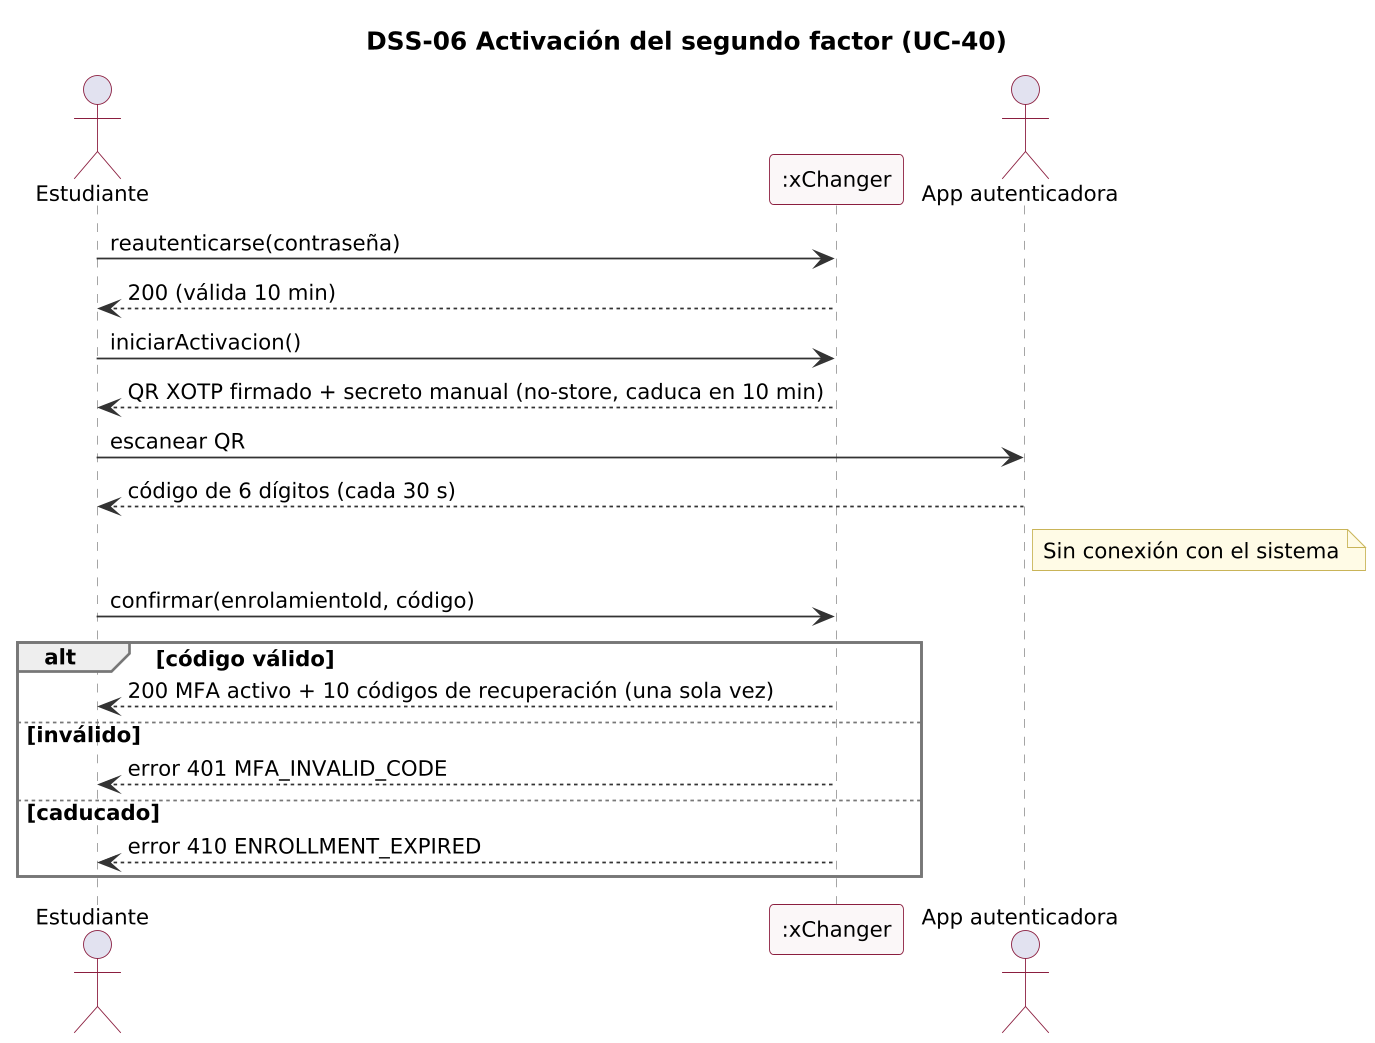
\includegraphics[width=0.80\linewidth,height=0.80\textheight,keepaspectratio]{img/ssd06-activar-mfa.png}\caption{DSS-06: activación del segundo factor.}\label{fig:ssd06-activar-mfa}\end{figure}

%════════════════════════════════════════════════════════════════════
\chapter{Arquitectura del sistema}

\section{Modelo de componentes}
\begin{figure}[H]\centering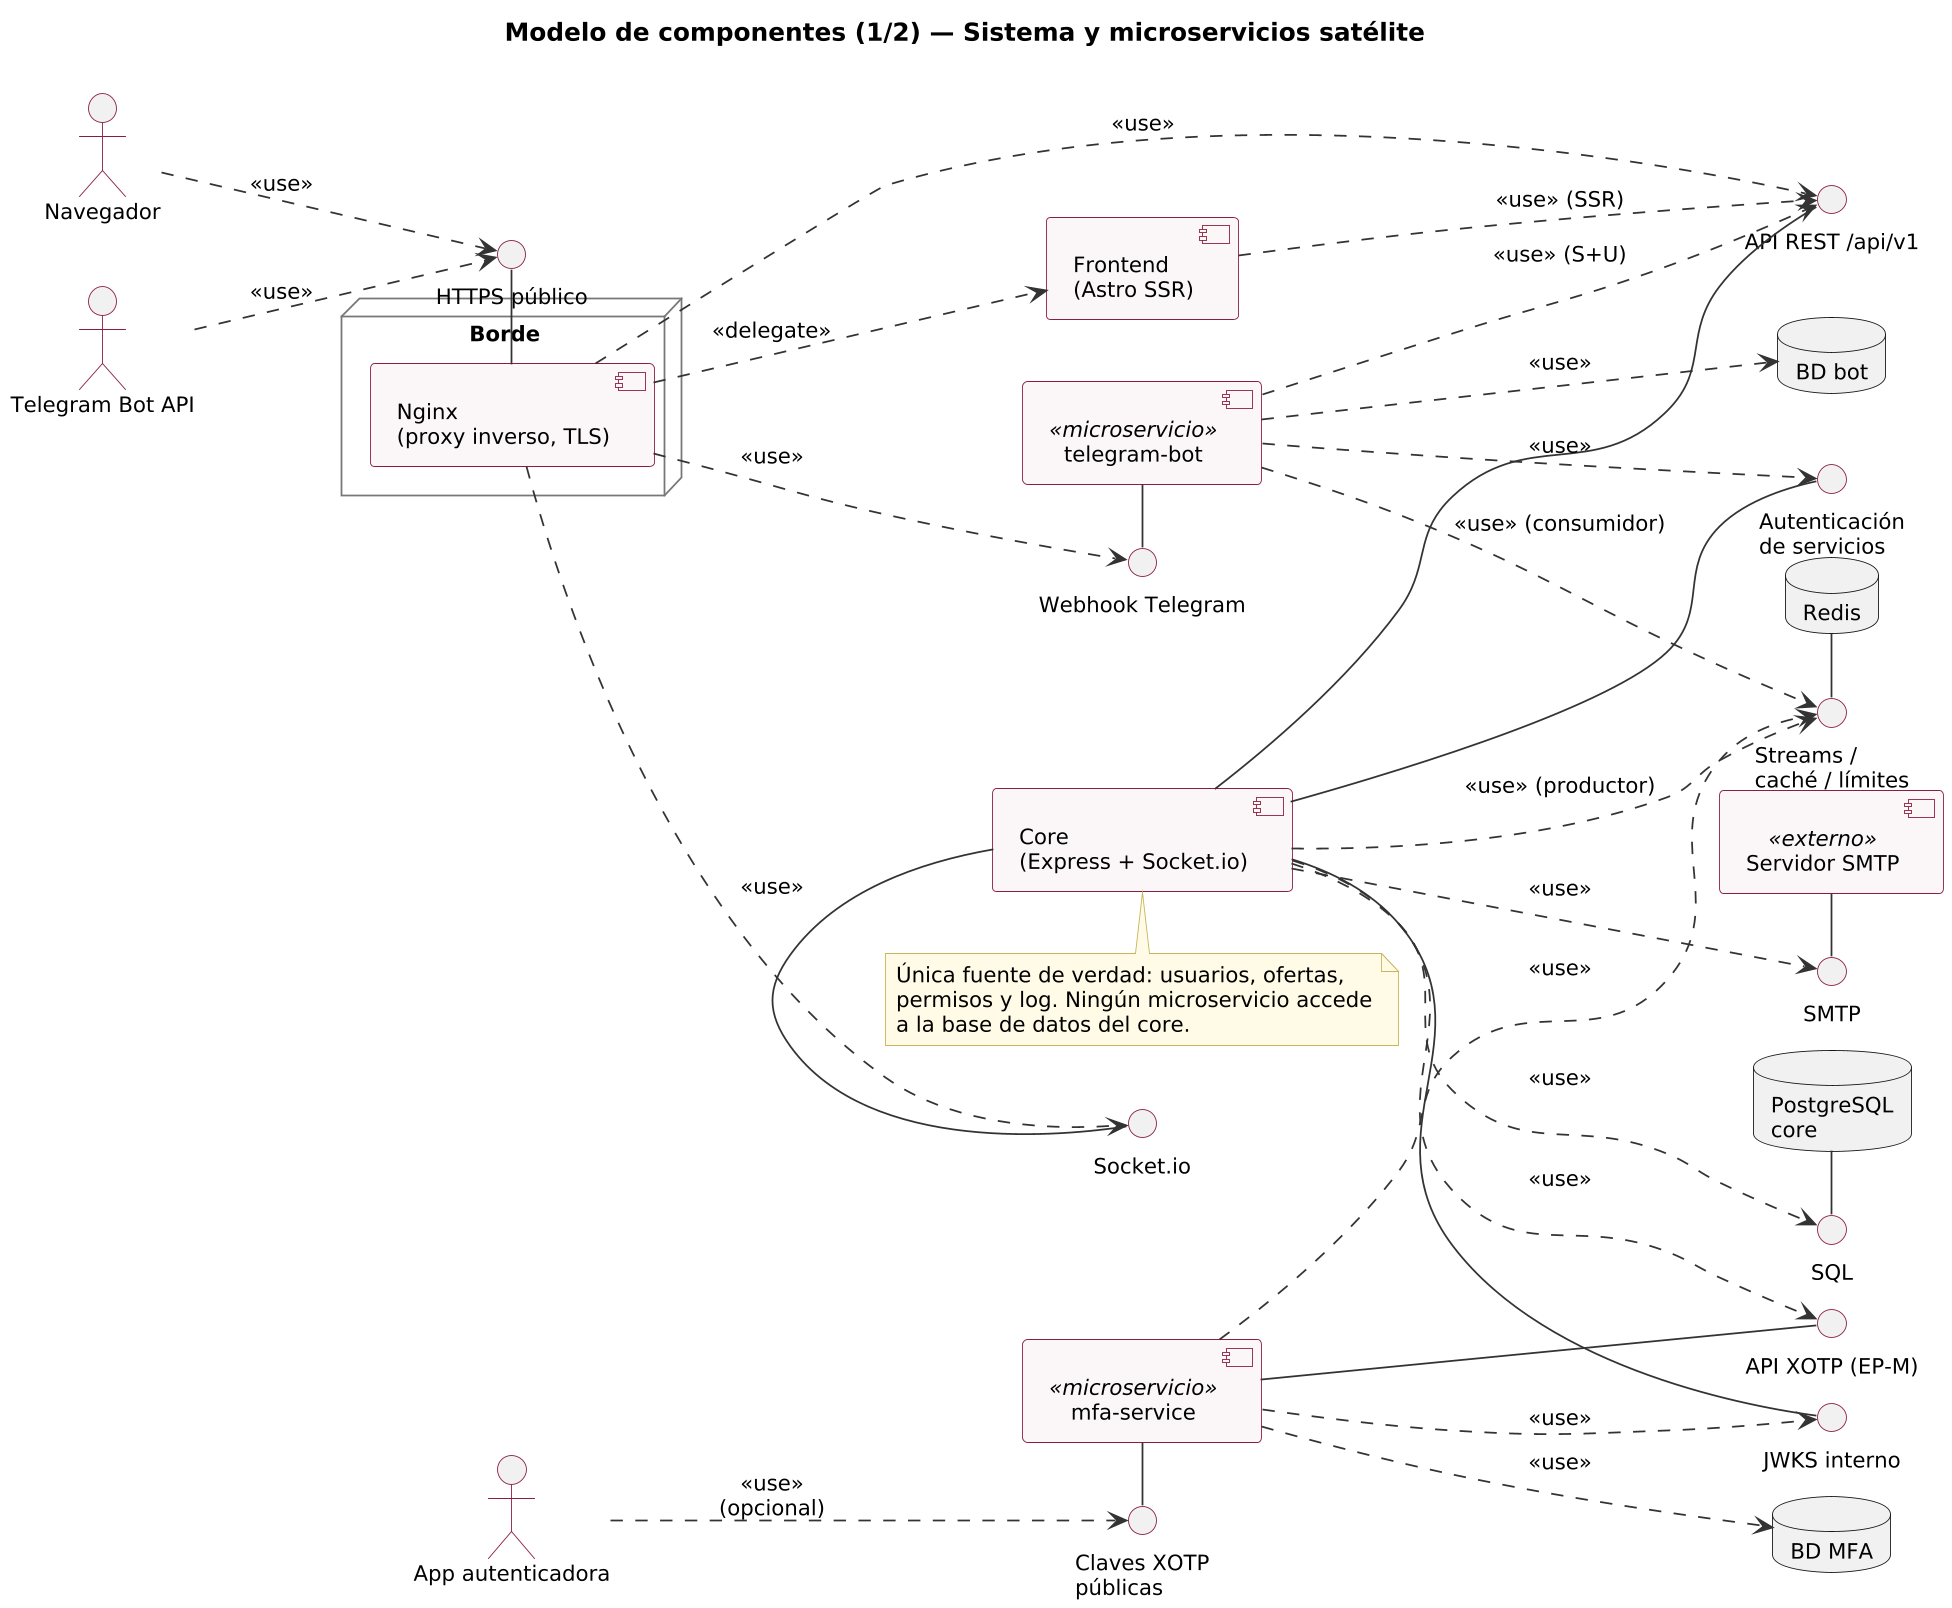
\includegraphics[width=\linewidth,height=0.80\textheight,keepaspectratio]{img/comp01-sistema.png}\caption{Componentes del sistema, interfaces proporcionadas y requeridas.}\label{fig:comp01-sistema}\end{figure}

\begin{center}\small
\begin{tabularx}{\linewidth}{@{}p{3.4cm}p{3.2cm}X@{}}
\toprule
Interfaz & Proveedor & Consumidores y contrato \\
\midrule
API REST \texttt{/api/v1} & Core & Frontend (navegador y SSR), telegram-bot (S+U). Capítulo~\ref{cap:api}. \\
Socket.io & Core & Navegador: salas \texttt{user:}, \texttt{offer:}, \texttt{ticket:} (RE-WS). \\
Autenticación de servicios & Core & telegram-bot: \texttt{client\_credentials} → JWT ES256. \\
JWKS interno & Core & mfa-service: valida los JWT del core. \\
Streams & Redis & Core (productor del outbox), bot y consumidores internos (grupos de consumo). \\
API XOTP (EP-M) & mfa-service & Core: enrolar, verificar, recuperar, revocar. \\
Webhook Telegram & telegram-bot & Telegram Bot API, a través de Nginx. \\
\bottomrule
\end{tabularx}
\end{center}

\begin{figure}[H]\centering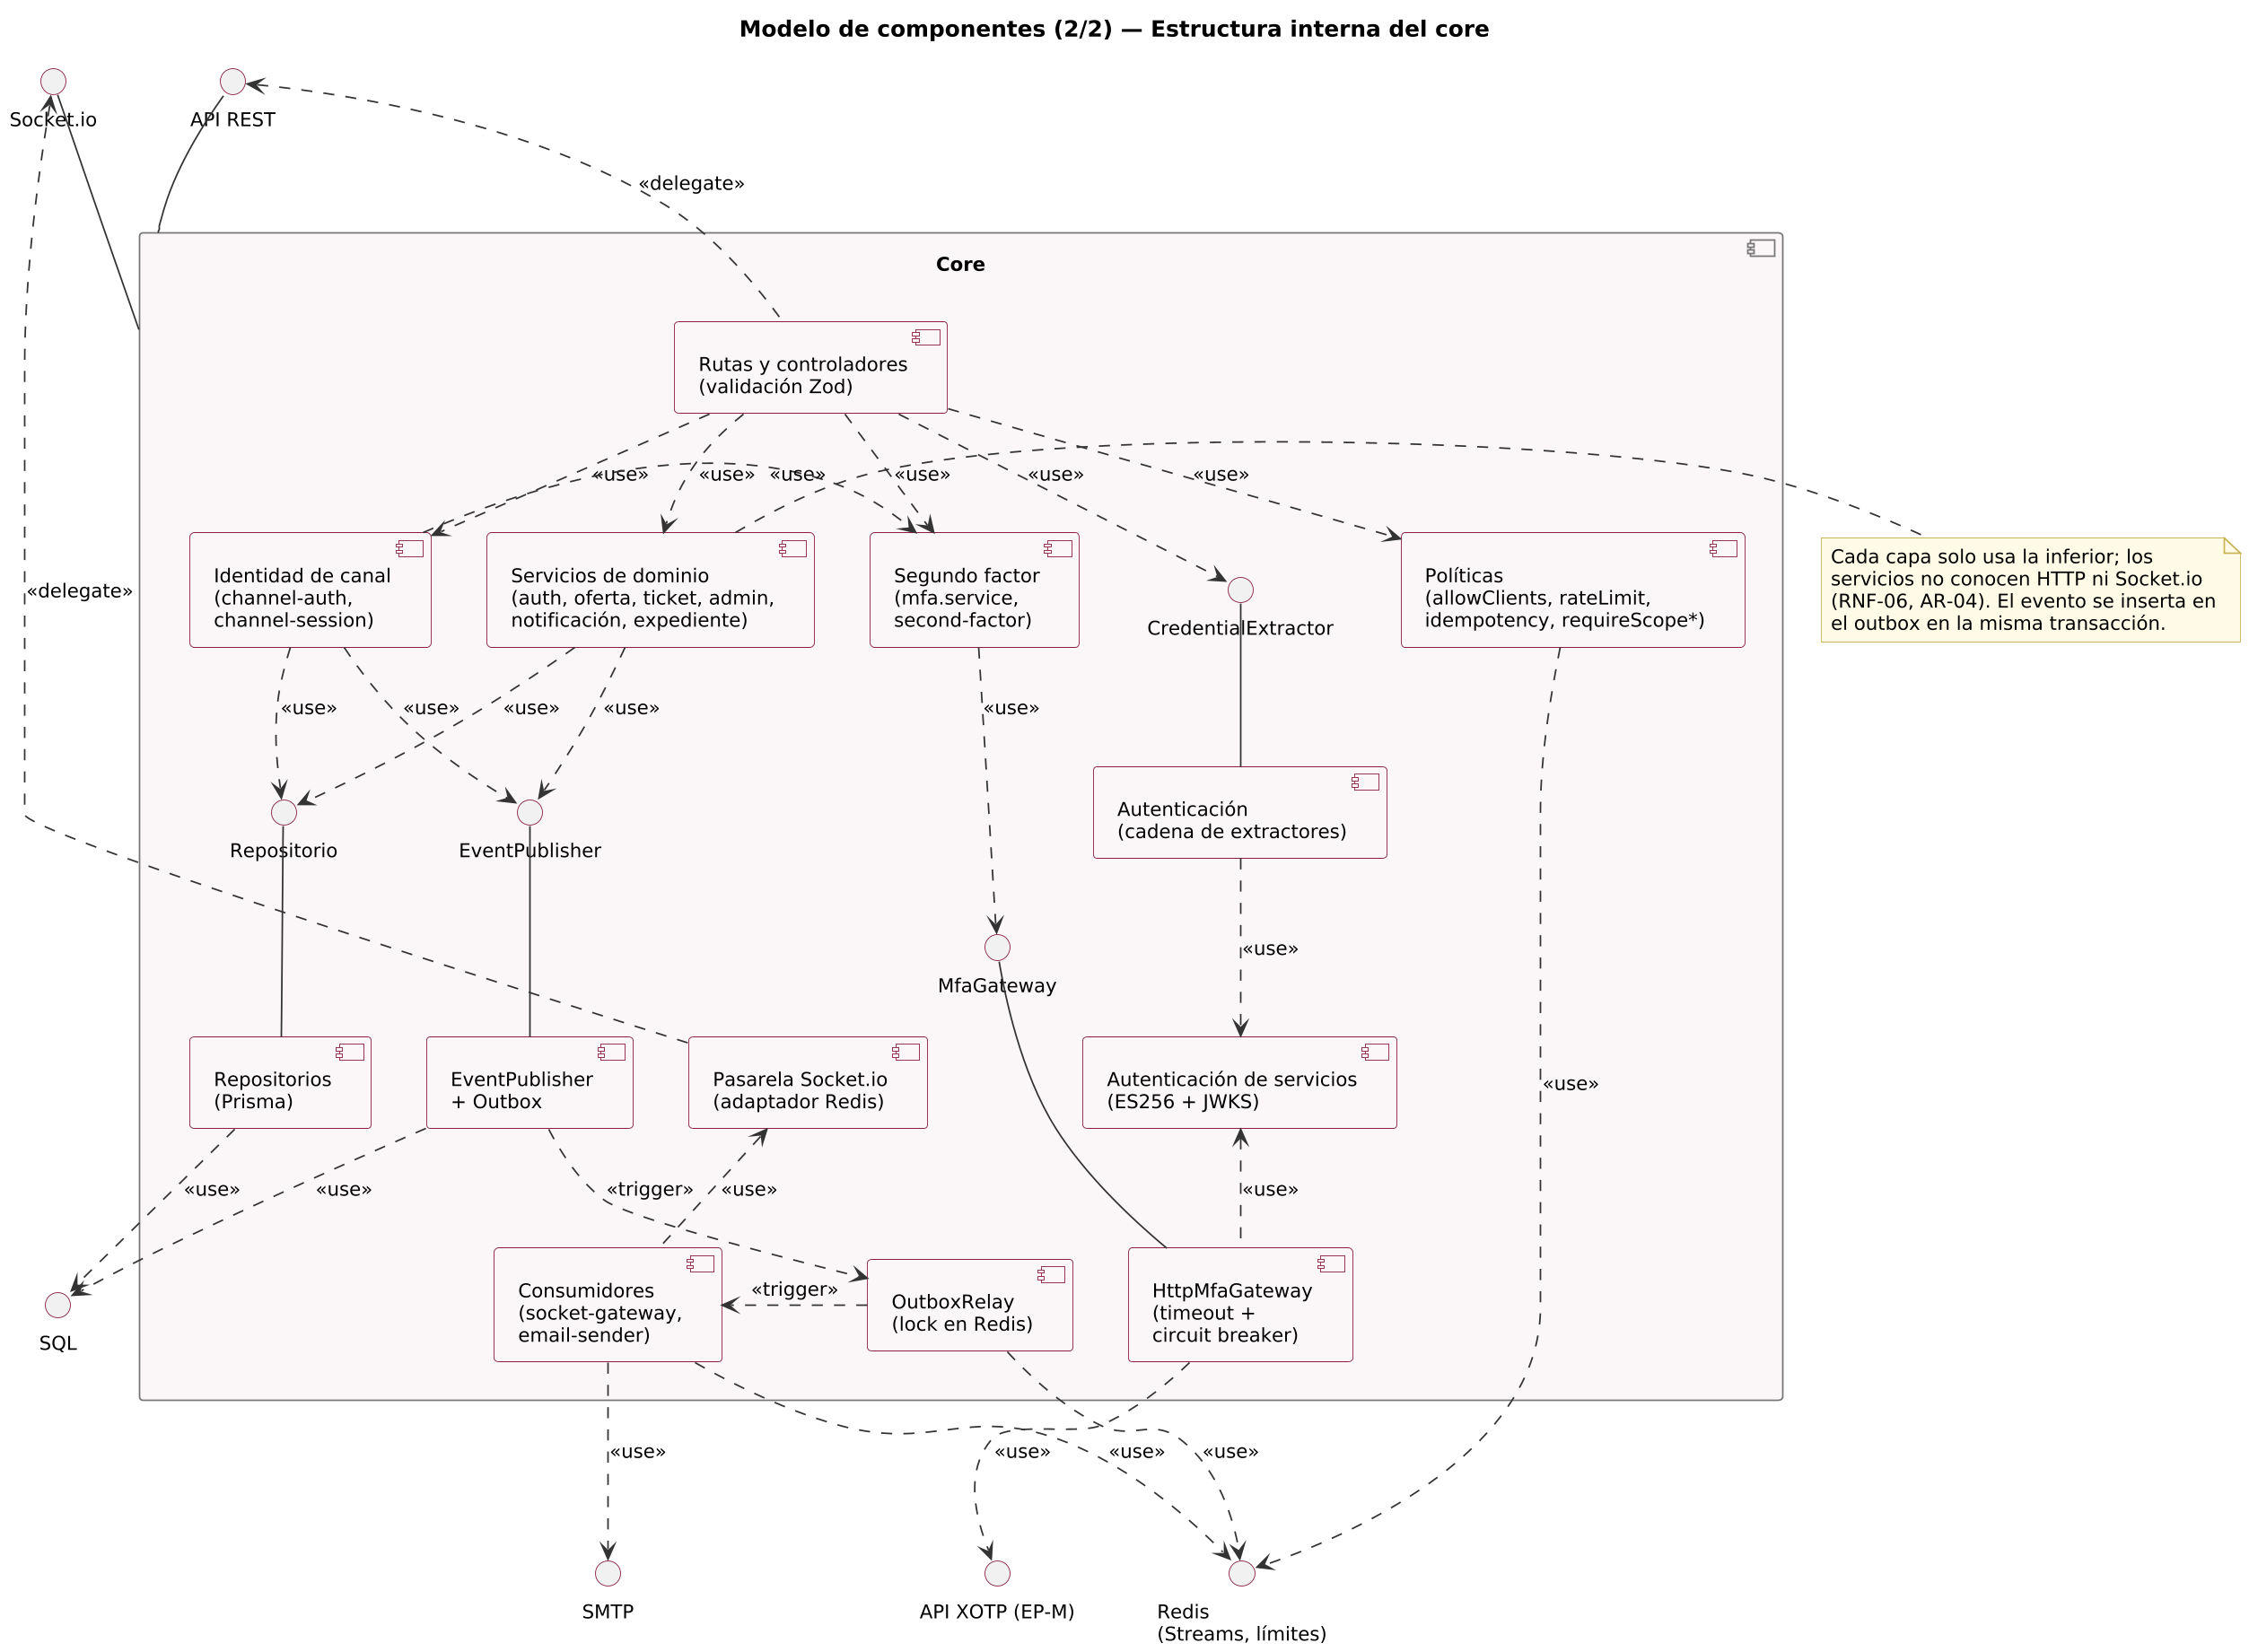
\includegraphics[width=\linewidth,height=0.80\textheight,keepaspectratio]{img/comp02-core.png}\caption{Estructura interna del core por capas.}\label{fig:comp02-core}\end{figure}

\paragraph{Reglas de dependencia.} Las flechas \guillemotleft use\guillemotright{} solo descienden de capa. Los servicios dependen de las interfaces \texttt{Repositorio}, \texttt{EventPublisher} y \texttt{MfaGateway}, no de sus implementaciones; esto permite sustituir el cliente del mfa-service por un doble en las pruebas y que ningún servicio conozca Socket.io (AR-04).

\section{Interacción de componentes}
\begin{sidewaysfigure}\centering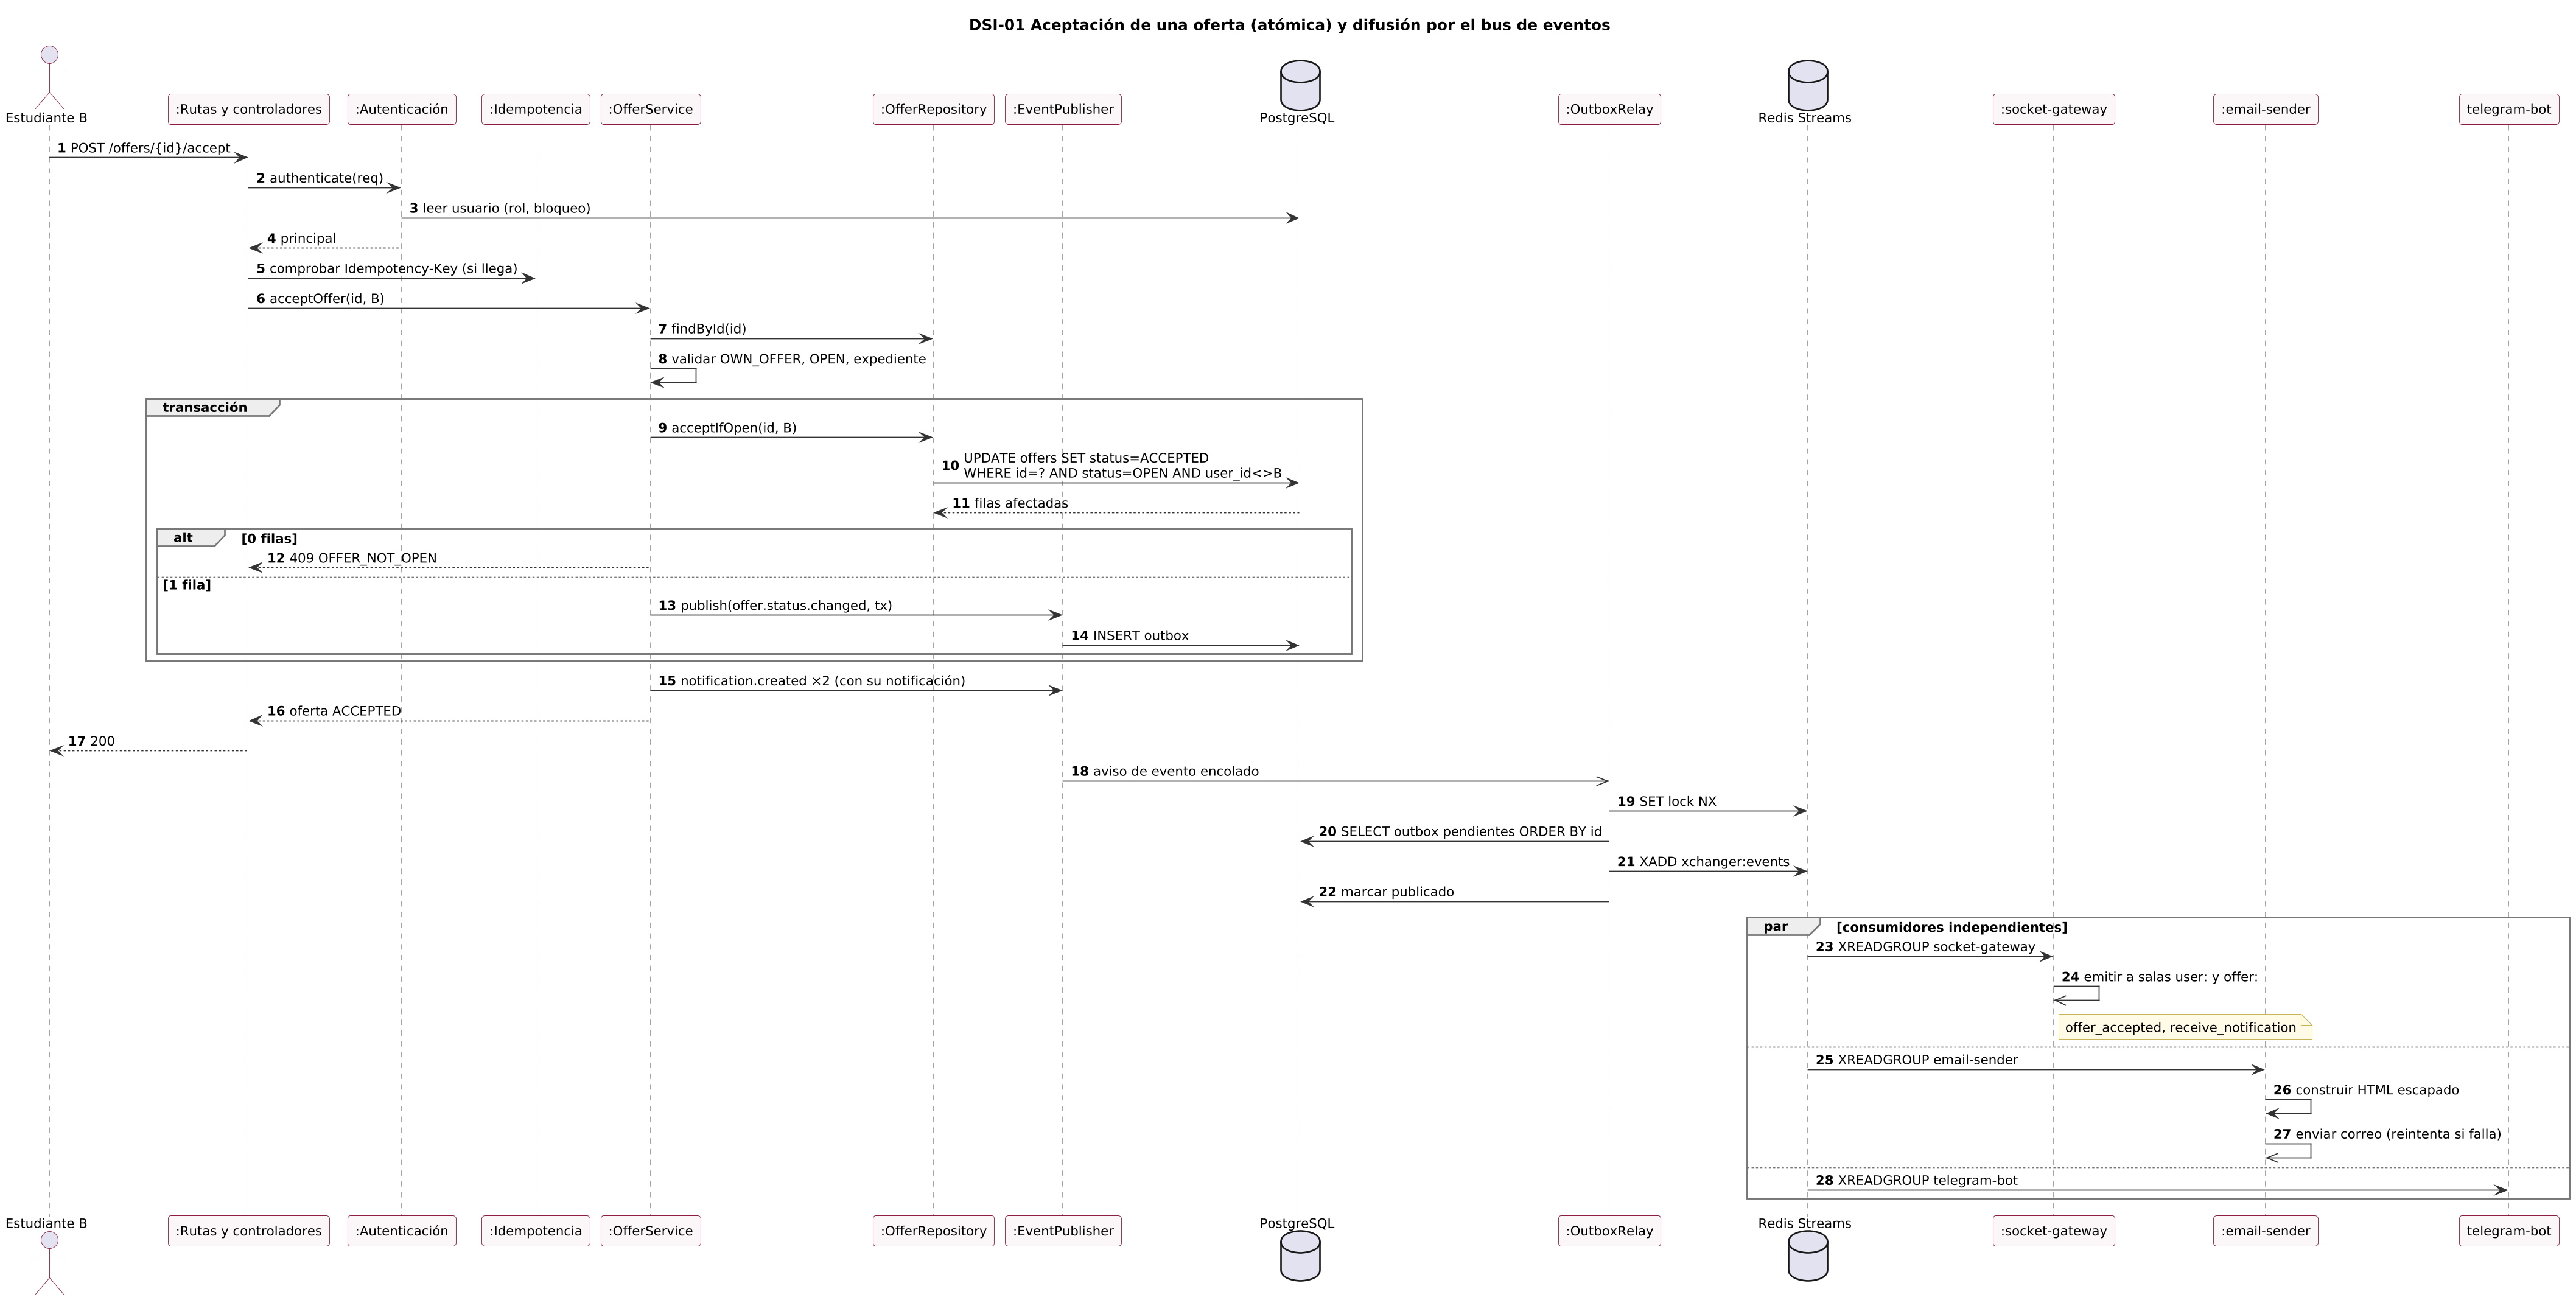
\includegraphics[width=\textheight,height=0.85\textwidth,keepaspectratio]{img/seq01-aceptar-oferta.png}\caption{DSI-01: aceptación atómica de una oferta y difusión por el bus de eventos.}\label{fig:seq01-aceptar-oferta}\end{sidewaysfigure}
\begin{sidewaysfigure}\centering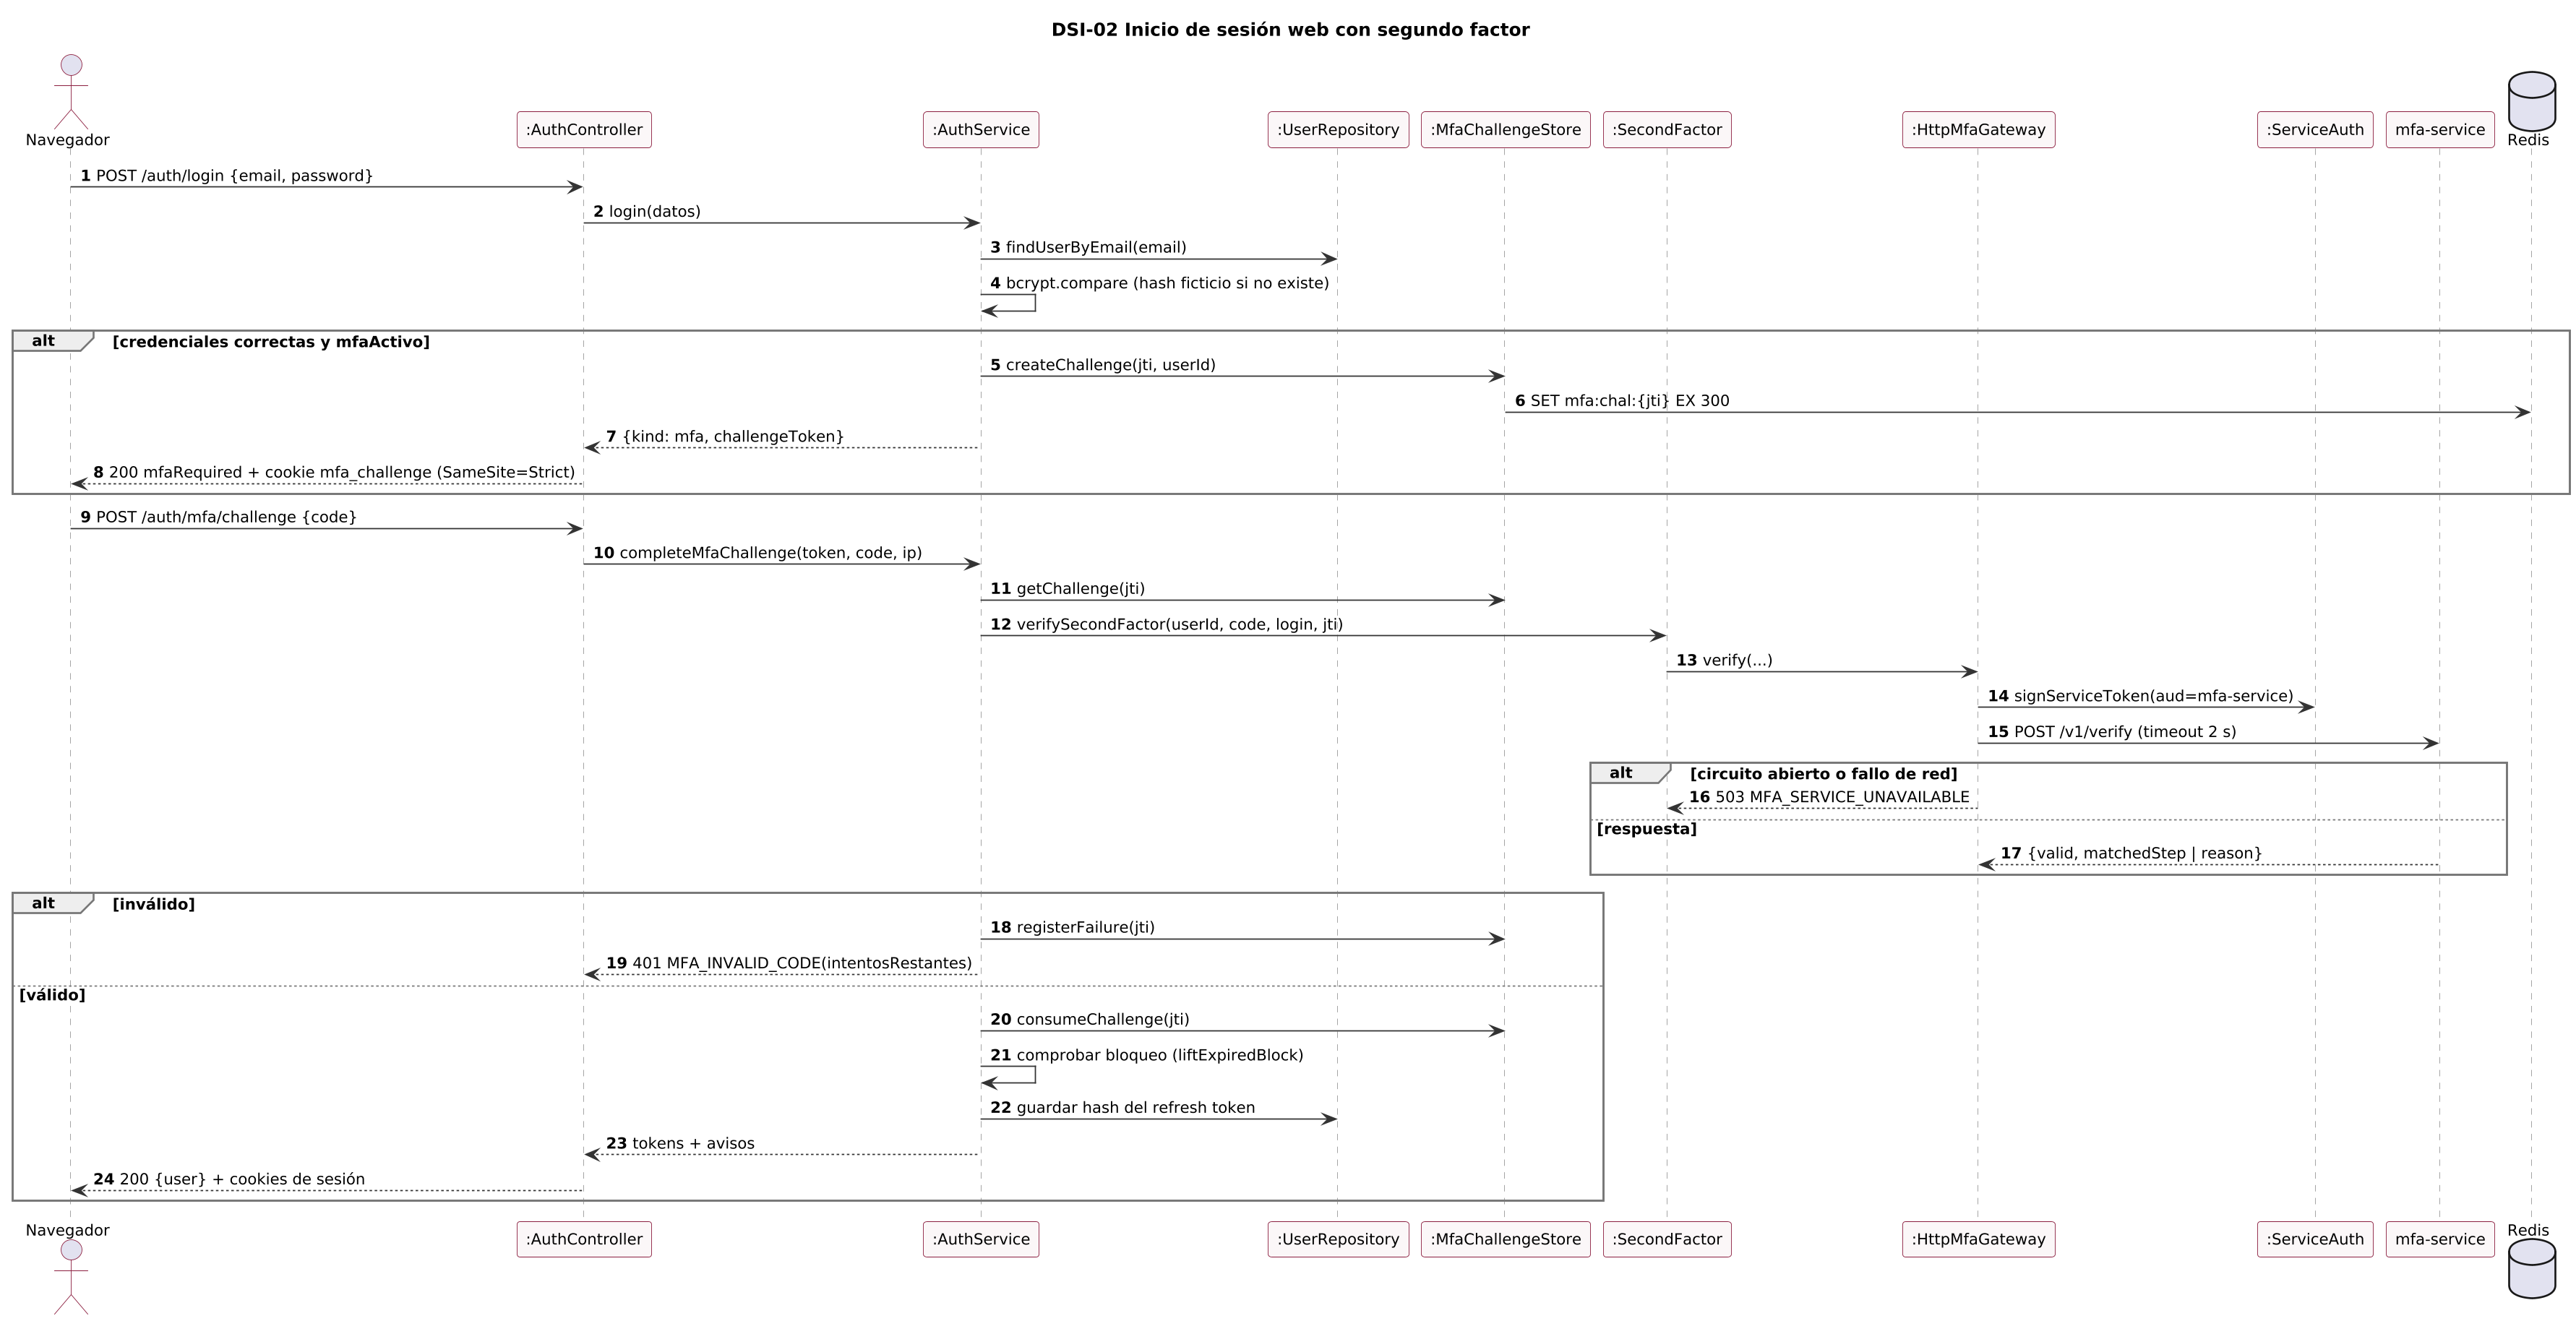
\includegraphics[width=\textheight,height=0.85\textwidth,keepaspectratio]{img/seq02-login-mfa.png}\caption{DSI-02: inicio de sesión web con segundo factor.}\label{fig:seq02-login-mfa}\end{sidewaysfigure}
\begin{sidewaysfigure}\centering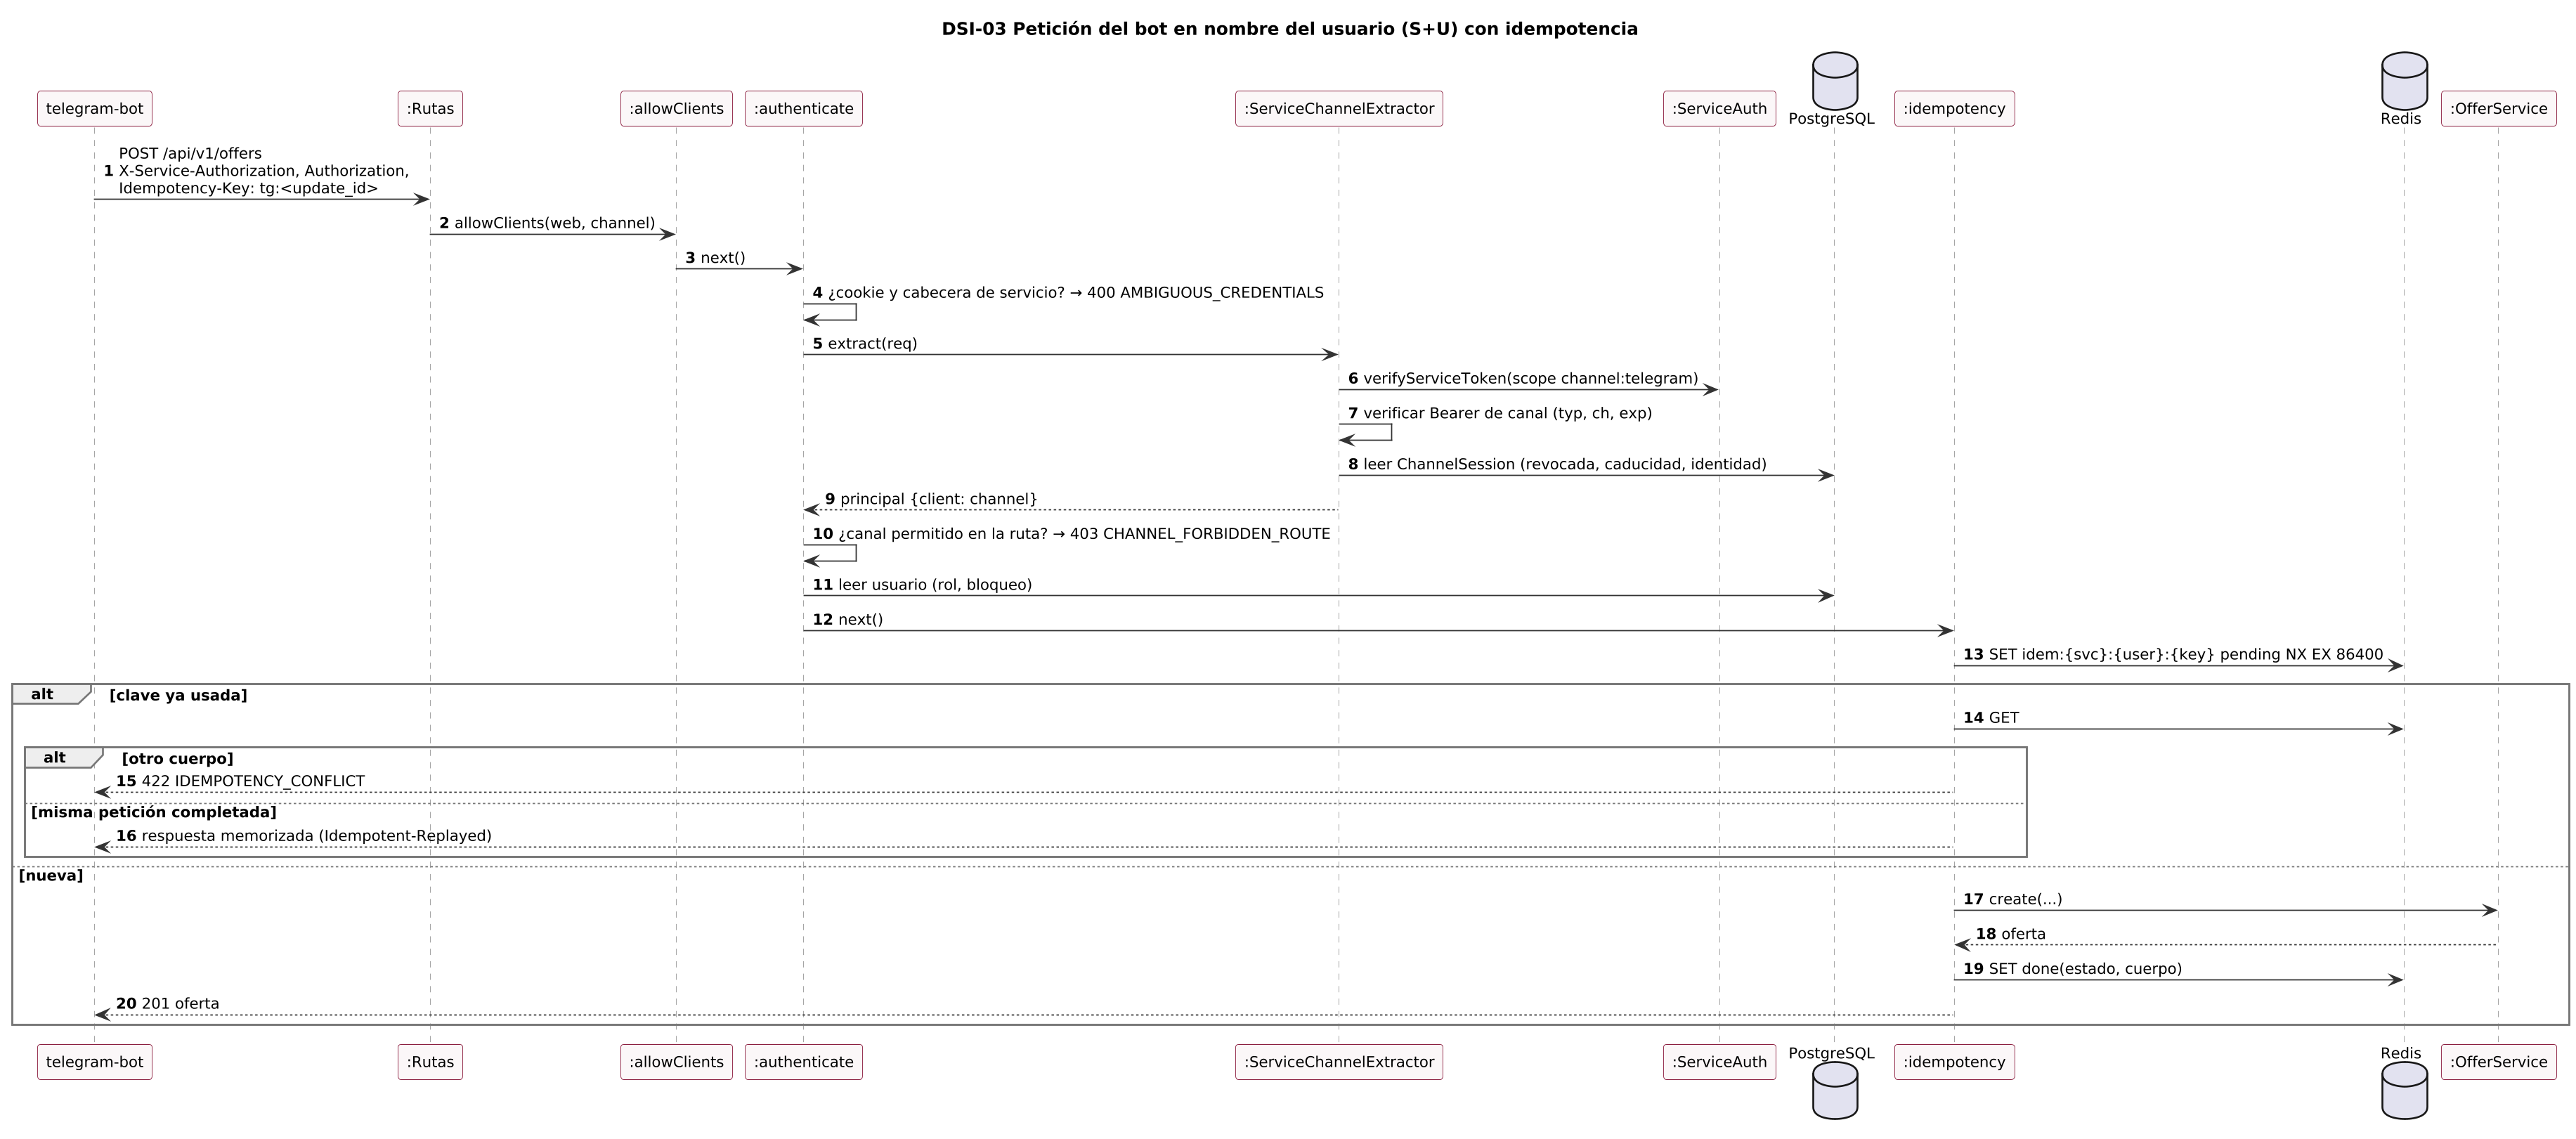
\includegraphics[width=\textheight,height=0.85\textwidth,keepaspectratio]{img/seq03-peticion-bot.png}\caption{DSI-03: petición del bot en nombre del usuario, con política de canal e idempotencia.}\label{fig:seq03-peticion-bot}\end{sidewaysfigure}
\begin{sidewaysfigure}\centering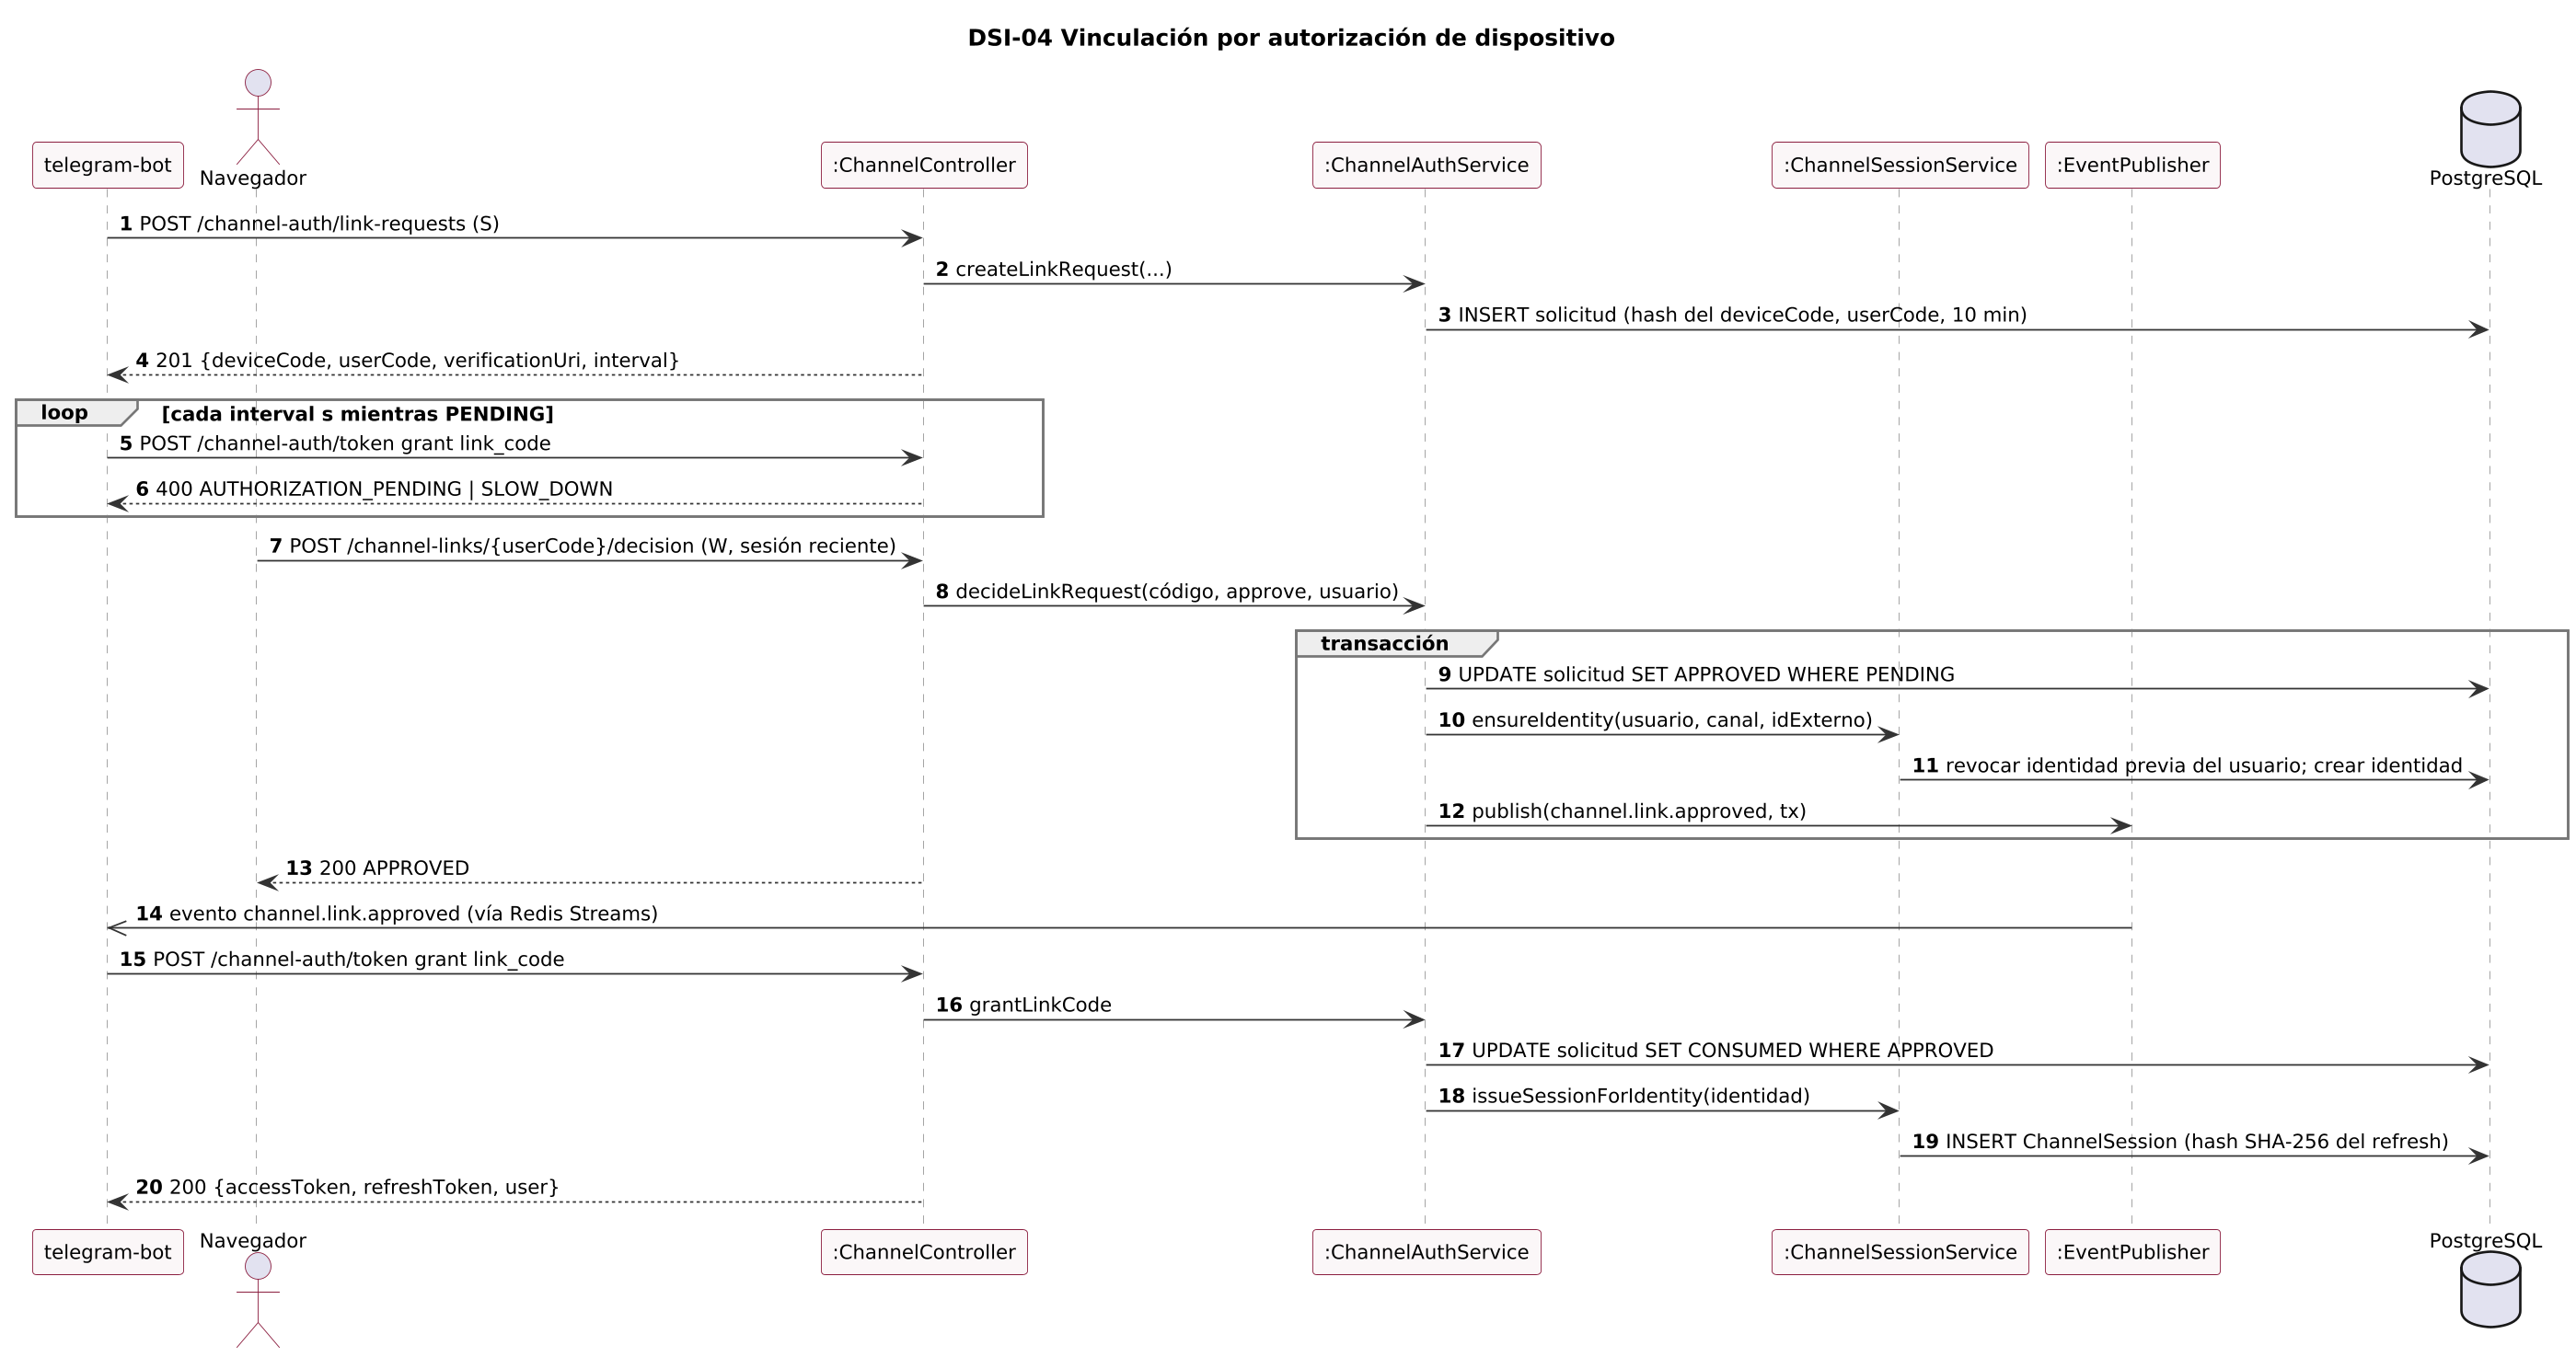
\includegraphics[width=\textheight,height=0.85\textwidth,keepaspectratio]{img/seq04-vinculacion.png}\caption{DSI-04: vinculación por autorización de dispositivo.}\label{fig:seq04-vinculacion}\end{sidewaysfigure}
\begin{figure}[H]\centering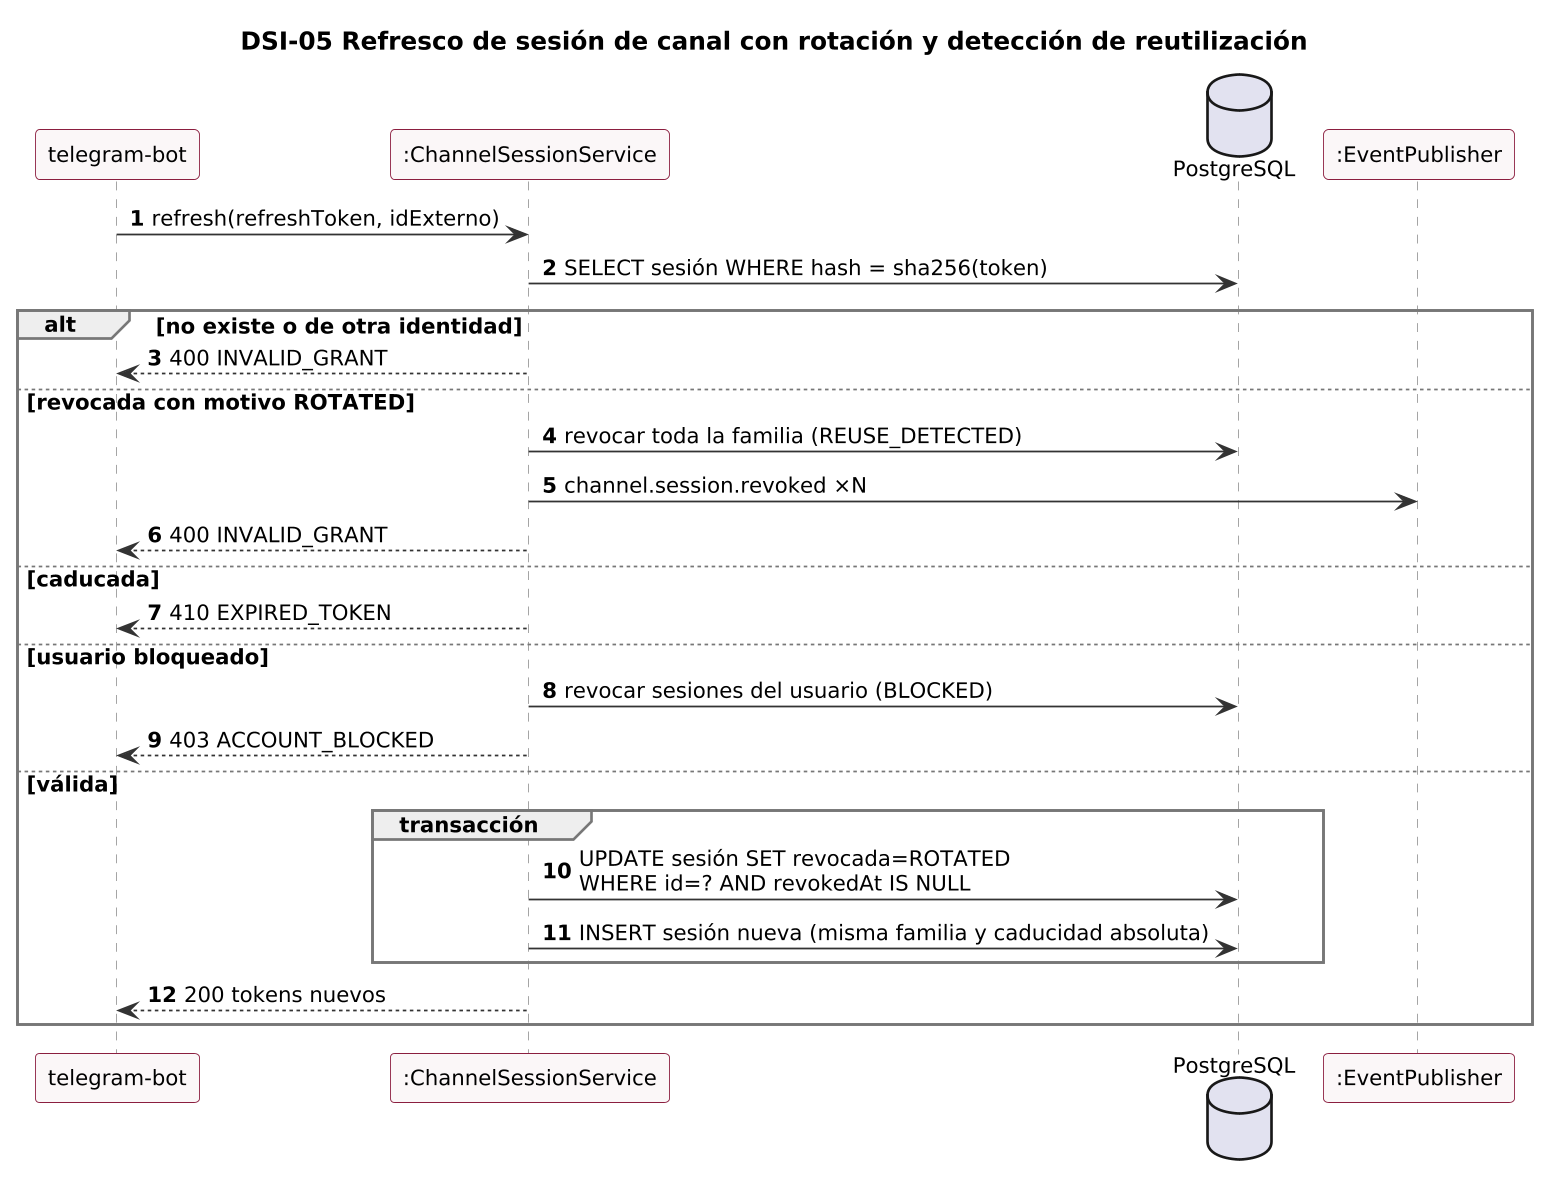
\includegraphics[width=0.85\linewidth,height=0.80\textheight,keepaspectratio]{img/seq05-refresco-canal.png}\caption{DSI-05: refresco de sesión de canal con rotación y detección de reutilización.}\label{fig:seq05-refresco-canal}\end{figure}
\begin{sidewaysfigure}\centering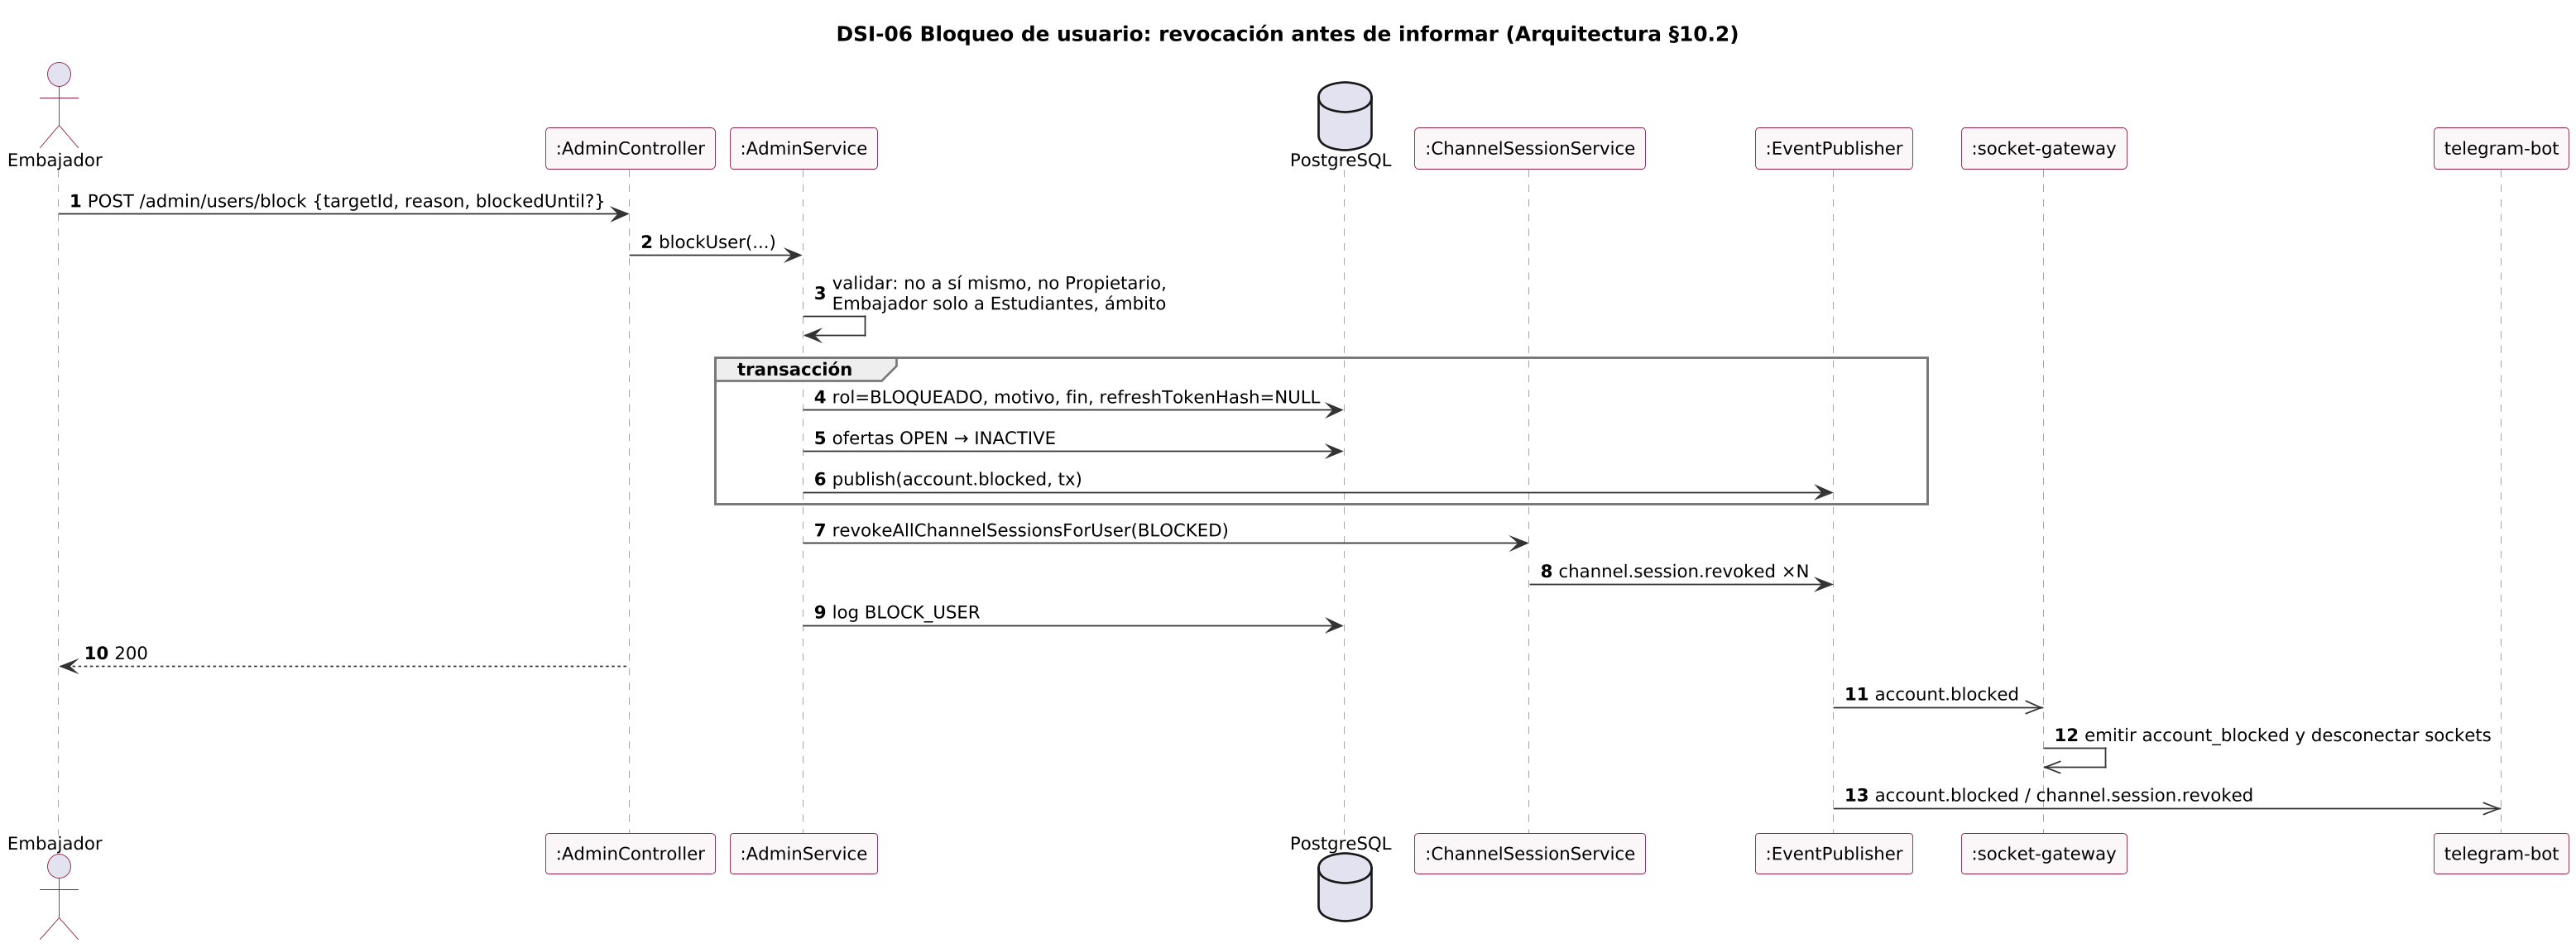
\includegraphics[width=\textheight,height=0.85\textwidth,keepaspectratio]{img/seq06-bloqueo.png}\caption{DSI-06: bloqueo de usuario, con la revocación antes del aviso.}\label{fig:seq06-bloqueo}\end{sidewaysfigure}

%════════════════════════════════════════════════════════════════════
\chapter{Especificación completa de la API}\label{cap:api}

\section{Convenciones comunes}
\begin{itemize}[leftmargin=*,itemsep=1pt]
\item \textbf{Base.} Todas las rutas cuelgan de \texttt{/api/v1}; \texttt{/api} es un alias para el frontend actual. \texttt{Content-Type: application/json}; cuerpo máximo 50~KB.
\item \textbf{Acceso.} P: público. W: sesión web por cookie. S: credencial de servicio en \texttt{X-Service-Authorization: Bearer}. S+U: servicio más \texttt{Authorization: Bearer} con token de canal. Adm: Embajador o Propietario, con comprobación de ámbito cuando se indica. Prop: solo Propietario. I: admite \texttt{Idempotency-Key} (UUID o \texttt{tg:<update\_id>}), obligatoria para clientes de canal.
\item \textbf{Política de canal.} Una ruta solo admite clientes de canal si su acceso incluye S+U; si no, responde 403 \texttt{CHANNEL\_FORBIDDEN\_ROUTE}. Enviar cookie y cabecera de servicio a la vez da 400 \texttt{AMBIGUOUS\_CREDENTIALS}.
\item \textbf{Identificadores.} Los \texttt{*Id} son CUID y se validan antes de usarse.
\item \textbf{Paginación.} Cursor opaco por \texttt{(createdAt, id)} descendente.
\item \textbf{Trazabilidad.} \texttt{X-Request-Id} se devuelve siempre y se propaga a log y eventos.
\end{itemize}

\paragraph{Contrato de error.} Todas las respuestas de error tienen la forma:
\begin{lstlisting}[language={},basicstyle=\ttfamily\small]
{ "error": "Mensaje legible en español",
  "code": "CODIGO_ESTABLE",
  "requestId": "01JC9...",
  "details": { "retryAfter": 30, "remainingAttempts": 3 } }
\end{lstlisting}
\paragraph{Respuestas comunes.} Además de las indicadas en cada endpoint, cualquiera puede devolver: 400 \texttt{VALIDATION\_ERROR} (esquema), 401 \texttt{UNAUTHORIZED}/\texttt{TOKEN\_EXPIRED}/\texttt{INVALID\_TOKEN} (rutas autenticadas), 403 \texttt{ACCOUNT\_BLOCKED} o \texttt{FORBIDDEN}, 413 \texttt{PAYLOAD\_TOO\_LARGE}, 429 \texttt{RATE\_LIMITED} con \texttt{Retry-After}, y 500 \texttt{INTERNAL\_ERROR} sin detalles internos.

\section{Resumen de endpoints}
\begin{center}\small
\begin{longtable}{@{}lp{7.3cm}p{2.8cm}p{3.4cm}@{}}
\toprule
Método & Ruta & Acceso & Grupo \\
\midrule
\endhead
POST & \texttt{/\allowbreak{}auth/\allowbreak{}register} & P & Autenticación web\\
POST & \texttt{/\allowbreak{}auth/\allowbreak{}verify-otp} & P & Autenticación web\\
POST & \texttt{/\allowbreak{}auth/\allowbreak{}login} & P & Autenticación web\\
POST & \texttt{/\allowbreak{}auth/\allowbreak{}mfa/\allowbreak{}challenge} & P (cookie de reto) & Autenticación web\\
POST & \texttt{/\allowbreak{}auth/\allowbreak{}refresh} & P (cookie) & Autenticación web\\
POST & \texttt{/\allowbreak{}auth/\allowbreak{}forgot-password} & P & Autenticación web\\
POST & \texttt{/\allowbreak{}auth/\allowbreak{}reset-password} & P & Autenticación web\\
POST & \texttt{/\allowbreak{}auth/\allowbreak{}logout} & W & Autenticación web\\
GET & \texttt{/\allowbreak{}auth/\allowbreak{}me} & W, S+U & Autenticación web\\
PATCH & \texttt{/\allowbreak{}auth/\allowbreak{}me} & W & Autenticación web\\
PATCH & \texttt{/\allowbreak{}auth/\allowbreak{}settings/\allowbreak{}password} & W & Autenticación web\\
POST & \texttt{/\allowbreak{}auth/\allowbreak{}reauthenticate} & W & Autenticación web\\
GET & \texttt{/\allowbreak{}auth/\allowbreak{}mfa} & W, S+U & Segundo factor (MFA)\\
POST & \texttt{/\allowbreak{}auth/\allowbreak{}mfa/\allowbreak{}enrollments} & W (reautenticado) & Segundo factor (MFA)\\
POST & \texttt{/\allowbreak{}auth/\allowbreak{}mfa/\allowbreak{}enrollments/\allowbreak{}\{enrollmentId\}/\allowbreak{}confirm} & W & Segundo factor (MFA)\\
DELETE & \texttt{/\allowbreak{}auth/\allowbreak{}mfa/\allowbreak{}enrollments/\allowbreak{}\{enrollmentId\}} & W & Segundo factor (MFA)\\
POST & \texttt{/\allowbreak{}auth/\allowbreak{}mfa/\allowbreak{}disable} & W & Segundo factor (MFA)\\
POST & \texttt{/\allowbreak{}auth/\allowbreak{}mfa/\allowbreak{}recovery-codes} & W & Segundo factor (MFA)\\
GET & \texttt{/\allowbreak{}public/\allowbreak{}careers} & P & Catálogo público y perfil\\
GET & \texttt{/\allowbreak{}public/\allowbreak{}careers/\allowbreak{}\{carreraId\}/\allowbreak{}courses} & P & Catálogo público y perfil\\
GET & \texttt{/\allowbreak{}public/\allowbreak{}subjects/\allowbreak{}search} & P & Catálogo público y perfil\\
GET & \texttt{/\allowbreak{}subjects/\allowbreak{}\{asignaturaId\}/\allowbreak{}groups} & W, S+U & Catálogo público y perfil\\
GET & \texttt{/\allowbreak{}me/\allowbreak{}expediente} & W, S+U & Catálogo público y perfil\\
POST & \texttt{/\allowbreak{}me/\allowbreak{}expediente} & W, S+U · I & Catálogo público y perfil\\
DELETE & \texttt{/\allowbreak{}me/\allowbreak{}expediente/\allowbreak{}\{asignaturaId\}} & W, S+U & Catálogo público y perfil\\
GET & \texttt{/\allowbreak{}me/\allowbreak{}notification-preferences} & W, S+U & Catálogo público y perfil\\
PATCH & \texttt{/\allowbreak{}me/\allowbreak{}notification-preferences} & W, S+U & Catálogo público y perfil\\
GET & \texttt{/\allowbreak{}me/\allowbreak{}channels} & W & Catálogo público y perfil\\
DELETE & \texttt{/\allowbreak{}me/\allowbreak{}channels/\allowbreak{}\{identityId\}} & W (sesión reciente) & Catálogo público y perfil\\
GET & \texttt{/\allowbreak{}offers} & W, S+U & Ofertas y chat\\
GET & \texttt{/\allowbreak{}offers/\allowbreak{}me} & W, S+U & Ofertas y chat\\
GET & \texttt{/\allowbreak{}offers/\allowbreak{}\{id\}} & W & Ofertas y chat\\
POST & \texttt{/\allowbreak{}offers} & W, S+U · I & Ofertas y chat\\
POST & \texttt{/\allowbreak{}offers/\allowbreak{}\{id\}/\allowbreak{}accept} & W, S+U · I & Ofertas y chat\\
POST & \texttt{/\allowbreak{}offers/\allowbreak{}\{id\}/\allowbreak{}messages} & W, S+U · I & Ofertas y chat\\
PATCH & \texttt{/\allowbreak{}offers/\allowbreak{}\{id\}/\allowbreak{}close} & W, S+U & Ofertas y chat\\
POST & \texttt{/\allowbreak{}tickets} & W & Tickets de soporte\\
GET & \texttt{/\allowbreak{}tickets/\allowbreak{}me} & W & Tickets de soporte\\
GET & \texttt{/\allowbreak{}tickets/\allowbreak{}\{id\}} & W & Tickets de soporte\\
PATCH & \texttt{/\allowbreak{}tickets/\allowbreak{}\{id\}/\allowbreak{}close} & W & Tickets de soporte\\
POST & \texttt{/\allowbreak{}tickets/\allowbreak{}\{id\}/\allowbreak{}messages} & W & Tickets de soporte\\
GET & \texttt{/\allowbreak{}tickets/\allowbreak{}admin/\allowbreak{}list} & Adm & Tickets de soporte\\
GET & \texttt{/\allowbreak{}notifications} & W, S+U & Notificaciones\\
GET & \texttt{/\allowbreak{}notifications/\allowbreak{}unread-count} & W, S+U & Notificaciones\\
PATCH & \texttt{/\allowbreak{}notifications/\allowbreak{}read-all} & W, S+U & Notificaciones\\
PATCH & \texttt{/\allowbreak{}notifications/\allowbreak{}\{id\}/\allowbreak{}read} & W, S+U & Notificaciones\\
GET & \texttt{/\allowbreak{}admin/\allowbreak{}careers} & Adm & Administración\\
POST & \texttt{/\allowbreak{}admin/\allowbreak{}careers} & Prop & Administración\\
DELETE & \texttt{/\allowbreak{}admin/\allowbreak{}careers/\allowbreak{}\{id\}} & Prop & Administración\\
GET & \texttt{/\allowbreak{}admin/\allowbreak{}careers/\allowbreak{}\{carreraId\}/\allowbreak{}courses} & Adm (ámbito) & Administración\\
POST & \texttt{/\allowbreak{}admin/\allowbreak{}courses} & Adm (ámbito) & Administración\\
DELETE & \texttt{/\allowbreak{}admin/\allowbreak{}courses/\allowbreak{}\{id\}} & Adm (ámbito) & Administración\\
GET & \texttt{/\allowbreak{}admin/\allowbreak{}courses/\allowbreak{}\{cursoId\}/\allowbreak{}subjects} & Adm (ámbito) & Administración\\
POST & \texttt{/\allowbreak{}admin/\allowbreak{}subjects} & Adm (ámbito) & Administración\\
DELETE & \texttt{/\allowbreak{}admin/\allowbreak{}subjects/\allowbreak{}\{id\}} & Adm (ámbito) & Administración\\
GET & \texttt{/\allowbreak{}admin/\allowbreak{}subjects/\allowbreak{}\{asignaturaId\}/\allowbreak{}groups} & Adm (ámbito) & Administración\\
POST & \texttt{/\allowbreak{}admin/\allowbreak{}groups} & Adm (ámbito) & Administración\\
DELETE & \texttt{/\allowbreak{}admin/\allowbreak{}groups/\allowbreak{}\{id\}} & Adm (ámbito) & Administración\\
GET & \texttt{/\allowbreak{}admin/\allowbreak{}users/\allowbreak{}search} & Adm & Administración\\
GET & \texttt{/\allowbreak{}admin/\allowbreak{}users/\allowbreak{}\{userId\}/\allowbreak{}details} & Adm (ámbito) & Administración\\
GET & \texttt{/\allowbreak{}admin/\allowbreak{}users/\allowbreak{}\{userId\}/\allowbreak{}logs} & Adm (ámbito) & Administración\\
POST & \texttt{/\allowbreak{}admin/\allowbreak{}users/\allowbreak{}block} & Adm (ámbito) & Administración\\
PATCH & \texttt{/\allowbreak{}admin/\allowbreak{}users/\allowbreak{}\{id\}/\allowbreak{}unblock} & Adm & Administración\\
PATCH & \texttt{/\allowbreak{}admin/\allowbreak{}users/\allowbreak{}\{userId\}/\allowbreak{}password} & Adm (ámbito) & Administración\\
POST & \texttt{/\allowbreak{}admin/\allowbreak{}users/\allowbreak{}\{id\}/\allowbreak{}mfa/\allowbreak{}reset} & Adm (ámbito) & Administración\\
GET & \texttt{/\allowbreak{}admin/\allowbreak{}ambassadors} & Prop & Administración\\
POST & \texttt{/\allowbreak{}admin/\allowbreak{}ambassadors} & Prop & Administración\\
DELETE & \texttt{/\allowbreak{}admin/\allowbreak{}ambassadors/\allowbreak{}\{id\}} & Prop & Administración\\
PATCH & \texttt{/\allowbreak{}admin/\allowbreak{}ambassadors/\allowbreak{}scope} & Prop & Administración\\
GET & \texttt{/\allowbreak{}admin/\allowbreak{}logs} & Adm & Administración\\
POST & \texttt{/\allowbreak{}service-auth/\allowbreak{}token} & Interno & Canales externos y servicios\\
GET & \texttt{/\allowbreak{}internal/\allowbreak{}.well-known/\allowbreak{}jwks.json} & Interno & Canales externos y servicios\\
POST & \texttt{/\allowbreak{}channel-auth/\allowbreak{}link-requests} & S & Canales externos y servicios\\
GET & \texttt{/\allowbreak{}channel-links/\allowbreak{}\{userCode\}} & W & Canales externos y servicios\\
POST & \texttt{/\allowbreak{}channel-links/\allowbreak{}\{userCode\}/\allowbreak{}decision} & W (sesión reciente) & Canales externos y servicios\\
POST & \texttt{/\allowbreak{}channel-auth/\allowbreak{}token} & S & Canales externos y servicios\\
POST & \texttt{/\allowbreak{}channel-auth/\allowbreak{}email-otp} & S & Canales externos y servicios\\
POST & \texttt{/\allowbreak{}channel-auth/\allowbreak{}register} & S · I & Canales externos y servicios\\
POST & \texttt{/\allowbreak{}channel-auth/\allowbreak{}revoke} & S+U & Canales externos y servicios\\
GET & \texttt{/\allowbreak{}health} & P & Canales externos y servicios\\
\bottomrule
\end{longtable}
\end{center}

\section{Detalle por endpoint}
\subsection{Autenticación web}
Rutas bajo \texttt{/\allowbreak{}auth}. El access token (15 min) y el refresh token (7 días) viajan en cookies HttpOnly; el refresh solo se envía a la ruta de renovación del prefijo usado.

\begin{apiendpoint}{\verbo{verbpost}{POST}\ \texttt{/\allowbreak{}auth/\allowbreak{}register}}{P}
\begin{tabularx}{\linewidth}{@{}>{\ttfamily\raggedright}p{3.0cm}p{1.35cm}p{1.9cm}p{0.9cm}X@{}}
\toprule \normalfont\bfseries Parámetro & \bfseries Dónde & \bfseries Tipo & \bfseries Obl. & \bfseries Descripción y validación\\ \midrule
name & cuerpo & string & Sí & 2–100 caracteres (RV-01).\\
email & cuerpo & string & Sí & Formato válido y dominio \texttt{@alumnos.unican.es} (RV-02).\\
password & cuerpo & string & Sí & $\geq$ 8; mayúscula, minúscula, número y símbolo (RV-03).\\
carreraId & cuerpo & cuid & Sí & Carrera existente y no eliminada.\\
cursoId & cuerpo & cuid & Sí & Curso de esa carrera.\\
\bottomrule\end{tabularx}
\par\smallskip\textbf{Lógica.} Crea un registro pendiente con el hash de la contraseña y del OTP, envía el OTP por correo y deja el reto en la cookie \texttt{otp\_token} (30 min). No crea la cuenta.
\par\smallskip\textbf{Respuestas.} \textbf{202} OTP enviado; \textbf{400} VALIDATION\_ERROR, INVALID\_EMAIL\_DOMAIN, WEAK\_PASSWORD; \textbf{409} EMAIL\_TAKEN; \textbf{429} RATE\_LIMITED.
\end{apiendpoint}
\begin{apiendpoint}{\verbo{verbpost}{POST}\ \texttt{/\allowbreak{}auth/\allowbreak{}verify-otp}}{P}
\begin{tabularx}{\linewidth}{@{}>{\ttfamily\raggedright}p{3.0cm}p{1.35cm}p{1.9cm}p{0.9cm}X@{}}
\toprule \normalfont\bfseries Parámetro & \bfseries Dónde & \bfseries Tipo & \bfseries Obl. & \bfseries Descripción y validación\\ \midrule
otp\_token & cookie & JWT & Sí & Reto emitido por el registro.\\
otpCode & cuerpo & string & Sí & Exactamente 6 dígitos.\\
\bottomrule\end{tabularx}
\par\smallskip\textbf{Lógica.} Comprueba el reto y el código (máximo 5 intentos), crea el usuario con rol Estudiante, borra el pendiente e inicia sesión.
\par\smallskip\textbf{Respuestas.} \textbf{201} Cuenta creada y cookies de sesión; \textbf{400} INVALID\_OTP; \textbf{401} INVALID\_TOKEN; \textbf{404} Sin registro pendiente; \textbf{410} EXPIRED\_TOKEN.
\end{apiendpoint}
\begin{apiendpoint}{\verbo{verbpost}{POST}\ \texttt{/\allowbreak{}auth/\allowbreak{}login}}{P}
\begin{tabularx}{\linewidth}{@{}>{\ttfamily\raggedright}p{3.0cm}p{1.35cm}p{1.9cm}p{0.9cm}X@{}}
\toprule \normalfont\bfseries Parámetro & \bfseries Dónde & \bfseries Tipo & \bfseries Obl. & \bfseries Descripción y validación\\ \midrule
email & cuerpo & string & Sí & Email.\\
password & cuerpo & string & Sí & Contraseña.\\
\bottomrule\end{tabularx}
\par\smallskip\textbf{Lógica.} Valida credenciales con respuesta genérica. Sin MFA: emite la sesión, registra el acceso y notifica. Con MFA: no emite sesión; devuelve \texttt{mfaRequired} y la cookie \texttt{mfa\_challenge} (5 min, SameSite=Strict, ruta del reto).
\par\smallskip\textbf{Respuestas.} \textbf{200} Sesión iniciada, o \texttt{\{mfaRequired,\allowbreak{} methods,\allowbreak{} expiresIn\}}; \textbf{401} INVALID\_CREDENTIALS; \textbf{403} ACCOUNT\_BLOCKED con \texttt{detail} (motivo, fin); \textbf{429} RATE\_LIMITED.
\end{apiendpoint}
\begin{apiendpoint}{\verbo{verbpost}{POST}\ \texttt{/\allowbreak{}auth/\allowbreak{}mfa/\allowbreak{}challenge}}{P (cookie de reto)}
\begin{tabularx}{\linewidth}{@{}>{\ttfamily\raggedright}p{3.0cm}p{1.35cm}p{1.9cm}p{0.9cm}X@{}}
\toprule \normalfont\bfseries Parámetro & \bfseries Dónde & \bfseries Tipo & \bfseries Obl. & \bfseries Descripción y validación\\ \midrule
mfa\_challenge & cookie & JWT & Sí & Reto vigente y no consumido.\\
code & cuerpo & string & Cond. & Código XOTP de 6 dígitos.\\
recoveryCode & cuerpo & string & Cond. & \texttt{XXXXX-XXXXX}; excluyente con \texttt{code}.\\
\bottomrule\end{tabularx}
\par\smallskip\textbf{Lógica.} Verifica el segundo factor contra el mfa-service (máximo 5 intentos por reto); después comprueba el bloqueo y emite la sesión. El uso de un código de recuperación se audita y se notifica.
\par\smallskip\textbf{Respuestas.} \textbf{200} \texttt{\{user,\allowbreak{} warnings?\}} y cookies de sesión; \textbf{400} VALIDATION\_ERROR; \textbf{401} MFA\_INVALID\_CODE (\texttt{remainingAttempts}, \texttt{reason}); \textbf{403} ACCOUNT\_BLOCKED; \textbf{410} MFA\_CHALLENGE\_EXPIRED; \textbf{423} MFA\_LOCKED (\texttt{retryAfter}); \textbf{503} MFA\_SERVICE\_UNAVAILABLE.
\end{apiendpoint}
\begin{apiendpoint}{\verbo{verbpost}{POST}\ \texttt{/\allowbreak{}auth/\allowbreak{}refresh}}{P (cookie)}
\begin{tabularx}{\linewidth}{@{}>{\ttfamily\raggedright}p{3.0cm}p{1.35cm}p{1.9cm}p{0.9cm}X@{}}
\toprule \normalfont\bfseries Parámetro & \bfseries Dónde & \bfseries Tipo & \bfseries Obl. & \bfseries Descripción y validación\\ \midrule
refresh\_token & cookie & JWT & Sí & Debe coincidir con el hash guardado.\\
\bottomrule\end{tabularx}
\par\smallskip\textbf{Lógica.} Emite un nuevo access token conservando el momento del login original. Si el usuario está bloqueado, revoca la sesión.
\par\smallskip\textbf{Respuestas.} \textbf{200} Token renovado; \textbf{401} INVALID\_TOKEN, SESSION\_REVOKED; \textbf{403} ACCOUNT\_BLOCKED.
\end{apiendpoint}
\begin{apiendpoint}{\verbo{verbpost}{POST}\ \texttt{/\allowbreak{}auth/\allowbreak{}forgot-password}}{P}
\begin{tabularx}{\linewidth}{@{}>{\ttfamily\raggedright}p{3.0cm}p{1.35cm}p{1.9cm}p{0.9cm}X@{}}
\toprule \normalfont\bfseries Parámetro & \bfseries Dónde & \bfseries Tipo & \bfseries Obl. & \bfseries Descripción y validación\\ \midrule
email & cuerpo & string & Sí & Email.\\
\bottomrule\end{tabularx}
\par\smallskip\textbf{Lógica.} Si existe la cuenta, sustituye cualquier solicitud anterior y envía un OTP de 15 min. La respuesta no revela la existencia.
\par\smallskip\textbf{Respuestas.} \textbf{200} Respuesta genérica; \textbf{429} RATE\_LIMITED.
\end{apiendpoint}
\begin{apiendpoint}{\verbo{verbpost}{POST}\ \texttt{/\allowbreak{}auth/\allowbreak{}reset-password}}{P}
\begin{tabularx}{\linewidth}{@{}>{\ttfamily\raggedright}p{3.0cm}p{1.35cm}p{1.9cm}p{0.9cm}X@{}}
\toprule \normalfont\bfseries Parámetro & \bfseries Dónde & \bfseries Tipo & \bfseries Obl. & \bfseries Descripción y validación\\ \midrule
email & cuerpo & string & Sí & Email.\\
otpCode & cuerpo & string & Sí & 6 dígitos.\\
newPassword & cuerpo & string & Sí & Complejidad RV-03.\\
\bottomrule\end{tabularx}
\par\smallskip\textbf{Lógica.} Fija la nueva contraseña, revoca la sesión web, consume la solicitud y registra \texttt{PASSWORD\_RESET}. No altera el MFA. Sirve para que una cuenta creada por canal fije contraseña.
\par\smallskip\textbf{Respuestas.} \textbf{200} Contraseña actualizada; \textbf{400} INVALID\_OTP, WEAK\_PASSWORD, sin solicitud; \textbf{410} EXPIRED\_TOKEN.
\end{apiendpoint}
\begin{apiendpoint}{\verbo{verbpost}{POST}\ \texttt{/\allowbreak{}auth/\allowbreak{}logout}}{W}
\textit{Sin parámetros.}
\par\smallskip\textbf{Lógica.} Anula el hash del refresh token y borra las cookies.
\par\smallskip\textbf{Respuestas.} \textbf{200} Sesión cerrada.
\end{apiendpoint}
\begin{apiendpoint}{\verbo{verbget}{GET}\ \texttt{/\allowbreak{}auth/\allowbreak{}me}}{W, S+U}
\textit{Sin parámetros.}
\par\smallskip\textbf{Lógica.} Devuelve el perfil del usuario autenticado.
\par\smallskip\textbf{Respuestas.} \textbf{200} \texttt{\{id,\allowbreak{} email,\allowbreak{} role,\allowbreak{} name,\allowbreak{} carreraId,\allowbreak{} cursoId,\allowbreak{} mfaEnabled\}}.
\end{apiendpoint}
\begin{apiendpoint}{\verbo{verbpatch}{PATCH}\ \texttt{/\allowbreak{}auth/\allowbreak{}me}}{W}
\begin{tabularx}{\linewidth}{@{}>{\ttfamily\raggedright}p{3.0cm}p{1.35cm}p{1.9cm}p{0.9cm}X@{}}
\toprule \normalfont\bfseries Parámetro & \bfseries Dónde & \bfseries Tipo & \bfseries Obl. & \bfseries Descripción y validación\\ \midrule
name & cuerpo & string & No & 2–100 caracteres.\\
carreraId & cuerpo & cuid \textbar{} null & No & Carrera.\\
cursoId & cuerpo & cuid \textbar{} null & No & Curso de la carrera.\\
\bottomrule\end{tabularx}
\par\smallskip\textbf{Lógica.} Actualiza el perfil. Cualquier otro campo (por ejemplo \texttt{email}) se rechaza (RF-PER-01).
\par\smallskip\textbf{Respuestas.} \textbf{200} Perfil actualizado; \textbf{400} Campo no permitido o curso incoherente.
\end{apiendpoint}
\begin{apiendpoint}{\verbo{verbpatch}{PATCH}\ \texttt{/\allowbreak{}auth/\allowbreak{}settings/\allowbreak{}password}}{W}
\begin{tabularx}{\linewidth}{@{}>{\ttfamily\raggedright}p{3.0cm}p{1.35cm}p{1.9cm}p{0.9cm}X@{}}
\toprule \normalfont\bfseries Parámetro & \bfseries Dónde & \bfseries Tipo & \bfseries Obl. & \bfseries Descripción y validación\\ \midrule
currentPassword & cuerpo & string & Sí & Contraseña actual.\\
newPassword & cuerpo & string & Sí & Complejidad RV-03.\\
\bottomrule\end{tabularx}
\par\smallskip\textbf{Lógica.} Cambia la contraseña tras verificar la actual.
\par\smallskip\textbf{Respuestas.} \textbf{204} Cambiada; \textbf{400} WEAK\_PASSWORD; \textbf{401} INVALID\_CREDENTIALS; \textbf{409} PASSWORD\_NOT\_SET (cuenta sin contraseña).
\end{apiendpoint}
\begin{apiendpoint}{\verbo{verbpost}{POST}\ \texttt{/\allowbreak{}auth/\allowbreak{}reauthenticate}}{W}
\begin{tabularx}{\linewidth}{@{}>{\ttfamily\raggedright}p{3.0cm}p{1.35cm}p{1.9cm}p{0.9cm}X@{}}
\toprule \normalfont\bfseries Parámetro & \bfseries Dónde & \bfseries Tipo & \bfseries Obl. & \bfseries Descripción y validación\\ \midrule
password & cuerpo & string & Cond. & Obligatoria si la cuenta tiene contraseña.\\
code & cuerpo & string & Cond. & XOTP si hay MFA; OTP de correo en el segundo paso de \texttt{email\_otp}.\\
method & cuerpo & enum & No & \texttt{password} (defecto) o \texttt{email\_otp} (cuentas sin contraseña ni MFA).\\
\bottomrule\end{tabularx}
\par\smallskip\textbf{Lógica.} Prueba de presencia reciente: rota el access token con la marca de reautenticación, válida 10 minutos.
\par\smallskip\textbf{Respuestas.} \textbf{200} Identidad verificada; \textbf{202} OTP de correo enviado (primer paso de \texttt{email\_otp}); \textbf{401} INVALID\_CREDENTIALS, MFA\_REQUIRED, MFA\_INVALID\_CODE; \textbf{423} MFA\_LOCKED; \textbf{503} MFA\_SERVICE\_UNAVAILABLE.
\end{apiendpoint}
\subsection{Segundo factor (MFA)}
El core actúa como parte confiante: el navegador nunca habla con el mfa-service. Las respuestas con secretos o códigos llevan \texttt{Cache-Control: no-store}.

\begin{apiendpoint}{\verbo{verbget}{GET}\ \texttt{/\allowbreak{}auth/\allowbreak{}mfa}}{W, S+U}
\textit{Sin parámetros.}
\par\smallskip\textbf{Lógica.} Estado del factor. Si el mfa-service no responde y el usuario no tiene MFA, responde con el estado del core marcado \texttt{degraded}.
\par\smallskip\textbf{Respuestas.} \textbf{200} \texttt{\{enabled,\allowbreak{} method,\allowbreak{} enabledAt,\allowbreak{} recoveryCodesRemaining,\allowbreak{} pendingEnrollment\}}; \textbf{503} MFA\_SERVICE\_UNAVAILABLE.
\end{apiendpoint}
\begin{apiendpoint}{\verbo{verbpost}{POST}\ \texttt{/\allowbreak{}auth/\allowbreak{}mfa/\allowbreak{}enrollments}}{W (reautenticado)}
\textit{Sin parámetros.}
\par\smallskip\textbf{Lógica.} Crea un enrolamiento pendiente (10 min) en el mfa-service y devuelve la URI XOTP firmada y los datos de introducción manual. En producción exige HTTPS.
\par\smallskip\textbf{Respuestas.} \textbf{201} \texttt{\{enrollmentId,\allowbreak{} provisioningUri,\allowbreak{} manualEntry,\allowbreak{} expiresAt\}}; \textbf{401} REAUTH\_REQUIRED; \textbf{403} HTTPS\_REQUIRED; \textbf{409} MFA\_ALREADY\_ENABLED; \textbf{503} MFA\_SERVICE\_UNAVAILABLE.
\end{apiendpoint}
\begin{apiendpoint}{\verbo{verbpost}{POST}\ \texttt{/\allowbreak{}auth/\allowbreak{}mfa/\allowbreak{}enrollments/\allowbreak{}\{enrollmentId\}/\allowbreak{}confirm}}{W}
\begin{tabularx}{\linewidth}{@{}>{\ttfamily\raggedright}p{3.0cm}p{1.35cm}p{1.9cm}p{0.9cm}X@{}}
\toprule \normalfont\bfseries Parámetro & \bfseries Dónde & \bfseries Tipo & \bfseries Obl. & \bfseries Descripción y validación\\ \midrule
enrollmentId & ruta & string & Sí & Enrolamiento propio pendiente.\\
code & cuerpo & string & Sí & Código generado por la app.\\
\bottomrule\end{tabularx}
\par\smallskip\textbf{Lógica.} Activa el factor, marca el MFA en el usuario, registra \texttt{MFA\_ENABLED}, notifica y rota las cookies de sesión. Los códigos de recuperación se devuelven una sola vez.
\par\smallskip\textbf{Respuestas.} \textbf{200} \texttt{\{enabled: true,\allowbreak{} recoveryCodes[10]\}}; \textbf{401} MFA\_INVALID\_CODE; \textbf{404} No encontrado; \textbf{409} MFA\_ALREADY\_ENABLED; \textbf{410} ENROLLMENT\_EXPIRED; \textbf{423} MFA\_LOCKED; \textbf{503} MFA\_SERVICE\_UNAVAILABLE.
\end{apiendpoint}
\begin{apiendpoint}{\verbo{verbdelete}{DELETE}\ \texttt{/\allowbreak{}auth/\allowbreak{}mfa/\allowbreak{}enrollments/\allowbreak{}\{enrollmentId\}}}{W}
\begin{tabularx}{\linewidth}{@{}>{\ttfamily\raggedright}p{3.0cm}p{1.35cm}p{1.9cm}p{0.9cm}X@{}}
\toprule \normalfont\bfseries Parámetro & \bfseries Dónde & \bfseries Tipo & \bfseries Obl. & \bfseries Descripción y validación\\ \midrule
enrollmentId & ruta & string & Sí & Enrolamiento propio pendiente.\\
\bottomrule\end{tabularx}
\par\smallskip\textbf{Lógica.} Cancela un enrolamiento pendiente.
\par\smallskip\textbf{Respuestas.} \textbf{204} Cancelado.
\end{apiendpoint}
\begin{apiendpoint}{\verbo{verbpost}{POST}\ \texttt{/\allowbreak{}auth/\allowbreak{}mfa/\allowbreak{}disable}}{W}
\begin{tabularx}{\linewidth}{@{}>{\ttfamily\raggedright}p{3.0cm}p{1.35cm}p{1.9cm}p{0.9cm}X@{}}
\toprule \normalfont\bfseries Parámetro & \bfseries Dónde & \bfseries Tipo & \bfseries Obl. & \bfseries Descripción y validación\\ \midrule
password & cuerpo & string & Cond. & Obligatoria si la cuenta tiene contraseña.\\
code & cuerpo & string & Cond. & XOTP.\\
recoveryCode & cuerpo & string & Cond. & Excluyente con \texttt{code}.\\
\bottomrule\end{tabularx}
\par\smallskip\textbf{Lógica.} Verifica contraseña y factor, borra el factor en el mfa-service, desactiva el MFA, registra \texttt{MFA\_DISABLED} y notifica.
\par\smallskip\textbf{Respuestas.} \textbf{204} Desactivado; \textbf{400} Falta el factor; \textbf{401} INVALID\_CREDENTIALS, MFA\_INVALID\_CODE; \textbf{409} MFA\_NOT\_ENABLED; \textbf{423} MFA\_LOCKED; \textbf{503} MFA\_SERVICE\_UNAVAILABLE.
\end{apiendpoint}
\begin{apiendpoint}{\verbo{verbpost}{POST}\ \texttt{/\allowbreak{}auth/\allowbreak{}mfa/\allowbreak{}recovery-codes}}{W}
\begin{tabularx}{\linewidth}{@{}>{\ttfamily\raggedright}p{3.0cm}p{1.35cm}p{1.9cm}p{0.9cm}X@{}}
\toprule \normalfont\bfseries Parámetro & \bfseries Dónde & \bfseries Tipo & \bfseries Obl. & \bfseries Descripción y validación\\ \midrule
code & cuerpo & string & Sí & XOTP válido.\\
\bottomrule\end{tabularx}
\par\smallskip\textbf{Lógica.} Regenera los 10 códigos de recuperación y anula los anteriores; registra \texttt{MFA\_RECOVERY\_REGENERATED}.
\par\smallskip\textbf{Respuestas.} \textbf{200} \texttt{\{recoveryCodes[10]\}}; \textbf{401} MFA\_INVALID\_CODE; \textbf{409} MFA\_NOT\_ENABLED; \textbf{423} MFA\_LOCKED; \textbf{503} MFA\_SERVICE\_UNAVAILABLE.
\end{apiendpoint}
\subsection{Catálogo público y perfil}
Lecturas sin sesión para el registro y recursos del propio usuario bajo \texttt{/\allowbreak{}me}.

\begin{apiendpoint}{\verbo{verbget}{GET}\ \texttt{/\allowbreak{}public/\allowbreak{}careers}}{P}
\textit{Sin parámetros.}
\par\smallskip\textbf{Lógica.} Carreras no eliminadas.
\par\smallskip\textbf{Respuestas.} \textbf{200} Lista de carreras.
\end{apiendpoint}
\begin{apiendpoint}{\verbo{verbget}{GET}\ \texttt{/\allowbreak{}public/\allowbreak{}careers/\allowbreak{}\{carreraId\}/\allowbreak{}courses}}{P}
\begin{tabularx}{\linewidth}{@{}>{\ttfamily\raggedright}p{3.0cm}p{1.35cm}p{1.9cm}p{0.9cm}X@{}}
\toprule \normalfont\bfseries Parámetro & \bfseries Dónde & \bfseries Tipo & \bfseries Obl. & \bfseries Descripción y validación\\ \midrule
carreraId & ruta & cuid & Sí & Carrera.\\
\bottomrule\end{tabularx}
\par\smallskip\textbf{Lógica.} Cursos no eliminados de la carrera.
\par\smallskip\textbf{Respuestas.} \textbf{200} Lista de cursos.
\end{apiendpoint}
\begin{apiendpoint}{\verbo{verbget}{GET}\ \texttt{/\allowbreak{}public/\allowbreak{}subjects/\allowbreak{}search}}{P}
\begin{tabularx}{\linewidth}{@{}>{\ttfamily\raggedright}p{3.0cm}p{1.35cm}p{1.9cm}p{0.9cm}X@{}}
\toprule \normalfont\bfseries Parámetro & \bfseries Dónde & \bfseries Tipo & \bfseries Obl. & \bfseries Descripción y validación\\ \midrule
q & consulta & string & No & Texto en código o nombre; máximo 100 caracteres.\\
\bottomrule\end{tabularx}
\par\smallskip\textbf{Lógica.} Asignaturas activas (sin ancestro eliminado), con sus grupos y su curso; máximo 20.
\par\smallskip\textbf{Respuestas.} \textbf{200} Lista de asignaturas.
\end{apiendpoint}
\begin{apiendpoint}{\verbo{verbget}{GET}\ \texttt{/\allowbreak{}subjects/\allowbreak{}\{asignaturaId\}/\allowbreak{}groups}}{W, S+U}
\begin{tabularx}{\linewidth}{@{}>{\ttfamily\raggedright}p{3.0cm}p{1.35cm}p{1.9cm}p{0.9cm}X@{}}
\toprule \normalfont\bfseries Parámetro & \bfseries Dónde & \bfseries Tipo & \bfseries Obl. & \bfseries Descripción y validación\\ \midrule
asignaturaId & ruta & cuid & Sí & Asignatura activa.\\
\bottomrule\end{tabularx}
\par\smallskip\textbf{Lógica.} Grupos de la asignatura ordenados por nombre, sin pasar por la administración (EP-C-14).
\par\smallskip\textbf{Respuestas.} \textbf{200} \texttt{[\{id,\allowbreak{} nombre\}]}; \textbf{400} Identificador inválido; \textbf{404} NOT\_FOUND.
\end{apiendpoint}
\begin{apiendpoint}{\verbo{verbget}{GET}\ \texttt{/\allowbreak{}me/\allowbreak{}expediente}}{W, S+U}
\textit{Sin parámetros.}
\par\smallskip\textbf{Lógica.} Asignaturas activas del expediente con grupos y curso.
\par\smallskip\textbf{Respuestas.} \textbf{200} Lista de asignaturas.
\end{apiendpoint}
\begin{apiendpoint}{\verbo{verbpost}{POST}\ \texttt{/\allowbreak{}me/\allowbreak{}expediente}}{W, S+U · I}
\begin{tabularx}{\linewidth}{@{}>{\ttfamily\raggedright}p{3.0cm}p{1.35cm}p{1.9cm}p{0.9cm}X@{}}
\toprule \normalfont\bfseries Parámetro & \bfseries Dónde & \bfseries Tipo & \bfseries Obl. & \bfseries Descripción y validación\\ \midrule
asignaturaId & cuerpo & cuid & Sí & Asignatura activa.\\
\bottomrule\end{tabularx}
\par\smallskip\textbf{Lógica.} Añade la asignatura al expediente; si ya estaba, no cambia nada.
\par\smallskip\textbf{Respuestas.} \textbf{201} Añadida; \textbf{200} Ya estaba; \textbf{404} Asignatura inexistente; \textbf{422} IDEMPOTENCY\_CONFLICT.
\end{apiendpoint}
\begin{apiendpoint}{\verbo{verbdelete}{DELETE}\ \texttt{/\allowbreak{}me/\allowbreak{}expediente/\allowbreak{}\{asignaturaId\}}}{W, S+U}
\begin{tabularx}{\linewidth}{@{}>{\ttfamily\raggedright}p{3.0cm}p{1.35cm}p{1.9cm}p{0.9cm}X@{}}
\toprule \normalfont\bfseries Parámetro & \bfseries Dónde & \bfseries Tipo & \bfseries Obl. & \bfseries Descripción y validación\\ \midrule
asignaturaId & ruta & cuid & Sí & Asignatura.\\
\bottomrule\end{tabularx}
\par\smallskip\textbf{Lógica.} Quita la asignatura del expediente.
\par\smallskip\textbf{Respuestas.} \textbf{200} Eliminada; \textbf{400} Identificador inválido.
\end{apiendpoint}
\begin{apiendpoint}{\verbo{verbget}{GET}\ \texttt{/\allowbreak{}me/\allowbreak{}notification-preferences}}{W, S+U}
\textit{Sin parámetros.}
\par\smallskip\textbf{Lógica.} Preferencias por canal.
\par\smallskip\textbf{Respuestas.} \textbf{200} \texttt{\{email: \{enabled,\allowbreak{} editable: false\},\allowbreak{} telegram: \{enabled,\allowbreak{} linked,\allowbreak{} chatMessages\},\allowbreak{} web: \{enabled\}\}}.
\end{apiendpoint}
\begin{apiendpoint}{\verbo{verbpatch}{PATCH}\ \texttt{/\allowbreak{}me/\allowbreak{}notification-preferences}}{W, S+U}
\begin{tabularx}{\linewidth}{@{}>{\ttfamily\raggedright}p{3.0cm}p{1.35cm}p{1.9cm}p{0.9cm}X@{}}
\toprule \normalfont\bfseries Parámetro & \bfseries Dónde & \bfseries Tipo & \bfseries Obl. & \bfseries Descripción y validación\\ \midrule
email.enabled & cuerpo & boolean & No & Solo se admite \texttt{true}.\\
telegram.enabled & cuerpo & boolean & No & Activa o silencia la entrega por Telegram.\\
telegram.chatMessages & cuerpo & boolean & No & Si es \texttt{false}, no se retransmite cada mensaje de chat.\\
\bottomrule\end{tabularx}
\par\smallskip\textbf{Lógica.} Actualiza las preferencias; Telegram requiere identidad vinculada.
\par\smallskip\textbf{Respuestas.} \textbf{200} Preferencias resultantes; \textbf{400} EMAIL\_CHANNEL\_REQUIRED; \textbf{409} CHANNEL\_NOT\_LINKED.
\end{apiendpoint}
\begin{apiendpoint}{\verbo{verbget}{GET}\ \texttt{/\allowbreak{}me/\allowbreak{}channels}}{W}
\textit{Sin parámetros.}
\par\smallskip\textbf{Lógica.} Identidades de canal activas del usuario.
\par\smallskip\textbf{Respuestas.} \textbf{200} \texttt{[\{identityId,\allowbreak{} channel,\allowbreak{} displayName,\allowbreak{} linkedAt,\allowbreak{} lastUsedAt\}]}.
\end{apiendpoint}
\begin{apiendpoint}{\verbo{verbdelete}{DELETE}\ \texttt{/\allowbreak{}me/\allowbreak{}channels/\allowbreak{}\{identityId\}}}{W (sesión reciente)}
\begin{tabularx}{\linewidth}{@{}>{\ttfamily\raggedright}p{3.0cm}p{1.35cm}p{1.9cm}p{0.9cm}X@{}}
\toprule \normalfont\bfseries Parámetro & \bfseries Dónde & \bfseries Tipo & \bfseries Obl. & \bfseries Descripción y validación\\ \midrule
identityId & ruta & cuid & Sí & Identidad propia.\\
\bottomrule\end{tabularx}
\par\smallskip\textbf{Lógica.} Revoca la identidad y sus sesiones; publica \texttt{channel.session.revoked} y registra \texttt{CHANNEL\_UNLINKED}.
\par\smallskip\textbf{Respuestas.} \textbf{204} Desvinculada; \textbf{401} REAUTH\_REQUIRED; \textbf{404} NOT\_FOUND.
\end{apiendpoint}
\subsection{Ofertas y chat}
Sin \texttt{limit} ni canal, los listados conservan el formato de array de la web; con \texttt{limit} (o desde un canal) devuelven \texttt{\{items,\allowbreak{} nextCursor\}}.

\begin{apiendpoint}{\verbo{verbget}{GET}\ \texttt{/\allowbreak{}offers}}{W, S+U}
\begin{tabularx}{\linewidth}{@{}>{\ttfamily\raggedright}p{3.0cm}p{1.35cm}p{1.9cm}p{0.9cm}X@{}}
\toprule \normalfont\bfseries Parámetro & \bfseries Dónde & \bfseries Tipo & \bfseries Obl. & \bfseries Descripción y validación\\ \midrule
asignaturaId & consulta & cuid & No & Asignatura de la búsqueda.\\
grupoActualId & consulta & cuid & No & Grupo que tiene el buscador.\\
grupoDeseadoId & consulta & cuid & No & Grupo que quiere; distinto del actual.\\
limit & consulta & entero & No & 1–50; 10 por defecto para canal.\\
cursor & consulta & string & No & Opaco, devuelto como \texttt{nextCursor}.\\
\bottomrule\end{tabularx}
\par\smallskip\textbf{Lógica.} Ofertas OPEN complementarias, sin entidades eliminadas, de más reciente a más antigua (RF-OFE-04, 05). En modo paginado excluye las propias y no expone el email del creador.
\par\smallskip\textbf{Respuestas.} \textbf{200} Array, o \texttt{\{items,\allowbreak{} nextCursor\}}; \textbf{400} Parámetros o cursor inválidos.
\end{apiendpoint}
\begin{apiendpoint}{\verbo{verbget}{GET}\ \texttt{/\allowbreak{}offers/\allowbreak{}me}}{W, S+U}
\begin{tabularx}{\linewidth}{@{}>{\ttfamily\raggedright}p{3.0cm}p{1.35cm}p{1.9cm}p{0.9cm}X@{}}
\toprule \normalfont\bfseries Parámetro & \bfseries Dónde & \bfseries Tipo & \bfseries Obl. & \bfseries Descripción y validación\\ \midrule
status & consulta & lista de enum & No & OPEN, ACCEPTED, CLOSED, INACTIVE separados por comas.\\
role & consulta & enum & No & \texttt{creator}, \texttt{acceptor} o \texttt{any}.\\
limit & consulta & entero & No & 1–50.\\
cursor & consulta & string & No & Opaco.\\
\bottomrule\end{tabularx}
\par\smallskip\textbf{Lógica.} Ofertas creadas o aceptadas por el usuario. En modo paginado incluye \texttt{isCreator} y la contraparte solo si la oferta está ACCEPTED.
\par\smallskip\textbf{Respuestas.} \textbf{200} Array, o \texttt{\{items,\allowbreak{} nextCursor\}}; \textbf{400} Parámetros inválidos.
\end{apiendpoint}
\begin{apiendpoint}{\verbo{verbget}{GET}\ \texttt{/\allowbreak{}offers/\allowbreak{}\{id\}}}{W}
\begin{tabularx}{\linewidth}{@{}>{\ttfamily\raggedright}p{3.0cm}p{1.35cm}p{1.9cm}p{0.9cm}X@{}}
\toprule \normalfont\bfseries Parámetro & \bfseries Dónde & \bfseries Tipo & \bfseries Obl. & \bfseries Descripción y validación\\ \midrule
id & ruta & cuid & Sí & Oferta.\\
\bottomrule\end{tabularx}
\par\smallskip\textbf{Lógica.} Detalle con el historial de mensajes en orden cronológico; solo para creador y aceptante.
\par\smallskip\textbf{Respuestas.} \textbf{200} Oferta con mensajes; \textbf{403} No es parte; \textbf{404} No encontrada.
\end{apiendpoint}
\begin{apiendpoint}{\verbo{verbpost}{POST}\ \texttt{/\allowbreak{}offers}}{W, S+U · I}
\begin{tabularx}{\linewidth}{@{}>{\ttfamily\raggedright}p{3.0cm}p{1.35cm}p{1.9cm}p{0.9cm}X@{}}
\toprule \normalfont\bfseries Parámetro & \bfseries Dónde & \bfseries Tipo & \bfseries Obl. & \bfseries Descripción y validación\\ \midrule
asignaturaId & cuerpo & cuid & Sí & Asignatura activa.\\
grupoActualId & cuerpo & cuid & Sí & Grupo de esa asignatura.\\
grupoDeseadoId & cuerpo & cuid & Sí & Grupo de esa asignatura, distinto del actual.\\
\bottomrule\end{tabularx}
\par\smallskip\textbf{Lógica.} Publica la oferta OPEN, registra \texttt{CREATE\_OFFER} y notifica al creador (RF-OFE-07). Exige expediente no vacío.
\par\smallskip\textbf{Respuestas.} \textbf{201} Oferta creada; \textbf{400} Grupos inválidos o iguales; \textbf{403} ACCOUNT\_BLOCKED; \textbf{409} EXPEDIENTE\_REQUIRED; \textbf{422} IDEMPOTENCY\_CONFLICT.
\end{apiendpoint}
\begin{apiendpoint}{\verbo{verbpost}{POST}\ \texttt{/\allowbreak{}offers/\allowbreak{}\{id\}/\allowbreak{}accept}}{W, S+U · I}
\begin{tabularx}{\linewidth}{@{}>{\ttfamily\raggedright}p{3.0cm}p{1.35cm}p{1.9cm}p{0.9cm}X@{}}
\toprule \normalfont\bfseries Parámetro & \bfseries Dónde & \bfseries Tipo & \bfseries Obl. & \bfseries Descripción y validación\\ \midrule
id & ruta & cuid & Sí & Oferta OPEN de otro usuario.\\
\bottomrule\end{tabularx}
\par\smallskip\textbf{Lógica.} Transición atómica OPEN $\rightarrow$ ACCEPTED mediante actualización condicional; publica \texttt{offer.status.changed} en la misma transacción y notifica a ambas partes con los datos de la contraparte.
\par\smallskip\textbf{Respuestas.} \textbf{200} Oferta aceptada; \textbf{400} OWN\_OFFER; \textbf{403} ACCOUNT\_BLOCKED; \textbf{404} No encontrada; \textbf{409} OFFER\_NOT\_OPEN, EXPEDIENTE\_REQUIRED.
\end{apiendpoint}
\begin{apiendpoint}{\verbo{verbpost}{POST}\ \texttt{/\allowbreak{}offers/\allowbreak{}\{id\}/\allowbreak{}messages}}{W, S+U · I}
\begin{tabularx}{\linewidth}{@{}>{\ttfamily\raggedright}p{3.0cm}p{1.35cm}p{1.9cm}p{0.9cm}X@{}}
\toprule \normalfont\bfseries Parámetro & \bfseries Dónde & \bfseries Tipo & \bfseries Obl. & \bfseries Descripción y validación\\ \midrule
id & ruta & cuid & Sí & Oferta ACCEPTED de la que el usuario es parte.\\
content & cuerpo & string & Sí & 1–2000 caracteres tras recortar espacios.\\
\bottomrule\end{tabularx}
\par\smallskip\textbf{Lógica.} Revalida pertenencia y estado, persiste el mensaje antes de difundirlo (\texttt{offer.message.created}) y notifica a ambas partes.
\par\smallskip\textbf{Respuestas.} \textbf{201} \texttt{\{id,\allowbreak{} content,\allowbreak{} timestamp,\allowbreak{} authorId,\allowbreak{} author\}}; \textbf{400} Longitud inválida; \textbf{403} No es parte; \textbf{404} No encontrada; \textbf{409} CHAT\_CLOSED.
\end{apiendpoint}
\begin{apiendpoint}{\verbo{verbpatch}{PATCH}\ \texttt{/\allowbreak{}offers/\allowbreak{}\{id\}/\allowbreak{}close}}{W, S+U}
\begin{tabularx}{\linewidth}{@{}>{\ttfamily\raggedright}p{3.0cm}p{1.35cm}p{1.9cm}p{0.9cm}X@{}}
\toprule \normalfont\bfseries Parámetro & \bfseries Dónde & \bfseries Tipo & \bfseries Obl. & \bfseries Descripción y validación\\ \midrule
id & ruta & cuid & Sí & Oferta del creador o del aceptante; o cualquiera para administradores.\\
\bottomrule\end{tabularx}
\par\smallskip\textbf{Lógica.} Cierre condicional; publica \texttt{offer.status.changed} y registra \texttt{CLOSE\_OFFER}. Un estado CLOSED es final.
\par\smallskip\textbf{Respuestas.} \textbf{200} Oferta cerrada; \textbf{403} Sin permiso; \textbf{404} No encontrada; \textbf{409} OFFER\_ALREADY\_CLOSED.
\end{apiendpoint}
\subsection{Tickets de soporte}
Solo interfaz web.

\begin{apiendpoint}{\verbo{verbpost}{POST}\ \texttt{/\allowbreak{}tickets}}{W}
\begin{tabularx}{\linewidth}{@{}>{\ttfamily\raggedright}p{3.0cm}p{1.35cm}p{1.9cm}p{0.9cm}X@{}}
\toprule \normalfont\bfseries Parámetro & \bfseries Dónde & \bfseries Tipo & \bfseries Obl. & \bfseries Descripción y validación\\ \midrule
asunto & cuerpo & string & Sí & 3–200 caracteres.\\
mensaje & cuerpo & string & No & Mensaje inicial, 1–2000 caracteres.\\
\bottomrule\end{tabularx}
\par\smallskip\textbf{Lógica.} Abre un ticket OPEN y registra \texttt{OPEN\_TICKET}.
\par\smallskip\textbf{Respuestas.} \textbf{201} Ticket creado; \textbf{400} Validación.
\end{apiendpoint}
\begin{apiendpoint}{\verbo{verbget}{GET}\ \texttt{/\allowbreak{}tickets/\allowbreak{}me}}{W}
\textit{Sin parámetros.}
\par\smallskip\textbf{Lógica.} Tickets propios, abiertos y cerrados.
\par\smallskip\textbf{Respuestas.} \textbf{200} Lista.
\end{apiendpoint}
\begin{apiendpoint}{\verbo{verbget}{GET}\ \texttt{/\allowbreak{}tickets/\allowbreak{}\{id\}}}{W}
\begin{tabularx}{\linewidth}{@{}>{\ttfamily\raggedright}p{3.0cm}p{1.35cm}p{1.9cm}p{0.9cm}X@{}}
\toprule \normalfont\bfseries Parámetro & \bfseries Dónde & \bfseries Tipo & \bfseries Obl. & \bfseries Descripción y validación\\ \midrule
id & ruta & cuid & Sí & Ticket.\\
\bottomrule\end{tabularx}
\par\smallskip\textbf{Lógica.} Detalle y mensajes; para el creador o administradores.
\par\smallskip\textbf{Respuestas.} \textbf{200} Ticket; \textbf{403} Sin acceso; \textbf{404} No encontrado.
\end{apiendpoint}
\begin{apiendpoint}{\verbo{verbpatch}{PATCH}\ \texttt{/\allowbreak{}tickets/\allowbreak{}\{id\}/\allowbreak{}close}}{W}
\begin{tabularx}{\linewidth}{@{}>{\ttfamily\raggedright}p{3.0cm}p{1.35cm}p{1.9cm}p{0.9cm}X@{}}
\toprule \normalfont\bfseries Parámetro & \bfseries Dónde & \bfseries Tipo & \bfseries Obl. & \bfseries Descripción y validación\\ \midrule
id & ruta & cuid & Sí & Ticket OPEN.\\
\bottomrule\end{tabularx}
\par\smallskip\textbf{Lógica.} Cierra el ticket (creador o administrador); publica \texttt{ticket.closed}.
\par\smallskip\textbf{Respuestas.} \textbf{200} Ticket cerrado; \textbf{403} Sin permiso; \textbf{404} No encontrado; \textbf{409} Ya cerrado.
\end{apiendpoint}
\begin{apiendpoint}{\verbo{verbpost}{POST}\ \texttt{/\allowbreak{}tickets/\allowbreak{}\{id\}/\allowbreak{}messages}}{W}
\begin{tabularx}{\linewidth}{@{}>{\ttfamily\raggedright}p{3.0cm}p{1.35cm}p{1.9cm}p{0.9cm}X@{}}
\toprule \normalfont\bfseries Parámetro & \bfseries Dónde & \bfseries Tipo & \bfseries Obl. & \bfseries Descripción y validación\\ \midrule
id & ruta & cuid & Sí & Ticket OPEN.\\
content & cuerpo & string & Sí & 1–2000 caracteres.\\
\bottomrule\end{tabularx}
\par\smallskip\textbf{Lógica.} Añade el mensaje; si responde un administrador distinto, pasa a ser el asignado. Notifica a la contraparte.
\par\smallskip\textbf{Respuestas.} \textbf{201} Mensaje; \textbf{403} Sin acceso; \textbf{404} No encontrado; \textbf{409} Ticket cerrado.
\end{apiendpoint}
\begin{apiendpoint}{\verbo{verbget}{GET}\ \texttt{/\allowbreak{}tickets/\allowbreak{}admin/\allowbreak{}list}}{Adm}
\begin{tabularx}{\linewidth}{@{}>{\ttfamily\raggedright}p{3.0cm}p{1.35cm}p{1.9cm}p{0.9cm}X@{}}
\toprule \normalfont\bfseries Parámetro & \bfseries Dónde & \bfseries Tipo & \bfseries Obl. & \bfseries Descripción y validación\\ \midrule
status & consulta & enum & No & OPEN o CLOSED.\\
asuntoFilter & consulta & string & No & Filtro por asunto.\\
userFilter & consulta & string & No & Filtro por nombre o email.\\
\bottomrule\end{tabularx}
\par\smallskip\textbf{Lógica.} Tickets de usuarios del ámbito del administrador (el Propietario, todos).
\par\smallskip\textbf{Respuestas.} \textbf{200} Lista; \textbf{403} Sin rol.
\end{apiendpoint}
\subsection{Notificaciones}
Accesibles desde la web y el canal.

\begin{apiendpoint}{\verbo{verbget}{GET}\ \texttt{/\allowbreak{}notifications}}{W, S+U}
\begin{tabularx}{\linewidth}{@{}>{\ttfamily\raggedright}p{3.0cm}p{1.35cm}p{1.9cm}p{0.9cm}X@{}}
\toprule \normalfont\bfseries Parámetro & \bfseries Dónde & \bfseries Tipo & \bfseries Obl. & \bfseries Descripción y validación\\ \midrule
unread & consulta & boolean & No & Solo no leídas.\\
limit & consulta & entero & No & 1–50.\\
cursor & consulta & string & No & Opaco.\\
\bottomrule\end{tabularx}
\par\smallskip\textbf{Lógica.} Notificaciones de más reciente a más antigua. Se mantiene el array; el siguiente cursor viaja en la cabecera \texttt{X-Next-Cursor}.
\par\smallskip\textbf{Respuestas.} \textbf{200} \texttt{[\{id,\allowbreak{} asunto,\allowbreak{} contenido,\allowbreak{} isRead,\allowbreak{} timestamp\}]}; \textbf{400} Parámetros inválidos.
\end{apiendpoint}
\begin{apiendpoint}{\verbo{verbget}{GET}\ \texttt{/\allowbreak{}notifications/\allowbreak{}unread-count}}{W, S+U}
\textit{Sin parámetros.}
\par\smallskip\textbf{Lógica.} Número de no leídas.
\par\smallskip\textbf{Respuestas.} \textbf{200} \texttt{\{count\}}.
\end{apiendpoint}
\begin{apiendpoint}{\verbo{verbpatch}{PATCH}\ \texttt{/\allowbreak{}notifications/\allowbreak{}read-all}}{W, S+U}
\textit{Sin parámetros.}
\par\smallskip\textbf{Lógica.} Marca todas como leídas.
\par\smallskip\textbf{Respuestas.} \textbf{200} Hecho.
\end{apiendpoint}
\begin{apiendpoint}{\verbo{verbpatch}{PATCH}\ \texttt{/\allowbreak{}notifications/\allowbreak{}\{id\}/\allowbreak{}read}}{W, S+U}
\begin{tabularx}{\linewidth}{@{}>{\ttfamily\raggedright}p{3.0cm}p{1.35cm}p{1.9cm}p{0.9cm}X@{}}
\toprule \normalfont\bfseries Parámetro & \bfseries Dónde & \bfseries Tipo & \bfseries Obl. & \bfseries Descripción y validación\\ \midrule
id & ruta & cuid & Sí & Notificación propia.\\
\bottomrule\end{tabularx}
\par\smallskip\textbf{Lógica.} Marca una como leída.
\par\smallskip\textbf{Respuestas.} \textbf{200} Hecho; \textbf{404} No encontrada.
\end{apiendpoint}
\subsection{Administración}
Requieren sesión web y rol Embajador o Propietario; ninguna ruta admite canal (RF-TGB-11). El ámbito se resuelve desde la jerarquía almacenada, nunca desde datos del cliente.

\begin{apiendpoint}{\verbo{verbget}{GET}\ \texttt{/\allowbreak{}admin/\allowbreak{}careers}}{Adm}
\textit{Sin parámetros.}
\par\smallskip\textbf{Lógica.} Carreras.
\par\smallskip\textbf{Respuestas.} \textbf{200} Lista.
\end{apiendpoint}
\begin{apiendpoint}{\verbo{verbpost}{POST}\ \texttt{/\allowbreak{}admin/\allowbreak{}careers}}{Prop}
\begin{tabularx}{\linewidth}{@{}>{\ttfamily\raggedright}p{3.0cm}p{1.35cm}p{1.9cm}p{0.9cm}X@{}}
\toprule \normalfont\bfseries Parámetro & \bfseries Dónde & \bfseries Tipo & \bfseries Obl. & \bfseries Descripción y validación\\ \midrule
nombre & cuerpo & string & Sí & 2–200; único.\\
\bottomrule\end{tabularx}
\par\smallskip\textbf{Lógica.} Crea la carrera, asigna su ámbito a todos los Propietarios y publica \texttt{academic.changed}.
\par\smallskip\textbf{Respuestas.} \textbf{201} Carrera; \textbf{409} Nombre duplicado.
\end{apiendpoint}
\begin{apiendpoint}{\verbo{verbdelete}{DELETE}\ \texttt{/\allowbreak{}admin/\allowbreak{}careers/\allowbreak{}\{id\}}}{Prop}
\begin{tabularx}{\linewidth}{@{}>{\ttfamily\raggedright}p{3.0cm}p{1.35cm}p{1.9cm}p{0.9cm}X@{}}
\toprule \normalfont\bfseries Parámetro & \bfseries Dónde & \bfseries Tipo & \bfseries Obl. & \bfseries Descripción y validación\\ \midrule
id & ruta & cuid & Sí & Carrera.\\
\bottomrule\end{tabularx}
\par\smallskip\textbf{Lógica.} Borrado lógico; si hay ofertas OPEN o ACCEPTED, las cancela y notifica a los afectados. Registra \texttt{DELETE\_CARRERA}.
\par\smallskip\textbf{Respuestas.} \textbf{200} \texttt{\{carrera,\allowbreak{} hasReferences,\allowbreak{} affectedUsers\}}; \textbf{404} No encontrada.
\end{apiendpoint}
\begin{apiendpoint}{\verbo{verbget}{GET}\ \texttt{/\allowbreak{}admin/\allowbreak{}careers/\allowbreak{}\{carreraId\}/\allowbreak{}courses}}{Adm (ámbito)}
\begin{tabularx}{\linewidth}{@{}>{\ttfamily\raggedright}p{3.0cm}p{1.35cm}p{1.9cm}p{0.9cm}X@{}}
\toprule \normalfont\bfseries Parámetro & \bfseries Dónde & \bfseries Tipo & \bfseries Obl. & \bfseries Descripción y validación\\ \midrule
carreraId & ruta & cuid & Sí & Carrera del ámbito.\\
\bottomrule\end{tabularx}
\par\smallskip\textbf{Lógica.} Cursos de la carrera.
\par\smallskip\textbf{Respuestas.} \textbf{200} Lista; \textbf{403} Fuera de ámbito.
\end{apiendpoint}
\begin{apiendpoint}{\verbo{verbpost}{POST}\ \texttt{/\allowbreak{}admin/\allowbreak{}courses}}{Adm (ámbito)}
\begin{tabularx}{\linewidth}{@{}>{\ttfamily\raggedright}p{3.0cm}p{1.35cm}p{1.9cm}p{0.9cm}X@{}}
\toprule \normalfont\bfseries Parámetro & \bfseries Dónde & \bfseries Tipo & \bfseries Obl. & \bfseries Descripción y validación\\ \midrule
carreraId & cuerpo & cuid & Sí & Carrera del ámbito.\\
nombre & cuerpo & string & Sí & 1–100; único en la carrera.\\
\bottomrule\end{tabularx}
\par\smallskip\textbf{Lógica.} Crea el curso.
\par\smallskip\textbf{Respuestas.} \textbf{201} Curso; \textbf{403} Fuera de ámbito; \textbf{404} Carrera inexistente; \textbf{409} Duplicado.
\end{apiendpoint}
\begin{apiendpoint}{\verbo{verbdelete}{DELETE}\ \texttt{/\allowbreak{}admin/\allowbreak{}courses/\allowbreak{}\{id\}}}{Adm (ámbito)}
\begin{tabularx}{\linewidth}{@{}>{\ttfamily\raggedright}p{3.0cm}p{1.35cm}p{1.9cm}p{0.9cm}X@{}}
\toprule \normalfont\bfseries Parámetro & \bfseries Dónde & \bfseries Tipo & \bfseries Obl. & \bfseries Descripción y validación\\ \midrule
id & ruta & cuid & Sí & Curso del ámbito.\\
\bottomrule\end{tabularx}
\par\smallskip\textbf{Lógica.} Borrado lógico con cancelación de ofertas y notificación si hay referencias.
\par\smallskip\textbf{Respuestas.} \textbf{200} \texttt{\{curso,\allowbreak{} hasReferences,\allowbreak{} affectedUsers\}}; \textbf{403} Fuera de ámbito; \textbf{404} No encontrado.
\end{apiendpoint}
\begin{apiendpoint}{\verbo{verbget}{GET}\ \texttt{/\allowbreak{}admin/\allowbreak{}courses/\allowbreak{}\{cursoId\}/\allowbreak{}subjects}}{Adm (ámbito)}
\begin{tabularx}{\linewidth}{@{}>{\ttfamily\raggedright}p{3.0cm}p{1.35cm}p{1.9cm}p{0.9cm}X@{}}
\toprule \normalfont\bfseries Parámetro & \bfseries Dónde & \bfseries Tipo & \bfseries Obl. & \bfseries Descripción y validación\\ \midrule
cursoId & ruta & cuid & Sí & Curso del ámbito.\\
\bottomrule\end{tabularx}
\par\smallskip\textbf{Lógica.} Asignaturas del curso.
\par\smallskip\textbf{Respuestas.} \textbf{200} Lista; \textbf{403} Fuera de ámbito.
\end{apiendpoint}
\begin{apiendpoint}{\verbo{verbpost}{POST}\ \texttt{/\allowbreak{}admin/\allowbreak{}subjects}}{Adm (ámbito)}
\begin{tabularx}{\linewidth}{@{}>{\ttfamily\raggedright}p{3.0cm}p{1.35cm}p{1.9cm}p{0.9cm}X@{}}
\toprule \normalfont\bfseries Parámetro & \bfseries Dónde & \bfseries Tipo & \bfseries Obl. & \bfseries Descripción y validación\\ \midrule
cursoId & cuerpo & cuid & Sí & Curso del ámbito.\\
nombre & cuerpo & string & Sí & 2–200.\\
codigo & cuerpo & string & Sí & 1–20; único global.\\
\bottomrule\end{tabularx}
\par\smallskip\textbf{Lógica.} Crea la asignatura.
\par\smallskip\textbf{Respuestas.} \textbf{201} Asignatura; \textbf{403} Fuera de ámbito; \textbf{409} Código duplicado.
\end{apiendpoint}
\begin{apiendpoint}{\verbo{verbdelete}{DELETE}\ \texttt{/\allowbreak{}admin/\allowbreak{}subjects/\allowbreak{}\{id\}}}{Adm (ámbito)}
\begin{tabularx}{\linewidth}{@{}>{\ttfamily\raggedright}p{3.0cm}p{1.35cm}p{1.9cm}p{0.9cm}X@{}}
\toprule \normalfont\bfseries Parámetro & \bfseries Dónde & \bfseries Tipo & \bfseries Obl. & \bfseries Descripción y validación\\ \midrule
id & ruta & cuid & Sí & Asignatura.\\
\bottomrule\end{tabularx}
\par\smallskip\textbf{Lógica.} Borrado lógico con cancelación de ofertas y notificación si hay referencias.
\par\smallskip\textbf{Respuestas.} \textbf{200} \texttt{\{asignatura,\allowbreak{} hasReferences,\allowbreak{} affectedUsers\}}; \textbf{403} Fuera de ámbito; \textbf{404} No encontrada.
\end{apiendpoint}
\begin{apiendpoint}{\verbo{verbget}{GET}\ \texttt{/\allowbreak{}admin/\allowbreak{}subjects/\allowbreak{}\{asignaturaId\}/\allowbreak{}groups}}{Adm (ámbito)}
\begin{tabularx}{\linewidth}{@{}>{\ttfamily\raggedright}p{3.0cm}p{1.35cm}p{1.9cm}p{0.9cm}X@{}}
\toprule \normalfont\bfseries Parámetro & \bfseries Dónde & \bfseries Tipo & \bfseries Obl. & \bfseries Descripción y validación\\ \midrule
asignaturaId & ruta & cuid & Sí & Asignatura.\\
\bottomrule\end{tabularx}
\par\smallskip\textbf{Lógica.} Grupos.
\par\smallskip\textbf{Respuestas.} \textbf{200} Lista; \textbf{403} Fuera de ámbito.
\end{apiendpoint}
\begin{apiendpoint}{\verbo{verbpost}{POST}\ \texttt{/\allowbreak{}admin/\allowbreak{}groups}}{Adm (ámbito)}
\begin{tabularx}{\linewidth}{@{}>{\ttfamily\raggedright}p{3.0cm}p{1.35cm}p{1.9cm}p{0.9cm}X@{}}
\toprule \normalfont\bfseries Parámetro & \bfseries Dónde & \bfseries Tipo & \bfseries Obl. & \bfseries Descripción y validación\\ \midrule
asignaturaId & cuerpo & cuid & Sí & Asignatura.\\
nombre & cuerpo & string & Sí & 1–50; único en la asignatura.\\
\bottomrule\end{tabularx}
\par\smallskip\textbf{Lógica.} Crea el grupo.
\par\smallskip\textbf{Respuestas.} \textbf{201} Grupo; \textbf{403} Fuera de ámbito; \textbf{409} Duplicado.
\end{apiendpoint}
\begin{apiendpoint}{\verbo{verbdelete}{DELETE}\ \texttt{/\allowbreak{}admin/\allowbreak{}groups/\allowbreak{}\{id\}}}{Adm (ámbito)}
\begin{tabularx}{\linewidth}{@{}>{\ttfamily\raggedright}p{3.0cm}p{1.35cm}p{1.9cm}p{0.9cm}X@{}}
\toprule \normalfont\bfseries Parámetro & \bfseries Dónde & \bfseries Tipo & \bfseries Obl. & \bfseries Descripción y validación\\ \midrule
id & ruta & cuid & Sí & Grupo.\\
\bottomrule\end{tabularx}
\par\smallskip\textbf{Lógica.} Borrado lógico con cancelación de ofertas y notificación si hay referencias.
\par\smallskip\textbf{Respuestas.} \textbf{200} \texttt{\{grupo,\allowbreak{} hasReferences,\allowbreak{} affectedUsers\}}; \textbf{403} Fuera de ámbito; \textbf{404} No encontrado.
\end{apiendpoint}
\begin{apiendpoint}{\verbo{verbget}{GET}\ \texttt{/\allowbreak{}admin/\allowbreak{}users/\allowbreak{}search}}{Adm}
\begin{tabularx}{\linewidth}{@{}>{\ttfamily\raggedright}p{3.0cm}p{1.35cm}p{1.9cm}p{0.9cm}X@{}}
\toprule \normalfont\bfseries Parámetro & \bfseries Dónde & \bfseries Tipo & \bfseries Obl. & \bfseries Descripción y validación\\ \midrule
q & consulta & string & Sí & Nombre o email; sin distinguir mayúsculas.\\
\bottomrule\end{tabularx}
\par\smallskip\textbf{Lógica.} Usuarios del ámbito; máximo 20 (RF-ADM-09).
\par\smallskip\textbf{Respuestas.} \textbf{200} \texttt{[\{id,\allowbreak{} name,\allowbreak{} email,\allowbreak{} role\}]}; \textbf{400} Falta \texttt{q}.
\end{apiendpoint}
\begin{apiendpoint}{\verbo{verbget}{GET}\ \texttt{/\allowbreak{}admin/\allowbreak{}users/\allowbreak{}\{userId\}/\allowbreak{}details}}{Adm (ámbito)}
\begin{tabularx}{\linewidth}{@{}>{\ttfamily\raggedright}p{3.0cm}p{1.35cm}p{1.9cm}p{0.9cm}X@{}}
\toprule \normalfont\bfseries Parámetro & \bfseries Dónde & \bfseries Tipo & \bfseries Obl. & \bfseries Descripción y validación\\ \midrule
userId & ruta & cuid & Sí & Usuario del ámbito.\\
\bottomrule\end{tabularx}
\par\smallskip\textbf{Lógica.} Perfil, últimas 50 acciones y últimos 20 accesos.
\par\smallskip\textbf{Respuestas.} \textbf{200} \texttt{\{user,\allowbreak{} logs,\allowbreak{} loginHistory\}}; \textbf{403} Fuera de ámbito; \textbf{404} No encontrado.
\end{apiendpoint}
\begin{apiendpoint}{\verbo{verbget}{GET}\ \texttt{/\allowbreak{}admin/\allowbreak{}users/\allowbreak{}\{userId\}/\allowbreak{}logs}}{Adm (ámbito)}
\begin{tabularx}{\linewidth}{@{}>{\ttfamily\raggedright}p{3.0cm}p{1.35cm}p{1.9cm}p{0.9cm}X@{}}
\toprule \normalfont\bfseries Parámetro & \bfseries Dónde & \bfseries Tipo & \bfseries Obl. & \bfseries Descripción y validación\\ \midrule
userId & ruta & cuid & Sí & Usuario del ámbito.\\
page & consulta & entero & No & $\geq$ 1; 1 por defecto.\\
pageSize & consulta & entero & No & 1–100; 25 por defecto.\\
actionFilter & consulta & string & No & Acción.\\
dateFrom, dateTo & consulta & fecha & No & Rango.\\
\bottomrule\end{tabularx}
\par\smallskip\textbf{Lógica.} Log paginado de un usuario.
\par\smallskip\textbf{Respuestas.} \textbf{200} \texttt{\{logs,\allowbreak{} total,\allowbreak{} page,\allowbreak{} pageSize,\allowbreak{} totalPages\}}; \textbf{403} Fuera de ámbito.
\end{apiendpoint}
\begin{apiendpoint}{\verbo{verbpost}{POST}\ \texttt{/\allowbreak{}admin/\allowbreak{}users/\allowbreak{}block}}{Adm (ámbito)}
\begin{tabularx}{\linewidth}{@{}>{\ttfamily\raggedright}p{3.0cm}p{1.35cm}p{1.9cm}p{0.9cm}X@{}}
\toprule \normalfont\bfseries Parámetro & \bfseries Dónde & \bfseries Tipo & \bfseries Obl. & \bfseries Descripción y validación\\ \midrule
targetId & cuerpo & cuid & Sí & Usuario objetivo.\\
reason & cuerpo & string & Sí & 3–500 caracteres.\\
blockedUntil & cuerpo & ISO 8601 \textbar{} null & No & Futura; ausente = permanente.\\
\bottomrule\end{tabularx}
\par\smallskip\textbf{Lógica.} Nadie se bloquea a sí mismo ni a un Propietario; un Embajador solo bloquea Estudiantes de su ámbito. En una transacción: rol Bloqueado, revocación del refresh, ofertas OPEN $\rightarrow$ INACTIVE y evento \texttt{account.blocked}. Después revoca las sesiones de canal y registra \texttt{BLOCK\_USER}.
\par\smallskip\textbf{Respuestas.} \textbf{200} Bloqueado; \textbf{400} Fecha no futura; \textbf{403} No permitido o fuera de ámbito; \textbf{404} No encontrado.
\end{apiendpoint}
\begin{apiendpoint}{\verbo{verbpatch}{PATCH}\ \texttt{/\allowbreak{}admin/\allowbreak{}users/\allowbreak{}\{id\}/\allowbreak{}unblock}}{Adm}
\begin{tabularx}{\linewidth}{@{}>{\ttfamily\raggedright}p{3.0cm}p{1.35cm}p{1.9cm}p{0.9cm}X@{}}
\toprule \normalfont\bfseries Parámetro & \bfseries Dónde & \bfseries Tipo & \bfseries Obl. & \bfseries Descripción y validación\\ \midrule
id & ruta & cuid & Sí & Usuario bloqueado.\\
\bottomrule\end{tabularx}
\par\smallskip\textbf{Lógica.} Restaura el rol Estudiante, borra los datos de bloqueo, publica \texttt{account.unblocked} y registra \texttt{UNBLOCK\_USER}.
\par\smallskip\textbf{Respuestas.} \textbf{200} Desbloqueado; \textbf{404} No encontrado; \textbf{409} No estaba bloqueado.
\end{apiendpoint}
\begin{apiendpoint}{\verbo{verbpatch}{PATCH}\ \texttt{/\allowbreak{}admin/\allowbreak{}users/\allowbreak{}\{userId\}/\allowbreak{}password}}{Adm (ámbito)}
\begin{tabularx}{\linewidth}{@{}>{\ttfamily\raggedright}p{3.0cm}p{1.35cm}p{1.9cm}p{0.9cm}X@{}}
\toprule \normalfont\bfseries Parámetro & \bfseries Dónde & \bfseries Tipo & \bfseries Obl. & \bfseries Descripción y validación\\ \midrule
userId & ruta & cuid & Sí & Usuario.\\
newPassword & cuerpo & string & Sí & Complejidad RV-03.\\
\bottomrule\end{tabularx}
\par\smallskip\textbf{Lógica.} Fuerza la contraseña, revoca la sesión web y lo registra.
\par\smallskip\textbf{Respuestas.} \textbf{200} Actualizada; \textbf{400} WEAK\_PASSWORD; \textbf{403} Fuera de ámbito.
\end{apiendpoint}
\begin{apiendpoint}{\verbo{verbpost}{POST}\ \texttt{/\allowbreak{}admin/\allowbreak{}users/\allowbreak{}\{id\}/\allowbreak{}mfa/\allowbreak{}reset}}{Adm (ámbito)}
\begin{tabularx}{\linewidth}{@{}>{\ttfamily\raggedright}p{3.0cm}p{1.35cm}p{1.9cm}p{0.9cm}X@{}}
\toprule \normalfont\bfseries Parámetro & \bfseries Dónde & \bfseries Tipo & \bfseries Obl. & \bfseries Descripción y validación\\ \midrule
id & ruta & cuid & Sí & Estudiante del ámbito.\\
reason & cuerpo & string & Sí & 10–500 caracteres.\\
\bottomrule\end{tabularx}
\par\smallskip\textbf{Lógica.} Borra el factor en el mfa-service, desactiva el MFA, revoca sesiones web y de canal, registra \texttt{MFA\_RESET} y notifica.
\par\smallskip\textbf{Respuestas.} \textbf{204} Restablecido; \textbf{400} Motivo inválido; \textbf{403} No permitido o fuera de ámbito; \textbf{404} No encontrado; \textbf{409} MFA\_NOT\_ENABLED; \textbf{503} MFA\_SERVICE\_UNAVAILABLE.
\end{apiendpoint}
\begin{apiendpoint}{\verbo{verbget}{GET}\ \texttt{/\allowbreak{}admin/\allowbreak{}ambassadors}}{Prop}
\textit{Sin parámetros.}
\par\smallskip\textbf{Lógica.} Embajadores con sus ámbitos.
\par\smallskip\textbf{Respuestas.} \textbf{200} Lista.
\end{apiendpoint}
\begin{apiendpoint}{\verbo{verbpost}{POST}\ \texttt{/\allowbreak{}admin/\allowbreak{}ambassadors}}{Prop}
\begin{tabularx}{\linewidth}{@{}>{\ttfamily\raggedright}p{3.0cm}p{1.35cm}p{1.9cm}p{0.9cm}X@{}}
\toprule \normalfont\bfseries Parámetro & \bfseries Dónde & \bfseries Tipo & \bfseries Obl. & \bfseries Descripción y validación\\ \midrule
targetId & cuerpo & cuid & Sí & Usuario a promover.\\
scopes & cuerpo & array & Sí & $\geq$ 1 par \texttt{\{carreraId,\allowbreak{} cursoId?\}}.\\
\bottomrule\end{tabularx}
\par\smallskip\textbf{Lógica.} Promueve a Embajador con su ámbito; registra \texttt{PROMOTE\_EMBAJADOR}.
\par\smallskip\textbf{Respuestas.} \textbf{200} Promovido; \textbf{400} Validación; \textbf{403} Objetivo Propietario.
\end{apiendpoint}
\begin{apiendpoint}{\verbo{verbdelete}{DELETE}\ \texttt{/\allowbreak{}admin/\allowbreak{}ambassadors/\allowbreak{}\{id\}}}{Prop}
\begin{tabularx}{\linewidth}{@{}>{\ttfamily\raggedright}p{3.0cm}p{1.35cm}p{1.9cm}p{0.9cm}X@{}}
\toprule \normalfont\bfseries Parámetro & \bfseries Dónde & \bfseries Tipo & \bfseries Obl. & \bfseries Descripción y validación\\ \midrule
id & ruta & cuid & Sí & Embajador.\\
\bottomrule\end{tabularx}
\par\smallskip\textbf{Lógica.} Degrada a Estudiante y elimina sus ámbitos; registra \texttt{DEMOTE\_EMBAJADOR}.
\par\smallskip\textbf{Respuestas.} \textbf{200} Degradado; \textbf{404} No encontrado.
\end{apiendpoint}
\begin{apiendpoint}{\verbo{verbpatch}{PATCH}\ \texttt{/\allowbreak{}admin/\allowbreak{}ambassadors/\allowbreak{}scope}}{Prop}
\begin{tabularx}{\linewidth}{@{}>{\ttfamily\raggedright}p{3.0cm}p{1.35cm}p{1.9cm}p{0.9cm}X@{}}
\toprule \normalfont\bfseries Parámetro & \bfseries Dónde & \bfseries Tipo & \bfseries Obl. & \bfseries Descripción y validación\\ \midrule
targetId & cuerpo & cuid & Sí & Embajador.\\
scopes & cuerpo & array & Sí & Nuevo conjunto de pares.\\
\bottomrule\end{tabularx}
\par\smallskip\textbf{Lógica.} Reemplaza el ámbito; registra \texttt{UPDATE\_SCOPE}.
\par\smallskip\textbf{Respuestas.} \textbf{200} Actualizado; \textbf{400} Validación.
\end{apiendpoint}
\begin{apiendpoint}{\verbo{verbget}{GET}\ \texttt{/\allowbreak{}admin/\allowbreak{}logs}}{Adm}
\begin{tabularx}{\linewidth}{@{}>{\ttfamily\raggedright}p{3.0cm}p{1.35cm}p{1.9cm}p{0.9cm}X@{}}
\toprule \normalfont\bfseries Parámetro & \bfseries Dónde & \bfseries Tipo & \bfseries Obl. & \bfseries Descripción y validación\\ \midrule
actionFilter & consulta & string & No & Acción.\\
userFilter & consulta & string & No & Nombre o email.\\
dateFrom, dateTo & consulta & fecha & No & Rango.\\
page & consulta & entero & No & $\geq$ 1.\\
pageSize & consulta & entero & No & 1–200; 50 por defecto.\\
\bottomrule\end{tabularx}
\par\smallskip\textbf{Lógica.} Log paginado limitado al ámbito del solicitante (RF-LOG-04).
\par\smallskip\textbf{Respuestas.} \textbf{200} \texttt{\{logs,\allowbreak{} total,\allowbreak{} page,\allowbreak{} pageSize,\allowbreak{} totalPages\}}.
\end{apiendpoint}
\subsection{Canales externos y servicios}
Consumidos por el bot de Telegram (S, S+U) y por la página de aprobación de la web (W). \texttt{/\allowbreak{}service-auth} e \texttt{/\allowbreak{}internal} no se publican en Nginx.

\begin{apiendpoint}{\verbo{verbpost}{POST}\ \texttt{/\allowbreak{}service-auth/\allowbreak{}token}}{Interno}
\begin{tabularx}{\linewidth}{@{}>{\ttfamily\raggedright}p{3.0cm}p{1.35cm}p{1.9cm}p{0.9cm}X@{}}
\toprule \normalfont\bfseries Parámetro & \bfseries Dónde & \bfseries Tipo & \bfseries Obl. & \bfseries Descripción y validación\\ \midrule
grant\_type & cuerpo & literal & Sí & \texttt{client\_credentials}.\\
client\_id & cuerpo & string & Sí & Cliente registrado.\\
client\_secret & cuerpo & string & Sí & $\geq$ 32 caracteres; el core guarda solo su SHA-256.\\
scope & cuerpo & string & No & Subconjunto de los permitidos, separados por espacios.\\
\bottomrule\end{tabularx}
\par\smallskip\textbf{Lógica.} Emite un JWT de servicio ES256 de 10 min con \texttt{iss}, \texttt{sub}, \texttt{aud}, \texttt{scope}, \texttt{jti} y \texttt{kid}.
\par\smallskip\textbf{Respuestas.} \textbf{200} \texttt{\{access\_token,\allowbreak{} token\_type,\allowbreak{} expires\_in: 600,\allowbreak{} scope\}}; \textbf{400} INVALID\_SCOPE; \textbf{401} SERVICE\_UNAUTHORIZED; \textbf{429} RATE\_LIMITED.
\end{apiendpoint}
\begin{apiendpoint}{\verbo{verbget}{GET}\ \texttt{/\allowbreak{}internal/\allowbreak{}.well-known/\allowbreak{}jwks.json}}{Interno}
\textit{Sin parámetros.}
\par\smallskip\textbf{Lógica.} Claves públicas del core para verificar JWT de servicio.
\par\smallskip\textbf{Respuestas.} \textbf{200} \texttt{\{keys: [JWK]\}}.
\end{apiendpoint}
\begin{apiendpoint}{\verbo{verbpost}{POST}\ \texttt{/\allowbreak{}channel-auth/\allowbreak{}link-requests}}{S}
\begin{tabularx}{\linewidth}{@{}>{\ttfamily\raggedright}p{3.0cm}p{1.35cm}p{1.9cm}p{0.9cm}X@{}}
\toprule \normalfont\bfseries Parámetro & \bfseries Dónde & \bfseries Tipo & \bfseries Obl. & \bfseries Descripción y validación\\ \midrule
channel & cuerpo & enum & Sí & \texttt{telegram}; debe coincidir con el scope.\\
externalUserId & cuerpo & string & Sí & \texttt{from.id} decimal, 1–20 dígitos.\\
displayName & cuerpo & string & Sí & 1–100, sin caracteres de control.\\
username & cuerpo & string & No & 5–32 caracteres.\\
\bottomrule\end{tabularx}
\par\smallskip\textbf{Lógica.} Crea una solicitud de vinculación de 10 min (hash del \texttt{deviceCode}, \texttt{userCode} sin caracteres ambiguos). Límite: 5 por identidad y hora.
\par\smallskip\textbf{Respuestas.} \textbf{201} \texttt{\{deviceCode,\allowbreak{} userCode,\allowbreak{} verificationUri,\allowbreak{} verificationUriComplete,\allowbreak{} expiresIn: 600,\allowbreak{} interval: 5\}}; \textbf{400} VALIDATION\_ERROR; \textbf{401, 403} Credencial de servicio; \textbf{429} RATE\_LIMITED.
\end{apiendpoint}
\begin{apiendpoint}{\verbo{verbget}{GET}\ \texttt{/\allowbreak{}channel-links/\allowbreak{}\{userCode\}}}{W}
\begin{tabularx}{\linewidth}{@{}>{\ttfamily\raggedright}p{3.0cm}p{1.35cm}p{1.9cm}p{0.9cm}X@{}}
\toprule \normalfont\bfseries Parámetro & \bfseries Dónde & \bfseries Tipo & \bfseries Obl. & \bfseries Descripción y validación\\ \midrule
userCode & ruta & string & Sí & 8 caracteres, con o sin guion, sin distinguir mayúsculas.\\
\bottomrule\end{tabularx}
\par\smallskip\textbf{Lógica.} Datos para que el usuario reconozca la solicitud.
\par\smallskip\textbf{Respuestas.} \textbf{200} \texttt{\{channel,\allowbreak{} displayName,\allowbreak{} username,\allowbreak{} requestedAt,\allowbreak{} expiresAt,\allowbreak{} status\}}; \textbf{404} LINK\_NOT\_FOUND; \textbf{409} LINK\_ALREADY\_DECIDED; \textbf{410} LINK\_EXPIRED.
\end{apiendpoint}
\begin{apiendpoint}{\verbo{verbpost}{POST}\ \texttt{/\allowbreak{}channel-links/\allowbreak{}\{userCode\}/\allowbreak{}decision}}{W (sesión reciente)}
\begin{tabularx}{\linewidth}{@{}>{\ttfamily\raggedright}p{3.0cm}p{1.35cm}p{1.9cm}p{0.9cm}X@{}}
\toprule \normalfont\bfseries Parámetro & \bfseries Dónde & \bfseries Tipo & \bfseries Obl. & \bfseries Descripción y validación\\ \midrule
userCode & ruta & string & Sí & Como en la consulta.\\
decision & cuerpo & enum & Sí & \texttt{approve} o \texttt{deny}.\\
\bottomrule\end{tabularx}
\par\smallskip\textbf{Lógica.} Al aprobar, revoca la identidad previa del usuario en el canal, crea la nueva, publica \texttt{channel.link.approved}, registra \texttt{CHANNEL\_LINKED} y avisa por correo.
\par\smallskip\textbf{Respuestas.} \textbf{200} \texttt{\{status: APPROVED \textbar{} DENIED\}}; \textbf{401} REAUTH\_REQUIRED; \textbf{404} LINK\_NOT\_FOUND; \textbf{409} LINK\_ALREADY\_DECIDED, CHANNEL\_IDENTITY\_TAKEN; \textbf{410} LINK\_EXPIRED.
\end{apiendpoint}
\begin{apiendpoint}{\verbo{verbpost}{POST}\ \texttt{/\allowbreak{}channel-auth/\allowbreak{}token}}{S}
\begin{tabularx}{\linewidth}{@{}>{\ttfamily\raggedright}p{3.0cm}p{1.35cm}p{1.9cm}p{0.9cm}X@{}}
\toprule \normalfont\bfseries Parámetro & \bfseries Dónde & \bfseries Tipo & \bfseries Obl. & \bfseries Descripción y validación\\ \midrule
grant\_type & cuerpo & enum & Sí & \texttt{link\_code}, \texttt{email\_otp}, \texttt{registration\_otp}, \texttt{mfa}, \texttt{refresh\_token}.\\
channel & cuerpo & enum & Sí & \texttt{telegram}.\\
externalUserId & cuerpo & string & Sí & Debe coincidir con el de la solicitud o el reto.\\
deviceCode & cuerpo & string & Cond. & Para \texttt{link\_code}.\\
challengeToken & cuerpo & string & Cond. & Para \texttt{email\_otp}, \texttt{registration\_otp} y \texttt{mfa}.\\
code & cuerpo & string & Cond. & OTP de 6 dígitos o código XOTP.\\
recoveryCode & cuerpo & string & Cond. & Para \texttt{mfa}; excluyente con \texttt{code}.\\
refreshToken & cuerpo & string & Cond. & Para \texttt{refresh\_token}; 43 caracteres base64url.\\
\bottomrule\end{tabularx}
\par\smallskip\textbf{Lógica.} Endpoint único de emisión y renovación de sesiones de canal. Si la cuenta tiene MFA, \texttt{email\_otp} solo devuelve un reto. El refresco rota el token; reutilizar uno rotado revoca toda la familia.
\par\smallskip\textbf{Respuestas.} \textbf{200} Sesión \texttt{\{accessToken,\allowbreak{} accessTokenExpiresIn,\allowbreak{} refreshToken,\allowbreak{} refreshTokenExpiresIn,\allowbreak{} session,\allowbreak{} user\}}, o \texttt{\{mfaRequired,\allowbreak{} challengeToken,\allowbreak{} expiresIn,\allowbreak{} methods\}}; \textbf{400} AUTHORIZATION\_PENDING, SLOW\_DOWN, INVALID\_GRANT; \textbf{401} MFA\_INVALID\_CODE; \textbf{403} ACCESS\_DENIED, ACCOUNT\_BLOCKED; \textbf{409} CHANNEL\_IDENTITY\_TAKEN; \textbf{410} EXPIRED\_TOKEN; \textbf{423} MFA\_LOCKED; \textbf{503} MFA\_SERVICE\_UNAVAILABLE.
\end{apiendpoint}
\begin{apiendpoint}{\verbo{verbpost}{POST}\ \texttt{/\allowbreak{}channel-auth/\allowbreak{}email-otp}}{S}
\begin{tabularx}{\linewidth}{@{}>{\ttfamily\raggedright}p{3.0cm}p{1.35cm}p{1.9cm}p{0.9cm}X@{}}
\toprule \normalfont\bfseries Parámetro & \bfseries Dónde & \bfseries Tipo & \bfseries Obl. & \bfseries Descripción y validación\\ \midrule
channel & cuerpo & enum & Sí & \texttt{telegram}.\\
externalUserId & cuerpo & string & Sí & \texttt{from.id}.\\
email & cuerpo & string & Sí & Dominio institucional; se normaliza a minúsculas.\\
\bottomrule\end{tabularx}
\par\smallskip\textbf{Lógica.} Crea un reto de 10 min (5 intentos) y envía el OTP si la cuenta existe; la respuesta es idéntica en ambos casos. Límites: 3 por email y 15 min; 5 por identidad y hora.
\par\smallskip\textbf{Respuestas.} \textbf{202} \texttt{\{challengeToken,\allowbreak{} expiresIn: 600,\allowbreak{} codeLength: 6\}}; \textbf{400} INVALID\_EMAIL\_DOMAIN; \textbf{429} RATE\_LIMITED.
\end{apiendpoint}
\begin{apiendpoint}{\verbo{verbpost}{POST}\ \texttt{/\allowbreak{}channel-auth/\allowbreak{}register}}{S · I}
\begin{tabularx}{\linewidth}{@{}>{\ttfamily\raggedright}p{3.0cm}p{1.35cm}p{1.9cm}p{0.9cm}X@{}}
\toprule \normalfont\bfseries Parámetro & \bfseries Dónde & \bfseries Tipo & \bfseries Obl. & \bfseries Descripción y validación\\ \midrule
channel & cuerpo & enum & Sí & \texttt{telegram}.\\
externalUserId & cuerpo & string & Sí & No vinculado.\\
name & cuerpo & string & Sí & 2–100.\\
email & cuerpo & string & Sí & Institucional y único.\\
carreraId & cuerpo & cuid & Sí & Carrera activa.\\
cursoId & cuerpo & cuid & Sí & Curso de la carrera.\\
acceptTerms & cuerpo & boolean & Sí & Debe ser \texttt{true}.\\
\bottomrule\end{tabularx}
\par\smallskip\textbf{Lógica.} Reutiliza el alta pendiente con origen TELEGRAM y sin contraseña; el canje posterior (\texttt{registration\_otp}) crea usuario, identidad y sesión.
\par\smallskip\textbf{Respuestas.} \textbf{202} \texttt{\{challengeToken,\allowbreak{} expiresIn: 1800,\allowbreak{} codeLength: 6\}}; \textbf{400} VALIDATION\_ERROR, INVALID\_EMAIL\_DOMAIN; \textbf{409} EMAIL\_TAKEN, CHANNEL\_IDENTITY\_TAKEN; \textbf{422} IDEMPOTENCY\_CONFLICT; \textbf{429} RATE\_LIMITED.
\end{apiendpoint}
\begin{apiendpoint}{\verbo{verbpost}{POST}\ \texttt{/\allowbreak{}channel-auth/\allowbreak{}revoke}}{S+U}
\begin{tabularx}{\linewidth}{@{}>{\ttfamily\raggedright}p{3.0cm}p{1.35cm}p{1.9cm}p{0.9cm}X@{}}
\toprule \normalfont\bfseries Parámetro & \bfseries Dónde & \bfseries Tipo & \bfseries Obl. & \bfseries Descripción y validación\\ \midrule
scope & cuerpo & enum & No & \texttt{session} (defecto) o \texttt{identity}.\\
\bottomrule\end{tabularx}
\par\smallskip\textbf{Lógica.} Revoca la sesión actual o desvincula la identidad con todas sus sesiones; publica \texttt{channel.session.revoked}.
\par\smallskip\textbf{Respuestas.} \textbf{204} Revocada; \textbf{401} Sesión no válida.
\end{apiendpoint}
\begin{apiendpoint}{\verbo{verbget}{GET}\ \texttt{/\allowbreak{}health}}{P}
\begin{tabularx}{\linewidth}{@{}>{\ttfamily\raggedright}p{3.0cm}p{1.35cm}p{1.9cm}p{0.9cm}X@{}}
\toprule \normalfont\bfseries Parámetro & \bfseries Dónde & \bfseries Tipo & \bfseries Obl. & \bfseries Descripción y validación\\ \midrule
deep & consulta & boolean & No & Desde la red interna incluye dependencias.\\
\bottomrule\end{tabularx}
\par\smallskip\textbf{Lógica.} Estado y marca de tiempo (la app XOTP la usa para detectar deriva de reloj). Disponible también en \texttt{/\allowbreak{}api/\allowbreak{}v1/\allowbreak{}health}.
\par\smallskip\textbf{Respuestas.} \textbf{200} \texttt{\{status,\allowbreak{} timestamp,\allowbreak{} dependencies?: \{db,\allowbreak{} redis,\allowbreak{} mfa\}\}}.
\end{apiendpoint}

%════════════════════════════════════════════════════════════════════
\appendix
\chapter{Fuentes PlantUML de los diagramas}\label{ap:fuentes}
Los diagramas se generan con PlantUML 1.2024.7 a partir de estas fuentes (carpeta \texttt{docs/modelos/diagramas}). Para regenerarlos:
\begin{lstlisting}[language={},basicstyle=\ttfamily\small]
docker run --rm -e PLANTUML_LIMIT_SIZE=8192 -v "$PWD":/data -w /data \
  plantuml/plantuml:1.2024.7 -tpng -o /data/img "diagramas/*.puml"
\end{lstlisting}
\subsection*{\texttt{\_estilo.iuml}}
\lstinputlisting[language=plantuml]{diagramas/_estilo.iuml}
\subsection*{\texttt{comp01-sistema.puml}}
\lstinputlisting[language=plantuml]{diagramas/comp01-sistema.puml}
\subsection*{\texttt{comp02-core.puml}}
\lstinputlisting[language=plantuml]{diagramas/comp02-core.puml}
\subsection*{\texttt{dom01-academico-ofertas.puml}}
\lstinputlisting[language=plantuml]{diagramas/dom01-academico-ofertas.puml}
\subsection*{\texttt{dom02-identidad-seguridad.puml}}
\lstinputlisting[language=plantuml]{diagramas/dom02-identidad-seguridad.puml}
\subsection*{\texttt{dom03-canales-eventos.puml}}
\lstinputlisting[language=plantuml]{diagramas/dom03-canales-eventos.puml}
\subsection*{\texttt{dom04-enumeraciones.puml}}
\lstinputlisting[language=plantuml]{diagramas/dom04-enumeraciones.puml}
\subsection*{\texttt{seq01-aceptar-oferta.puml}}
\lstinputlisting[language=plantuml]{diagramas/seq01-aceptar-oferta.puml}
\subsection*{\texttt{seq02-login-mfa.puml}}
\lstinputlisting[language=plantuml]{diagramas/seq02-login-mfa.puml}
\subsection*{\texttt{seq03-peticion-bot.puml}}
\lstinputlisting[language=plantuml]{diagramas/seq03-peticion-bot.puml}
\subsection*{\texttt{seq04-vinculacion.puml}}
\lstinputlisting[language=plantuml]{diagramas/seq04-vinculacion.puml}
\subsection*{\texttt{seq05-refresco-canal.puml}}
\lstinputlisting[language=plantuml]{diagramas/seq05-refresco-canal.puml}
\subsection*{\texttt{seq06-bloqueo.puml}}
\lstinputlisting[language=plantuml]{diagramas/seq06-bloqueo.puml}
\subsection*{\texttt{ssd01-registro.puml}}
\lstinputlisting[language=plantuml]{diagramas/ssd01-registro.puml}
\subsection*{\texttt{ssd02-login-mfa.puml}}
\lstinputlisting[language=plantuml]{diagramas/ssd02-login-mfa.puml}
\subsection*{\texttt{ssd03-intercambio.puml}}
\lstinputlisting[language=plantuml]{diagramas/ssd03-intercambio.puml}
\subsection*{\texttt{ssd04-bloqueo.puml}}
\lstinputlisting[language=plantuml]{diagramas/ssd04-bloqueo.puml}
\subsection*{\texttt{ssd05-vinculacion.puml}}
\lstinputlisting[language=plantuml]{diagramas/ssd05-vinculacion.puml}
\subsection*{\texttt{ssd06-activar-mfa.puml}}
\lstinputlisting[language=plantuml]{diagramas/ssd06-activar-mfa.puml}
\subsection*{\texttt{st01-oferta.puml}}
\lstinputlisting[language=plantuml]{diagramas/st01-oferta.puml}
\subsection*{\texttt{uc01-web-visitante.puml}}
\lstinputlisting[language=plantuml]{diagramas/uc01-web-visitante.puml}
\subsection*{\texttt{uc02-web-estudiante.puml}}
\lstinputlisting[language=plantuml]{diagramas/uc02-web-estudiante.puml}
\subsection*{\texttt{uc03-web-administracion.puml}}
\lstinputlisting[language=plantuml]{diagramas/uc03-web-administracion.puml}
\subsection*{\texttt{uc04-telegram.puml}}
\lstinputlisting[language=plantuml]{diagramas/uc04-telegram.puml}
\subsection*{\texttt{uc05-api-servicios.puml}}
\lstinputlisting[language=plantuml]{diagramas/uc05-api-servicios.puml}

\end{document}
